%%%%%%%%%%%%%%%%%%%%%%%%%%%%%%%%%%%%%%%%%%%%%%%%%%%%%%%%%%%%%%%%%%%%%%%%%%%%%%%
% Uni Duesseldorf
% Lehrstuhl fuer Datenbanken and Informationssysteme
% Vorlage fuer Bachelor-/Masterarbeiten
% Optimiert fuer den Original-Latex-Kompiler LATEX.EXE (LaTeX=>PS=>PDF)
% Version 1.4 - 2.3.2010
%%%%%%%%%%%%%%%%%%%%%%%%%%%%%%%%%%%%%%%%%%%%%%%%%%%%%%%%%%%%%%%%%%%%%%%%%%%%%%%

%%%%%%%%%%%%%%%%%%%%%%%%%%%%%%%%%%%%%%%%%%%%%%%%%%%%%%%%%%%%%%%%%%%%%%%%%%%%%%%
%%%%%%%%%%% BEGINN EINSTELLUNG FUER DIE ARBEIT. UNBEDINGT ERFORDERLICH! %%%%%%%
%%%%%%%%%%%%%%%%%%%%%%%%%%%%%%%%%%%%%%%%%%%%%%%%%%%%%%%%%%%%%%%%%%%%%%%%%%%%%%%
% Geben Sie Ihren Namen hier an
\newcommand{\bearbeiter}{Alina Elterman}

% Geben Sie hier den Titel Ihrer Arbeit an
\newcommand{\titel}{Metrische Dimension Spezieller Graphklassen}

% Geben Sie das Datum des Beginns and Ende der Bachelorarbeit ein
\newcommand{\beginndatum}{28. Juni 2012}
\newcommand{\abgabedatum}{28. Dezember 2012}

% Geben Sie die Namen des Erst- and Zweitgutachters an
\newcommand{\erstgutachter}{Prof. Dr. Egon Wanke}
\newcommand{\zweitgutachter}{PD Dr. Frank Gurski}

% Falls Sie die Arbeit zweiseitig ausdrucken wollen,
% benutzen Sie die folgende Zeile mit
% \AN fuer zweiseitigen Druck
% \AUS fuer einseitigen Druck
\newcommand{\zweiseitig}{\AN}

% Falls die Arbeit in englischer Sprache verfasst 
% werden soll, dann benutzen Sie die folgende Zeile mit
% englisch fuer englische Sprache
% deutsch fuer deutsche Sprache
\newcommand{\sprache}{deutsch}
%%%%%%%%%%%%%%%%%%%%%%%%%%%%%%%%%%%%%%%%%%%%%%%%%%%%%%%%%%%%%%%%%%%%%%%%%%%%%%%%%
%%%%%%%%%%%%%%%%%%%%%%%%%%%%%%% ENDE EINSTELLUNGEN %%%%%%%%%%%%%%%%%%%%%%%%%%%%%%
%%%%%%%%%%%%%%%%%%%%%%%%%%%%%%%%%%%%%%%%%%%%%%%%%%%%%%%%%%%%%%%%%%%%%%%%%%%%%%%%%

% Die folgende Zeile NICHT EDITIEREN oder loeschen
% (Zum Ab�ndern der BA-Vorlage in eine MA-Vorlage muessen sie
% jedoch die Datei titelmakros1.tex selbst editieren.)
%%%%%%%%%%%%%%%%%%%%%%%%%%%%%%%%%%%%%%%%%%%%%%%%%%%%%%%%%%%
% Obere Titelmakros. Editieren Sie diese Datei nur, wenn
% Sie sich ABSOLUT sicher sind, was Sie da tun!!!
% (Z.B. zum Abaendern der BA-Vorlage in eine MA-Vorlage)
% Uni Duesseldorf
% Lehrstuhl fuer Datenbanken und Informationssysteme
% Version 2.2 - 2.3.2010
%%%%%%%%%%%%%%%%%%%%%%%%%%%%%%%%%%%%%%%%%%%%%%%%%%%%%%%%%%%
\newcommand{\AN}{twoside}
\newcommand{\AUS}{}
%\newcommand{\englisch}{}
%\newcommand{\deutsch}{\usepackage[german]{babel}}

%% Die folgenden auskommentierten Optionen dienen der automatischen
%% Erkennung des Latex-Kompilers und dem Setzen der davon abh�ngigen
%% Einstellungen. Bei Problem z.B. mit dem Einbinden von verschiedenen
%% Grafiktypen bei Verwendung von PdfLatex oder Latex, einfach die
%% verschiedenen \usepackage(s) ausprobieren. (Mit diesen Einstellungen
%% funktionierte diese Vorlage bei der Verwenundg von latex.exe als
%% Kompiler bei den meisten Studierenden.)

%\newif\ifpdf \ifx\pdfoutput\undefined
%\pdffalse % we are not running pdflatex
%\else
%\pdfoutput=1 % we are running pdflatex
%\pdfcompresslevel=9 % compression level for text and image;
%\pdftrue \fi

\documentclass[11pt,a4paper,pointlessnumbers, \zweiseitig]{scrreprt}



%\usepackage[iso]{umlaute}
%\usepackage[latin1]{inputenc}
\usepackage{palatino} % palatino Schriftart
%\usepackage{makeidx} % um ein Index zu erstellen
\usepackage{tocbibind}
\usepackage[T1]{fontenc} %fuer richtige Trennung bei Umlauten
\usepackage{fancybox} % fuer die Rahmen
\usepackage{shortvrb}
\usepackage{ifthen}
%\ifthenelse{\equal{\sprache}{deutsch}}{\usepackage[ngerman]{babel}}{}
\usepackage[utf8]{inputenc}
\usepackage{lmodern} 
\usepackage{amsmath}
\usepackage{oldgerm}
\usepackage{amssymb}
\usepackage{pdfpages}
\usepackage{hyperref}
%\usepackage{fancyheadings}
\usepackage{fancyhdr}
\usepackage{amsfonts}
\usepackage{amsthm}
\usepackage{color}
\usepackage{caption}
%\usepackage{stmaryrd}
\usepackage{graphicx}
\usepackage{graphics}
\usepackage{nomencl}
\usepackage[normalem]{ulem} 
\usepackage{verbatim}
\usepackage{ulsy}
\usepackage{floatflt}
\usepackage{float}
\usepackage{tikz}
\usepackage{pgf}
\usepackage{bbding}
\usepackage{nicefrac}
\usepackage{stmaryrd}
\usepackage{tabularx}
\usepackage{multirow}
\usepackage{array}
\usepackage{algorithm}
\usepackage{algorithmic}
% \usepackage[disable]{todonotes}				% alle todo-Anmerkungen ausblenden
\usepackage[german, color=yellow!40, colorinlistoftodos, textsize=footnotesize, shadow]{todonotes}
\usetikzlibrary{arrows,automata,petri,shapes,snakes}


\newcommand{\markup}[1]{\uline{#1}}
% Befehl umbenennen in abk
\let\abk\nomenclature

\usepackage{a4wide} % ganze A4 Weite verwenden

%\ifpdf
%\usepackage[pdftex,xdvi]{graphicx}
%\usepackage{thumbpdf} %thumbs fuer Pdf
%\usepackage[pdfstartview=FitV]{hyperref} %anklickbares Inhaltsverzeichnis
%\else
%\usepackage[dvips,xdvi]{graphicx}
%\usepackage{hyperref} %anklickbares Inhaltsverzeichnis
%\fi

%%%%%%%%%%%%%%%%%%%%%%% Massangaben fuer die Arbeit %%%%%%%%%%%%%%%
\setlength{\textwidth}{15cm}

\setlength{\oddsidemargin}{35mm}
\setlength{\evensidemargin}{25mm}

\addtolength{\oddsidemargin}{-1in}
\addtolength{\evensidemargin}{-1in}

%\makeindex
% Umgebungen f"ur S�tze usw.
\newtheorem{bem}{Bemerkung}
\newtheorem{definition}{Definition}
\newtheorem{bezeichnungen}{Bezeichnungen}
\newtheorem{fakt}{Fakt}
\newtheorem{beispiel}{Beispiel}
\newtheorem{bsp}{Beispiel}
\newtheorem{satz}{Satz}
\newtheorem{lem}{Lemma}
\newtheorem{idee}{Idee}
\newtheorem{corollary}{Korollar}
\floatname{algorithm}{Algorithmus}
\renewcommand{\algorithmicrequire}{\textbf{Eingabe:}}
\renewcommand{\algorithmicensure}{\textbf{Ausgabe:}}
\newenvironment{defi}[1][]{\ifthenelse{\equal{#1}{}}{\definition}{\definition[#1]}\rm}{\enddefinition}
\newcommand{\EP}[3]{
\medskip
\begin{center}
\begin{tabularx}{0.92\textwidth}{ll}
\hline\hline
\multicolumn{2}{c}{\textsc{#1}} \\
\hline
\em{Gegeben:}& #2\\
\em{Frage:}& #3 \\
\hline\hline
\end{tabularx}
\end{center}
\medskip}

\newcommand{\MP}[3]{
\medskip
\begin{center}
\begin{tabularx}{0.92\textwidth}{ll}
\hline\hline
\multicolumn{2}{c}{\textsc{#1}} \\
\hline
\em{Gegeben:}& #2\\
\em{Gesucht:}& #3 \\
\hline\hline
\end{tabularx}
\end{center}
\medskip}

%definition of new commands
\newcommand{\vsp}{\vspace{3mm}}
\newcommand{\impl}[1]{\overset{\text{#1}}{\implies}}
\newcommand{\notimplleft}[1]{\overset{\text{#1}}{\not\Leftarrow}}
\renewcommand{\figurename}{Abbildung}
\renewcommand{\tablename}{Tabelle}
\renewcommand{\contentsname}{Inhaltsverzeichnis}
\renewcommand{\listfigurename}{Abbildungsverzeichnis}
\renewcommand{\listtablename}{Tabellenverzeichnis}
\renewcommand\bibname{Literaturverzeichnis}
\begin{document}

%\setcounter{secnumdepth}{4} %Nummerieren bis in die 4. Ebene
%\setcounter{tocdepth}{4} %Inhaltsverzeichnis bis zur 4. Ebene

\pagestyle{headings}
\thispagestyle{empty}
\sloppy % LaTeX ist dann nicht so streng mit der Silbentrennung
%\MakeShortVerb{\�}

\parindent0mm
\parskip0.5em


{
\textwidth170mm 
\oddsidemargin30mm 
\evensidemargin30mm 
\addtolength{\oddsidemargin}{-1in}
\addtolength{\evensidemargin}{-1in}

\parskip0pt plus2pt

% Die Raender muessen eventuell fuer jeden Drucker individuell eingestellt
% werden. Dazu sind die Werte fuer die Abstaende `\oben' und `\links' zu
% aendern, die von mir auf jeweils 0mm eingestellt wurden.

%\newlength{\links} \setlength{\links}{10mm}  % hier abzuaendern
%\addtolength{\oddsidemargin}{\links}
%\addtolength{\evensidemargin}{\links}

\begin{titlepage}
\vspace*{-1.5cm}
  \raisebox{17mm}{
    \begin{minipage}[t]{70mm}
      \begin{center}
        %\selectlanguage{german}
        {\Large INSTITUT FÜR INFORMATIK\\}
        {\normalsize
          Algorithmen und Datenstrukturen
\\
        }
        \vspace{3mm}
        {\small Universitätsstr. 1 \hspace{5ex} D--40225 Düsseldorf\\}
     \end{center}
    \end{minipage}
  }
  \hfill
  \includegraphics[width=130pt]{HHU_Logo}
  \vspace{14em}

% Titel
  \begin{center}
      	\baselineskip=55pt
    	\textbf{\huge \titel}
  	 	\baselineskip=0 pt
   \end{center}

  %\vspace{7em}

\vfill

% Autor
  \begin{center}
    \textbf{\Large
      \bearbeiter
    }
  \end{center}

  \vspace{35mm}
 
% Pr�fungsordnungs-Angaben
  \begin{center}
    %\selectlanguage{german}
    
%%%%%%%%%%%%%%%%%%%%%%%%%%%%%%%%%%%%%%%%%%%%%%%%%%%%%%%%%%%%%%%%%%%%%%%%%
% Ja, richtig, hier kann die BA-Vorlage zur MA-Vorlage gemacht werden...
%%%%%%%%%%%%%%%%%%%%%%%%%%%%%%%%%%%%%%%%%%%%%%%%%%%%%%%%%%%%%%%%%%%%%%%%%
    {\Large Masterarbeit}

    \vspace{2em}

    \begin{tabular}[t]{ll}
      Beginn der Arbeit:& \beginndatum \\
      Abgabe der Arbeit:& \abgabedatum \\
      Gutachter:         & \erstgutachter \\
                         & \zweitgutachter \\
    \end{tabular}
  \end{center}

\end{titlepage}

}

%%%%%%%%%%%%%%%%%%%%%%%%%%%%%%%%%%%%%%%%%%%%%%%%%%%%%%%%%%%%%%%%%%%%%
%\clearpage
%\begin{titlepage}
%  ~                % eine leere Seite hinter dem Deckblatt
%\end{titlepage}
%%%%%%%%%%%%%%%%%%%%%%%%%%%%%%%%%%%%%%%%%%%%%%%%%%%%%%%%%%%%%%%%%%%%%
\clearpage
\begin{titlepage}
\vspace*{\fill}

\section*{Erklärung}

%%%%%%%%%%%%%%%%%%%%%%%%%%%%%%%%%%%%%%%%%%%%%%%%%%%%%%%%%%%
% Und hier ebenfalls ggf. BA durch MA ersetzen...
%%%%%%%%%%%%%%%%%%%%%%%%%%%%%%%%%%%%%%%%%%%%%%%%%%%%%%%%%%%

Hiermit versichere ich, dass ich diese Masterarbeit
selbstständig verfasst habe. Ich habe dazu keine anderen als die
angegebenen Quellen und Hilfsmittel verwendet.

\vspace{25 mm}

\begin{tabular}{lc}
Düsseldorf, den \abgabedatum \hspace*{2cm} & \underline{\hspace{6cm}}\\
& \bearbeiter
\end{tabular}

\vspace*{\fill}
\end{titlepage}

%%%%%%%%%%%%%%%%%%%%%%%%%%%%%%%%%%%%%%%%%%%%%%%%%%%%%%%%%%%%%%%%%%%%%
% Leerseite bei zweiseitigem Druck
%%%%%%%%%%%%%%%%%%%%%%%%%%%%%%%%%%%%%%%%%%%%%%%%%%%%%%%%%%%%%%%%%%%%%

%\ifthenelse{\equal{\zweiseitig}{twoside}}{\clearpage\begin{titlepage}
%~\end{titlepage}}{}

%%%%%%%%%%%%%%%%%%%%%%%%%%%%%%%%%%%%%%%%%%%%%%%%%%%%%%%%%%%%%%%%%%%%%
\clearpage
\begin{titlepage}

\section*{\ifthenelse{\equal{\sprache}{deutsch}}{Zusammenfassung}{Abstract}}


%%%%%%%%%%%%%%%%%%%%%%%%%%%%%%%%%%%%%%%%%%%%%%%%%%%%%%%%%%%%%%%%%%%%%%%%%%%%%%%%%
%%%%%%%%%%%%%%%%%%%%%%%%%%%% BEGINN ZUSAMMENFASSUNG %%%%%%%%%%%%%%%%%%%%%%%%%%%%%
%%%%%%%%%%%%%%%%%%%%%%%%%%%%%%%%%%%%%%%%%%%%%%%%%%%%%%%%%%%%%%%%%%%%%%%%%%%%%%%%%
Die metrische Dimension \ldots\\
1 SEITE
%%%%%%%%%%%%%%%%%%%%%%%%%%%%%%%%%%%%%%%%%%%%%%%%%%%%%%%%%%%%%%%%%%%%%%%%%%%%%%%%%
%%%%%%%%%%%%%%%%%%%%%%%%%%%%% ENDE ZUSAMMENFASSUNG %%%%%%%%%%%%%%%%%%%%%%%%%%%%%%
%%%%%%%%%%%%%%%%%%%%%%%%%%%%%%%%%%%%%%%%%%%%%%%%%%%%%%%%%%%%%%%%%%%%%%%%%%%%%%%%%

% Die folgende Zeile NICHT EDITIEREN oder loeschen
\input{titelmakros2}

%%%%%%%%%%%%%%%%%%%%%%%%%%%%%%%%%%%%%%%%%%%%%%%%%%%%%%%%%%%%%%%%%%%%%
%%%%%%%%%%%%%%%%%%%%%%%%% BEGINN TEXTTEIL %%%%%%%%%%%%%%%%%%%%%%%%%%%
%%%%%%%%%%%%%%%%%%%%%%%%%%%%%%%%%%%%%%%%%%%%%%%%%%%%%%%%%%%%%%%%%%%%%

%\listoftodos


\chapter{Einführung}
\begin{itemize}
\item BSP
\item Wo benutzt
\item Entwicklung der metrischen Dimension
\item Aufbau der Arbeit
\end{itemize}
%%%%%%%%%%%%%%%%%%%%%%%%%%%%%%%%%%%%%%%%%%%%%%%%%%%%%%%%%%%%%%%%%%%%%%%%%%%%%%%%%%%%%%%%%%%%%%%%%%%%%%%%%%%%%%%%
%%%%%%%%%%%%%%%%%%%%%%%%%%%%%%%%%%%%%%%%%%%%%%%%%%%%%%%%%%%%%%%%%%%%%%%%%%%%%%%%%%%%%%%%%%%%%%%%%%%%%%%%%%%%%%%%
%%%%%%%%%%%%%%%%%%%%%%%%%%%%%%%%%%%%%%%%%%%%%%%%%%%%%%%%%%%%%%%%%%%%%%%%%%%%%%%%%%%%%%%%%%%%%%%%%%%%%%%%%%%%%%%%
\chapter{Grundbegriffe}
Dieses Kapitel dient als Überblick über grundlegende Begriffe aus der Graphentheorie, welche für das Verständnis dieser Arbeit notwendig sind. Formale Definitionen und Zusammenhänge sind dargestellt und an Beispielen illustriert.\\ %Einen tieferen Einblick über diese Thematik verschaffen die Bücher von U. Schöning \cite{Schoning} und R. Diestel \cite{Diestel}.\\
Die gesamten Operationen werden auf den natürlichen Zahlen durchgeführt, welche als $\mathbb{N}=\{1,2,\ldots\}$ und $\mathbb{N}_0=\{0,1,\ldots\}$ notiert werden.
\section{Graphentheoretische Begriffe}
\label{chap_prel}
\subsection{Grundlagen}
Ein \emph{Graph} $G = (V, E)$ besteht aus einer endlichen Menge von \emph{Knoten} $V = \{v_1 ,\ldots, v_n\}$ und einer endlichen Menge $E$ von \emph{Kanten}. In einem ungerichteten Graphen ist jede Kante $e$ eine Menge $\{u, v\}$ bestehend aus zwei unterschiedlichen Knoten $u, v \in V$:
$$E \subseteq \{\{u, v\}\; |\; u, v \in V, u \neq v\}$$
In graphischen Darstellungen werden Knoten als Punkte und Kanten als Linien, welche zwei Punkte verbinden, gezeichnet. Solche Abbildungen werden alternativ als Einbettungen in der Ebene bezeichnet. Obwohl ein Graph im Allgemeinen mehrere graphische Darstellung besitzt, ist er durch die Angabe einer Abbildung oder durch die Angabe der Knoten- und Kantenmengen eindeutig definiert.\newline \newline Die Anzahl von Knoten in einem Graphen $G$ ist die \emph{Ordnung} $|V|$ von $G$ und die Anzahl der Kanten die \emph{Größe} $|E|$ von $G$.\\Zwei Knoten $u$ und $v$ bezeichnet man als \emph{adjazent} in dem Graphen $G=(V,E)$, wenn eine Kante $\{u, v\} \in E$ existiert.\\Die Menge der Knoten, die zu einem gegebenen Knoten $v$ adjazent ist, ist seine \emph{Nachbarschaft} $\mathcal{N}(v)$. Ein Knoten $u$ und eine Kante $e$ sind \emph{inzident}, sofern gilt: $$e \in \{\{a,b\}\;|\;a=u \vee b=u\}$$ Die Anzahl von inzidenten Kanten eines Knotens $v$ wird als \emph{Grad des Knotens} $\deg(v)$ bezeichnet.
\begin{comment}
\begin{bsp} ~
\begin{floatingfigure}[r]{140pt}
\centering
\includegraphics*[width = 60pt]{bilder/bsp2,1.pdf}
\caption{Beispielgraph $G_1$}
\label{bild:bsp1}
\end{floatingfigure}
Sei der folgende Graph $G_1=(V_1,E_1)$ mit $V_1=\{v_1,v_2,v_3,v_4,v_5,v_6,v_7\}$ und
$E_1=\{e_1=\{v_1,v_2\},e_2=\{v_1,v_4\},e_3=\{v_1,v_6\},e_4=\{v_2,v_4\},e_5=\{v_2,v_7\}, e_6=\{v_3,v_4\},e_7=\{v_3,v_6\},e_8=\{v_4,v_5\},\\e_9=\{v_4,v_6\},e_{10}=\{v_4,v_7\}\}$  gegeben.\\Eine mögliche Einbettung in der Ebene ist in Abbildung \ref{bild:bsp1} dargestellt.
Dieser Graph hat die\\Ordnung sieben, denn $|V_1|=7$, und die Größe zehn, denn $|E_1|=10$.\\Die Knoten $v_1$ und $v_2$ sowie $v_3$ und $v_6$ sind\\adjazent. Die Knoten $v_2$ und $v_4$ sind\\inzident mit der Kante $e_4$. Die Nachbarschaft von dem Knoten $v_4$ beinhaltet alle anderen Knoten $\mathcal{N}(v_4)=\{v_1,v_2,v_3,v_5,v_6,v_7\}$.\\Der Knoten $v_2$ hat den Grad drei, geschrieben $\deg(v_2)=3$. 
\end{bsp}
\end{comment}
\subsection{Teilgraphbeziehungen}
Ein Graph $G'=(V',E')$ heißt \emph{Teilgraph} $G'\subseteq G$ eines Graphen $G=(V,E)$, wenn $V'\subseteq V$ und $E'\subseteq E$. Ist $G' \neq G$, so heißt $G'$ \emph{echter Teilgraph} $G'\subset G$ eines Graphen $G$.\\Gehört jede Kante, die zwei Knoten von $G'$ verbindet, zu $G'$, so heißt $G'$ der von $V'$ \emph{induzierte Teilgraph} von $G$.\\Unter dem \emph{Löschen einer Kante} $e$ von $G$ versteht man die Bildung des Teilgraphen $G \backslash e = (V, E')$ mit $E'=E  \backslash e$.\\Unter dem \emph{Löschen eines Knotens} $v$ von $G$ versteht man die Bildung des Teilgraphen $G \backslash v = (V', E')$ mit $V'=V  \backslash v$ und $E'=E \backslash \{\{u, w\}\;|\; u=v \vee w = v\}$.
\begin{bsp}
Seien die folgende Graphen $G_1,G_2,G_3$ und $G_4$ gegeben. Ihre möglichen Einbettung in der Ebene sehen folgend aus:
\begin{figure}[h!]
		\centering 		 
   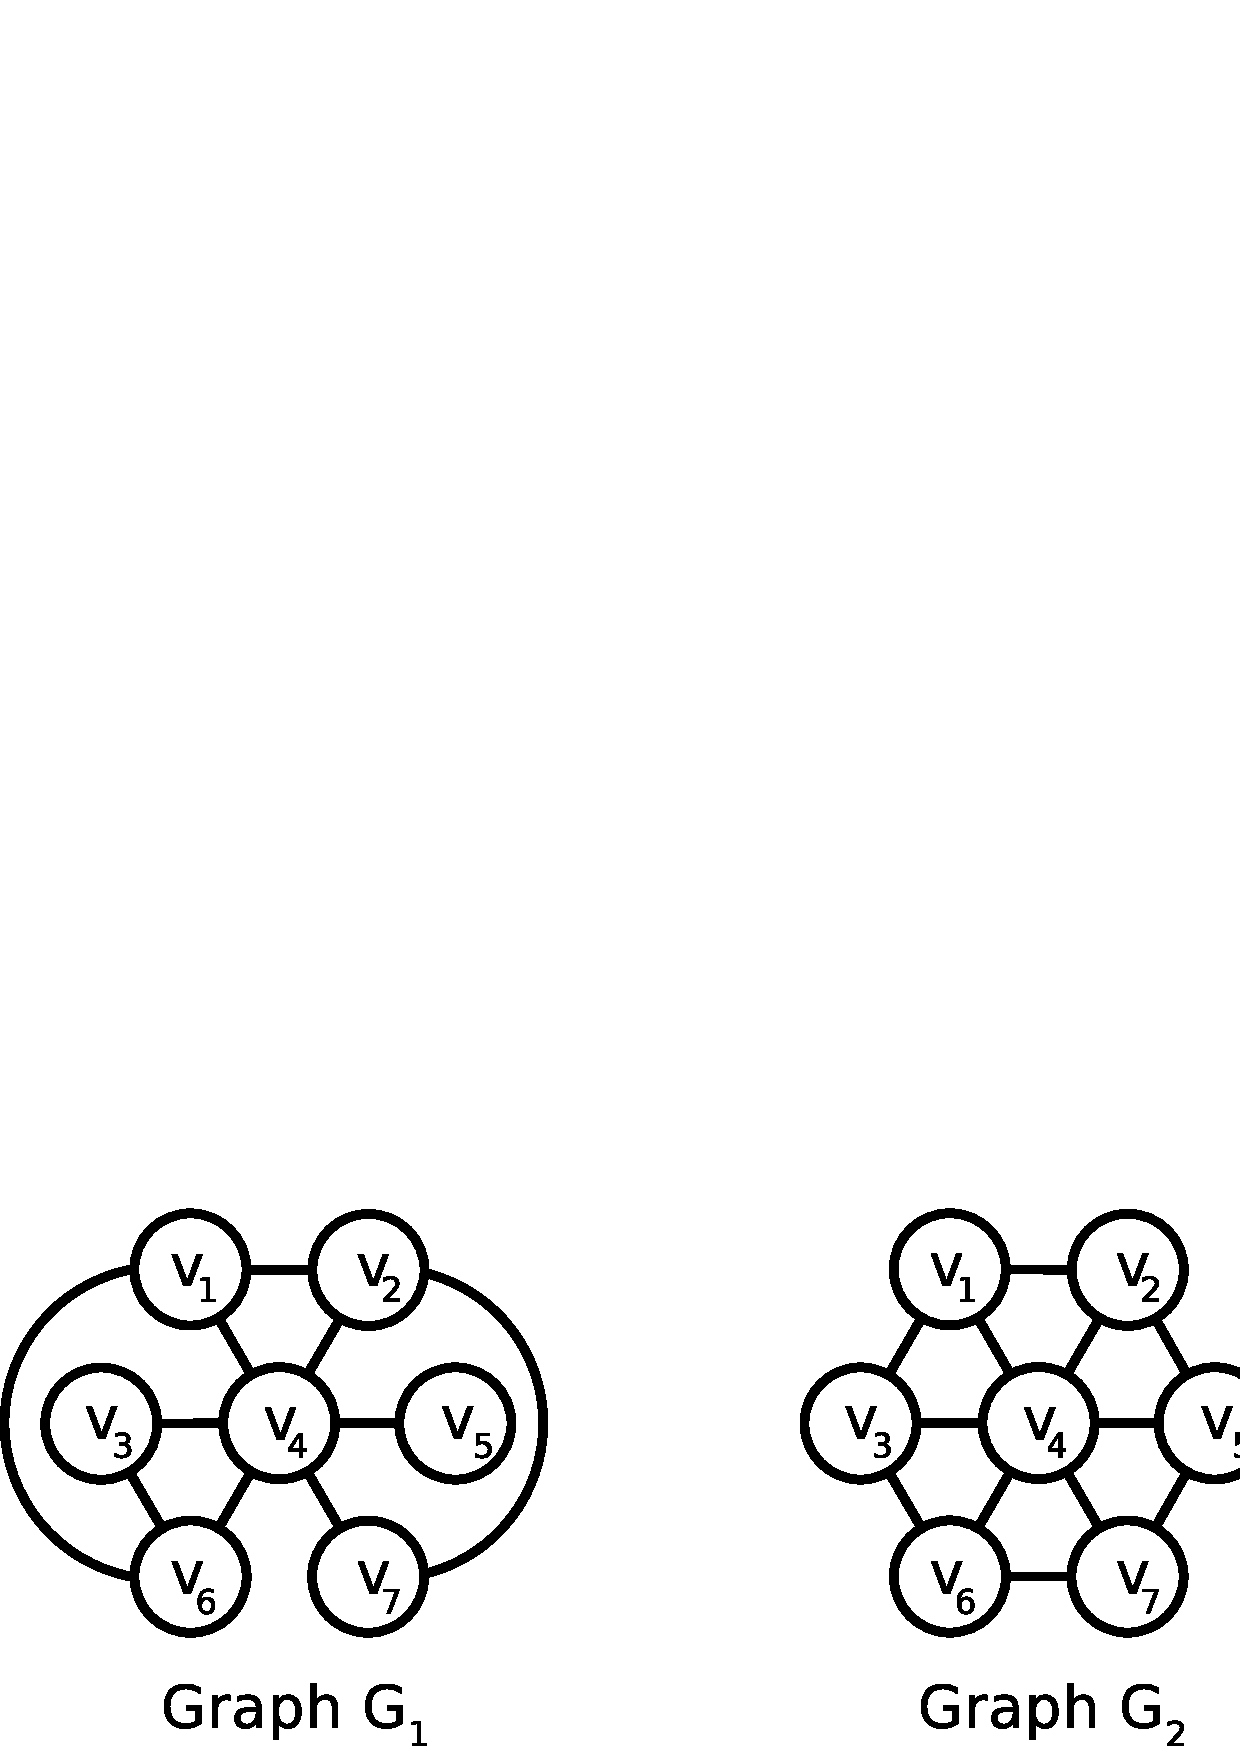
\includegraphics[width=430pt]{bilder/bsp2.pdf}
	\caption{Vier Beispielgraphen}
  	 \end{figure}
  	 ~\newline  	 
Der Graph $G_3$ ist ein Teilgraph der Graphen $G_1$ und $G_2$. Der Graph $G_4$ ist ein induzierter Teilgraph von dem Graphen $G_1$, welcher durch das Löschen des Knotens $v_4$ entsteht. Durch das Löschen von den Kanten $\{v_1,v_3\}$,$\{v_2,v_5\}$,$\{v_5,v_7\}$ und $\{v_6,v_7\}$ in Graphen $G_2$ entsteht ein Teilgraph des Graphen $G_1$.
\end{bsp}
\subsection{Kürzeste Wege}
Ein \emph{Weg} $p$ in $G$ von Knoten $u$ nach Knoten $w$ ist eine Folge von Knoten $$p=(v_1,\ldots,v_j)$$ mit $v_1=u$ und $v_j=w$ mit $\{v_{i-1},v_i\}\in E$ für $1 <i \leq j$.\\Der Knoten $u$ wird als \emph{Startknoten} bezeichnet und der Knoten $w$ als \emph{Endknoten}.% Bei einem \emph{Kreis} ist der Startknoten gleich mit dem Endknoten $u=v$.
\\Einen Weg $p$ nennt man \emph{einfach}, wenn alle Knoten $v_1,\ldots,v_j$ paarweise verschieden sind. Zwei Wege sind \emph{knotendisjunkt} sofern alle Knoten auf diesem Weg, ausgenommen Start- und Endknoten, paarweise verschieden sind. Die \emph{Länge} eines Weges $p$ von Knoten $u$ nach Knoten $w$ entspricht der Anzahl seiner Kanten.\\
Die \emph{Distanz} $dist_G(u,w)$ zweier Knoten $u,w$ eines Graphen $G$ ist die \emph{Länge des kürzesten Weges} in $G$ zwischen $u$ und $w$, falls mindestens ein solcher Weg existiert, ansonsten ist die kürzeste Weglänge $\infty$. Der \emph{Durchmesser} $diam(G)$ eines Graphen ist die maximale Distanz aller Knotenpaare aus $G$.
\todo[inline]{Kreis,einfacher Kreis, Überarbeiten Länge etc.}
\begin{bsp}
Sei der Graph $G=(V,E)$ gegeben. Eine möglichen Einbettung in der Ebene könnte wie folgt aussehen:\\
\begin{figure}[h!]
		\centering 		 
   \includegraphics[width=260pt]{bilder/bsp3.pdf}
	\caption{Graph $G$}
  	 \end{figure}
  	 \\
Zwischen Knoten $v_1$ und $v_2$ gibt es mehrere einfache Wege mit unterschiedlicher Länge. Der kürzeste Weg geht über vier Kanten und damit ist $dist_G(v_1, v_2)=4$. Der Durchmesser $diam(G)=5$, denn $dist_G(v_3, v_4)=5$.
\end{bsp}
\subsection{Zusammenhangskomponenten}
Zwei Knoten $a$ und $b$ eines Graphen $G$ heißen \emph{verbunden} in $G$, wenn $a = b$ ist oder es einen Weg in $G$ von $a$ nach $b$ gibt.\\Ist jedes Knotenpaar in $G$ verbunden, so heißt $G$ \emph{zusammenhängend}.\\Gibt es zwischen jedem Knotenpaar zwei (bzw. $k$) knotendisjunkte Wege, so bezeichnet man den Graphen als \emph{zweifach ($k$-fach) zusammenhängend}.\\Eine $k$-fache Zusammenhangskomponente von $G$ ist ein maximaler (bzgl. der Knotenmenge) $k$-fach zusammenhängender, induzierter Teilgraph von $G$.
\subsection{Trennungsknoten und Bifurkatoren}
\begin{figure}[ht]
\centering
\includegraphics*[width = 200pt]{bilder/bifurkator.pdf}
\caption{Beispiel für einen Bifurkator}
\label{bild:bifurkator}
\end{figure}  	 
Sei ein Graph $G=(V,E)$ gegeben. Für die Knoten $z,x$ und $y$ besteht die Menge $B$ aus allen Knoten, die gleichzeitig auf einem kürzesten Weg von $z$ zu $x$ und auf einem kürzesten Weg von $z$ zu $y$ liegen. Ein Knoten $v$ aus der Menge $B$ mit maximaler Distanz zum Knoten $z$ wird als ein \emph{Bifurkator} von $z, x, y$ bezeichnet.\newline
Sind zwei Knoten $u,v$ durch die Entfernung eines Trennungsknotens $x$ in zwei unterschiedlichen Teilgraphen, so liegt der Knoten $x$ auf jedem Wege von $u$ nach $v$.
\todo[inline]{def: Trennungsknoten, Kontraktion, Erweiterung, NP und Laufzeit}
%%%%%%%%%%%%%%%%%%%%%%%%%%%%%%%%%%%%%%%%%%%%%%%%%%%%%%%%%%%%%%%%%%%%%%%%%%%%%%%%%%%%%%%%%%%%%%%%%%%%%%%%%%%%%%%%
\newpage
\section{Metrische Dimension}
\label{MDT}
\begin{defi}{\textbf{(Metrische Dimension)}}\\
Ein Knoten $x$ eines Graphens $G$ \emph{trennt} zwei Knoten $u$ und $v$ in $G$ sofern $d(x, u) \neq d(x, v)$. Eine Knotenmenge $R'$ von $G$ ist eine \emph{trennende Menge} von $G$ sofern alle Knoten in $G$ durch mindestens einen Knoten in $R$ getrennt werden. Eine \emph{metrische Basis} $R$ von $G$ ist eine trennende Menge mit minimaler Anzahl von Elementen, und jeder Knoten aus der metrischen Basis ist ein \emph{Ankerknoten}. % welche nicht eindeutig sein muss\todo{Gibt es eindeutige MB für $|V|>1$}.
Die metrische Dimension $\beta(G)$ von $G$ ist die Kardinalität einer metrischen Basis. Für eine metrische Basis mit einer Anordnung $$R_n = \{r_1 , \ldots , r_n \} \subseteq V (G)$$ und einen Knoten $v \in V (G)$ wird $(d(v, r_1 ), \ldots , d(v, r_n ))$ als der Vektor der \emph{metrischen Koordinaten} von $v$ bezeichnet.
\end{defi}
\begin{bsp}
\end{bsp}
\begin{bem}
In Zeichnungen werden Knoten aus der metrischen Basis grau gekenntzeichnet und der Vektor der metrischen Koordinaten wird in roter Farbe neben dem Knoten $v$ in der Form $d(v, r_1 )/ \ldots / d(v, r_n )$ beschriftet. In Beschreibungen wird dieser auch Markierung eines Knotens genannt. Sofern zwei oder mehr Knoten durch eine bereits markierte Knotenmenge nicht getrennt werden, werden diese rot gekennzeichnet. 
\end{bem}
%%%%%%%%%%%%%%%%%%%%%%%%%%%%%%%%%%%%%%%%%%%%%%%%%%%%%%%%%%%%%%%%%%%%%%%%%%%%%%%%%%%%%%%%%%%%%%%%%%%%%%%%%%%%%%%%
\section{Bekannte Resultate zur metrischen Dimension}
Die metrischen Dimension ist bei einigen Graphklassen konstant. Ein Beispiel dafür sind Kreise $C_n$ mit $n\geq 3$ und $md(C_n)=2$. Weiterhin existieren Graphklassen mit größen bzw. parameterabhängiger metrischer Dimension wie z.B. die vollständigen Graphen $K_n$ mit $n \geq 1$ und $md(K_n)=n-1$.\newline Bei manchen Klassen kann die metrische Dimension nur algorithmisch bestimmt werden, wie z.B. bei Bäumen oder bei außenplanaren Graphen.\cite{}\newline
Neben diesen Erfolgen gibt es außerdem Resultate über die NP-Vollständigkeit der Berechnung. So ist die Bestimmung der metrischen Dimension für allgemeine Graphen \cite{} und für planare \cite{}, bipartite \cite{} und Unit-Disk Graphen \cite{} ein NP-Vollständiges Problem.\newline\newline
{\textbf{Graphen mit fester und parameterabhängiger metrischer Dimension}}
\begin{lem}
\label{path}\cite{landmarks}
Die metrische Dimension eines Graphen $G$ ist genau dann eins wenn der Graph $G$ der Weg $P_n$ ist.
\end{lem}
\begin{lem}
\label{complete}\cite{landmarks}
Die metrische Dimension eines Graphen $G$ ist genau dann $n-1$ wenn der Graph $G$ der vollständige Graph $K_n$ ist.
\end{lem}
\begin{lem}\cite{landmarks}
Sei $G = (V, E)$ ein Graph mit $n$ Knoten und metrischer Dimension $n-2$, dann gilt eine der folgenden Aussagen:
\begin{enumerate}
\item Der $K_{r,s}$ mit $r,s \geq 1$.
\item Der $K_{r}+ \overline{K_s}$ mit $r,s \geq 1$.
\item oder der $K_{r,s}$ mit $r,s \geq 1$.
\end{enumerate}
\todo[inline]{n-3}
\end{lem}
Eine Übersicht über die metrische Dimension einiger Graphklassen:
  \begin{table}[htb]
     \centering
     \begin{tabularx}{\textwidth}{|c|c|c|c|c|c|}
     	\hline  
       \parbox[c][5em][c]{0pt}{~}\textbf{Graphklasse} $G$ & $C_n$&$K_{n,m}$&$S_{1,n}$&$W_{1,n}$, $n \in \{3,6\}$&$W_{1,n}$ sonst \\[2em]
		\hline       
       \parbox[c][5em][c]{0pt}{~}\textbf{Metr. Dimension $\beta(G)$}& $2$&$min(n,m)+1$& $n-1$  &$3$  &$\lfloor \dfrac{2n+2}{5} \rfloor$        \\[2em]
       	\hline  
     \end{tabularx}
 
     \caption{Metrische Dimension einiger Graphklassen}
     \label{tbl:Metrische Dimension einiger Graphklassen}
     % Verweis im Text mittels \ref{tbl:Metrische Dimension einiger Graphklassen}
   \end{table}
~\newline
Manche Ergebnisse wurden zwischenzeitlich für falsch erklärt. 
\begin{lem}(\cite{landmarks} und als falsch erklärt in \cite{somefamiliesofgraphs})
Es gilt $\beta(P_m \square P_n)=2$ (2-dimensionales Gitter $n \times m$) aber ein $d-$dimensionales Gitter $G_d$ hat $\beta(G_d) \neq d$ für $d \geq 3$.
\end{lem}
Bei einem gegebenen Graphen und seiner metrischen Dimension kann man einige Teilgraphen im voraus ausschließen und auch Aussagen über den Graphen treffen.
\begin{lem}
Ein Graph $G$ mit $\beta(G) = k$ kann keinen $K_{2k+1}$ als Teilgraph beinhalten.\cite{landmarks}
\end{lem}
\begin{lem}\cite{landmarks}
Sei $G = (V, E)$ ein Graph mit metrischer Dimension zwei, dann gilt, dass der $K_{5}$, so wie der $K_{3,3}$ keine Teilgraphen von $G$ sind.
\end{lem}
\begin{lem}\cite{landmarks}
Sei $G = (V, E)$ ein Graph mit metrischer Dimension zwei und sei $\{a, b\} \subset V$ eine metrische Basis von $G$. Dann gilt folgendes:
\begin{enumerate}
\item Es existiert ein eindeutiger kürzester Weg $P$ zwischen $a$ und $b$.
\item Der Grad von $a$ und $b$ ist höchstens drei.
\item Jeder anderen Knoten auf dem Weg $P$ hat höchstens den Grad fünf.
\end{enumerate}
\end{lem}
\textbf{Algorithmen zur metrischen Dimension}
\begin{lem}\cite{landmarks} 
Die metrische Dimension eines Baumes $T$, welcher kein Weg ist, lässt sich berechnen durch $\Sigma_{v \in V:L_v >1} (l_v-1)$. Dabei ist $l_v$ die Anzahl der Brücken welche Wege sind am Knoten $v$.
\end{lem}
\begin{lem}\cite{onthecomplexity}
Sei ein außenplanarer Graph $G=(V,E)$ gegeben. Dann kann $\beta(G)$ in Polynomialzeit berechnet werden.
\end{lem}
\textbf{NP-Vollständigkeits- Resultate}
\begin{defi}[Entscheidungs- und Minimierungsproblem]~\newline
\vspace{-7mm}
\EP{{Metrische Dimension Enscheidungsproblem}}
{Ein ungerichteter Graph $G=(V,E)$ und eine natürlich Zahl $k$.}
{Gibt es eine metrische Basis der Größe höchstens $k$?}
\vspace{-2mm}
\centering und
\vspace{-1mm}
\MP{{Metrische Dimension Minimierungsproblem}}
{Ein ungerichteter Graph $G=(V,E)$.}
{Die metrische Dimension $k$ oder\\&die Größe $k$ einer kleinsten trennenden Menge (metrischen Basis).}
\end{defi}
\begin{lem}\cite{onthecomplexity}
Sei ein Graph $G=(V,E)$ gegeben. Das Minimierungsproblem für das Finden der metrischen Dimension von $G$ ist NP-vollständig.
\end{lem}
\begin{lem}\cite{onthecomplexity}
Sei ein planarer Graph $G=(V,E)$ gegeben. Das Minimierungsproblem für das Finden der metrischen Dimension von $G$ ist NP-vollständig.
\end{lem}
\begin{lem}\cite{anefficientrepresentationofbenesnetworksanditsapplications}
Sei ein bipartiter Graph $G=(V,E)$ gegeben. Das Minimierungsproblem für das Finden der metrischen Dimension von $G$ ist NP-vollständig.
\end{lem}
\textbf{Approximierbarkeit der metrischen Dimension}
\begin{lem}\cite{landmarks}
Sei ein Graph $G=(V,E)$ mit $n$ Knoten gegeben. Dann kann $\beta(G)$ in Polynomialzeit approximiert werden mit einem Faktor $f$ mit $f \in \mathcal{O}(log\:n)$.
\end{lem}
\newpage
\section{Weitere Dimensionen von Graphen}
Neben der metrischen Dimension gibt es andere ähnliche auf Graphen definierte Probleme, die leicht in Zusammenhang mit dieser gebracht werden können oder sich sogar aus der metrischen Dimension herleiten.
\subsection{Partitionsdimension}
Im Jahre 1998 entwickelten Chartrand, Zhang and Salehi in ihrer Arbeit "On the partition dimension of a graph" [CZS98] aus der metrischen Dimension die Partitionsdimension $pd(G)$. Während bei der metrischen Dimension nur einzelne Knoten in die Basis aufgenommen werden, dürfen bei der Partitionsdimension Mengen von Knoten aufgenommen werden. Weiterhin muss die gesuchte Partition $\Pi = \{S_1, S_2, \ldots, S_k\}$ jeden Knoten trennen und den gesamten Graphen in Mengen aufteilen. Dabei wird versucht die Anzahl der Mengen minimal zu halten. Die Partitionsdimension des Graphen $pd(G)$ ist die kleinste Anzahl von Mengen.\\
Für die Distanz eines Knoten gilt dabei $d(v,S_i)=min\{d(v,x) \mid x\in S_i\}$.\newline
Beispiel\newline
Resultate und Zusammenhang mit der metrischen Dimension\newline
\subsection{Oberdimension}


%%%%%%%%%%%%%%%%%%%%%%%%%%%%%%%%%%%%%%%%%%%%%%%%%%%%%%%%%%%%%%%%%%%%%%%%%%%%%%%%%%%%%%%%%%%%%%%%%%%%%%%%%%%%%%%%
%%%%%%%%%%%%%%%%%%%%%%%%%%%%%%%%%%%%%%%%%%%%%%%%%%%%%%%%%%%%%%%%%%%%%%%%%%%%%%%%%%%%%%%%%%%%%%%%%%%%%%%%%%%%%%%%
%%%%%%%%%%%%%%%%%%%%%%%%%%%%%%%%%%%%%%%%%%%%%%%%%%%%%%%%%%%%%%%%%%%%%%%%%%%%%%%%%%%%%%%%%%%%%%%%%%%%%%%%%%%%%%%%
\chapter{Eigenschaften der metrische Dimension}
\section{Metrische Dimension von zusammengestellten Graphen}
\label{kapallg}
Es seien mehrere Graphen mit bekannter metrische Dimension gegeben.\newline Welche Aussagen bezüglich metrischer Dimension lassen sich über unterschiedliche Kompositionen oder Teilgraphen von diesen Graphen formen?\\Dieser Abschnitt widmet sich einerseits der bekannten und bereits erforschten Vereinigung und kartesische Produkt von zwei Graphen. Weiterhin werden die $r-$fachen Verschmelzung und $r-$fachen Vereinigung von zwei Graphen definiert und Aussagen über ihre metrische Dimension gemacht.\\Bei der Vereinigung und dem kartesischen Produkt werden alle Knoten an der Komposition beteiligt, bei dem Corona Produkt wird ein Graph kopiert und mit jedem Knoten von dem anderen Graphen verbunden und bei der $r-$fachen Verschmelzung werden die Knoten mit einer Ordnung versehen und zwei gleichmächtige Folgen von Knoten mit übergeben.   
\begin{defi}{\textbf{(Vereinigung)}}\\
Gegeben seien zwei Graphen $G_1=(V_1,E_1)$ und $G_2=(V_2,E_2)$. Durch die Vereinigung $G_{1+2}=G_1+G_2$ entsteht der Graph mit der Knotenmenge $V_{1+2}=V_1 \cup V_2$ und der Kantenmenge $E_{1+2}= E_1 \cup E_2 \cup \{\{v_1,v_2\}| v_1 \in V_1 \wedge v_2 \in V_2\}$.
\end{defi}

\begin{defi}{\textbf{(Kartesisches Produkt)}}\\
Gegeben seien zwei Graphen $G_1=(V_1,E_1)$ und $G_2=(V_2,E_2)$. Durch das kartesische Produkt $G_{1\square 2}=G_1 \square G_2$ entsteht der Graph mit der Knotenmenge $V_{1 \square 2}=V_1 \times V_2$ und der Kantenmenge $E_{1\square 2}= \{\{(x_1,x_2),(y_1,y_2)\}| (x_1=y_1 \wedge \{x_2,y_2\} \in E_2)\vee (x_2=y_2 \wedge \{x_1,y_1\} \in E_1)\}$. 
\end{defi}

\begin{defi}{\textbf{(Corona Produkt)}}\\
Gegeben seien zwei Graphen $G_1=(V_1,E_1)$ und $G_2=(V_2,E_2)$. Durch das Corona Produkt $G_1 \odot G_2$ wird der Graph $G_2$ $|V_1|$-mal kopiert und jeder Knoten von dem $i$-ten $G_2$ wird mit dem $i$-ten Knoten in $V_1$ verbunden.
\end{defi}

\begin{defi}{\textbf{($r-$fache Verschmelzung)}}\\
Gegeben seien zwei Graphen $G_1=(V_1,E_1)$ und $G_2=(V_2,E_2)$ mit $|V_1|, |V_2| \geq r$ und zwei Teilfolgen $V'_{1} \subseteq V_1$ und $V'_{2} \subseteq V_2$ mit $|V'_{1}|, |V'_{2}| = r$. Aus der $r-$fachen Verschmelzung $G_{1 \infty 2}=G_1 \infty G_2$ entsteht der Graph mit der Knotenmenge $V_{1 \infty 2}=V_1 \cup V_2\backslash V'_{2}$ und der Kantenmenge $E_{1\infty 2}= E_1 \cup E_2$. Außerdem gilt, dass der $i-$te Knoten aus $V'_{1}$ mit dem $i-$ten Knoten aus $V_{2,r}$ für $1 \leq i \leq r$ verschmolzen wird. 
\end{defi}

\begin{bsp} ~ \newline
Gegeben seien $G_1=P_4$ mit $deg(v_1)=deg(v_2)=1$ und $G_2=C_3$.\\Die Knoten aus den Mengen $V'_1$ und $V'_2$ sind in der Abbildung \ref{bild:vereinigung} farblich markiert und mit ihrer Bezeichnung versehen.
\begin{figure}[h!]
		\centering 		 
   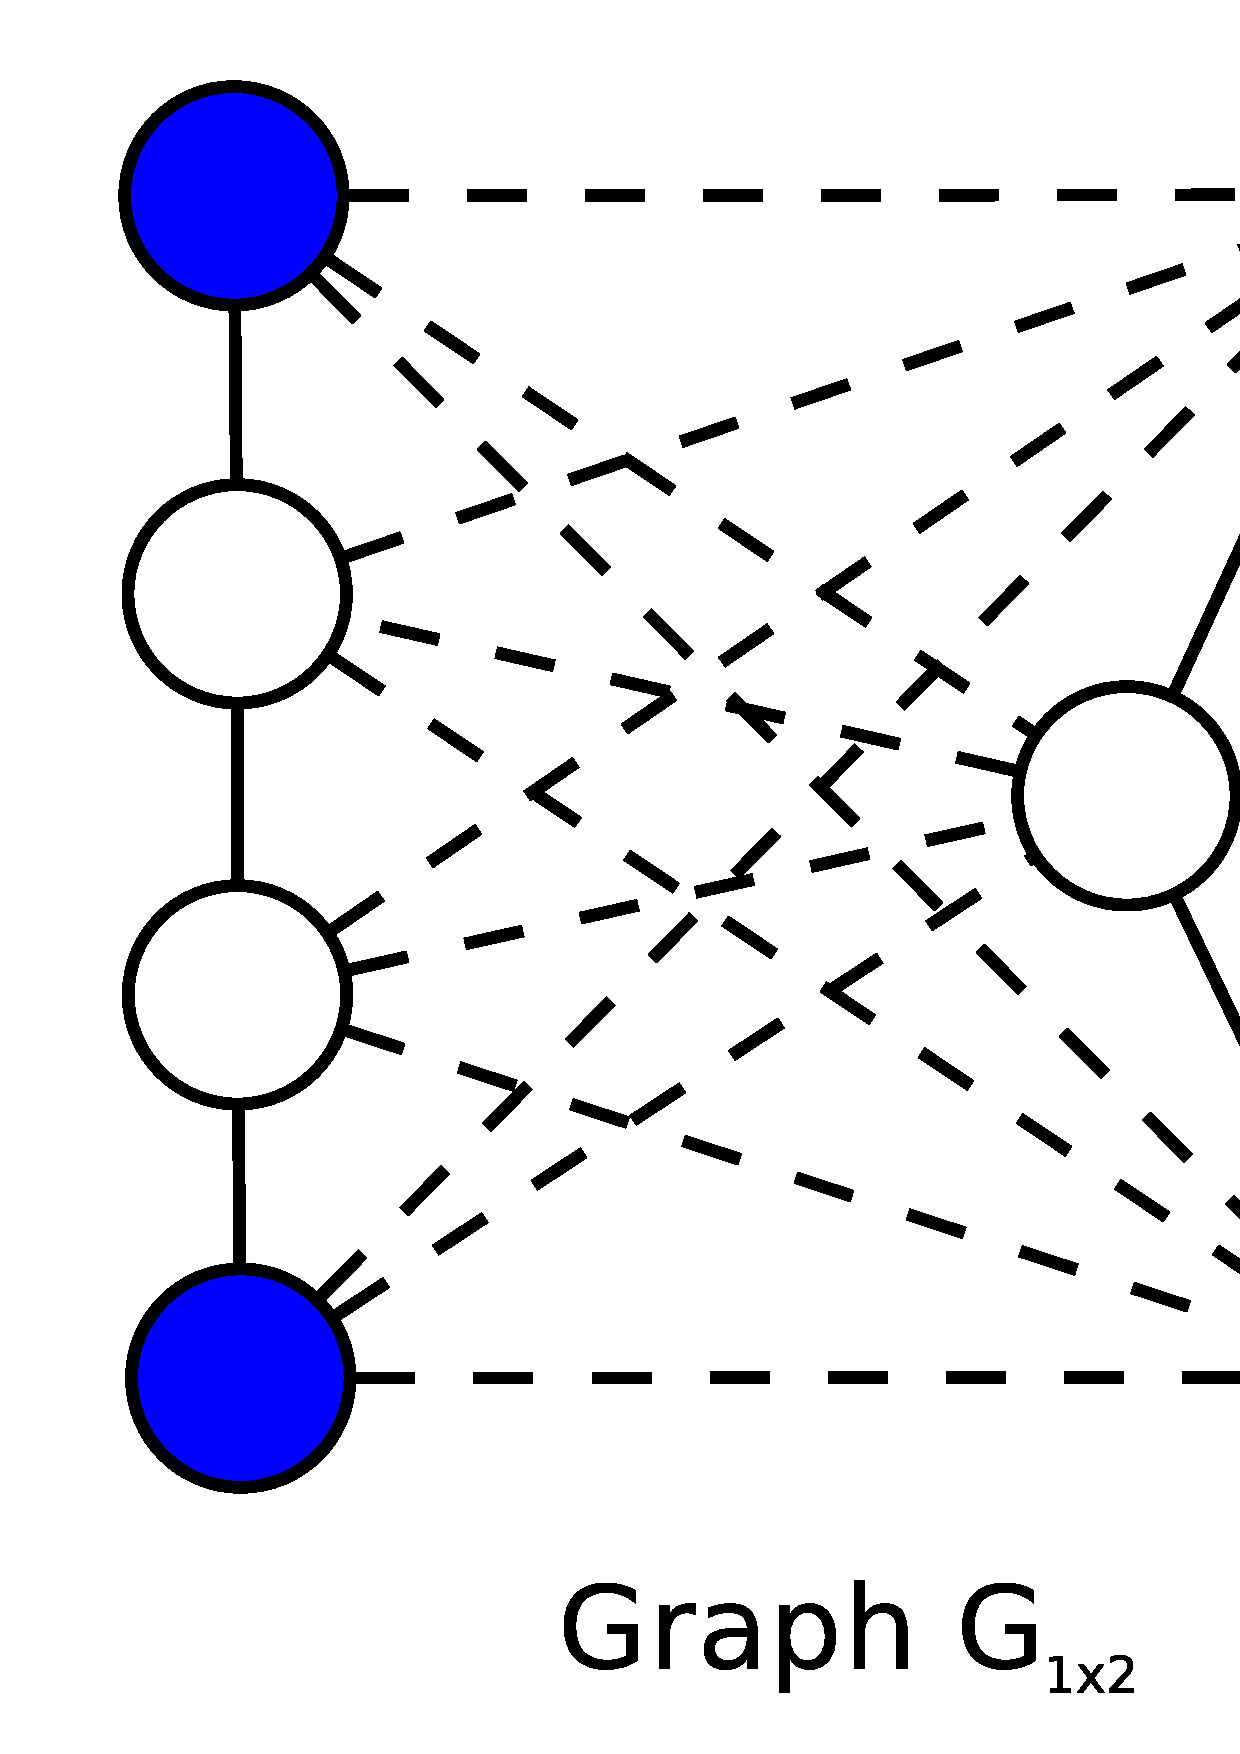
\includegraphics[width=350pt]{bilder/struktur2.pdf}
	\caption{Beispiel für Vereinigung, kartesisches Produkt, Corona Produkt und $r-$fache Verschmelzung}
  	 \label{bild:vereinigung}
  	 \end{figure}
\end{bsp}
\begin{lem}(Ergebnisse zur Vereinigung, zum kartesischen und Corona Produkt \cite{somefamiliesofgraphs})\newline
Sei $G=(V,E)$ ein beliebiger Graph.
\begin{itemize}
\item $max\{\beta(G),\beta(H)\}\leq \beta(G\square H) \leq min\{\beta(G)+|H|,\beta(H)+|G|\}-1$
\item $2 \leq \beta(G) \leq \beta(H) \leq \beta(G\square H) \leq min\{\beta(G)+|H|,\beta(H)+|G|\}-2$
\item $\beta(G)+\beta(H) \leq \beta(G+H)$
\item $\beta(G)\leq \beta(G\square K_2) \leq \beta(G)+1$
\item $\beta(G)\leq \beta(G\square P_n) \leq \beta(G)+1$
\item $\beta(G\square K_n) \leq \beta(G)+n-2$ für $n \geq 3$
\item $\beta(G\square C_n) \leq \beta(G)+1$ für $n$ ungerade und $\beta(G\square C_n) \leq \beta(G)+2$ für $n$ gerade
\item $\beta(P_m+P_n)=2$
\item $\beta(P_m+K_n)=n-1$ für $n\geq 3$
\item $\beta(P_m+C_n)=2$ für $n$ ungerade
\item $\beta(P_m+C_n)=2$ für $n$ gerade und $m \neq 1$
\item $\beta(C_m+C_n)=3$ falls $m$ oder $n$ gerade
\item $\beta(C_m+C_n)=4$ sonst
\item $\beta(K_m+C_n)=m$ falls $m=4$ und $n$ ungerade
\item $\beta(K_m+C_n)=m-1$ sonst
\end{itemize}
\end{lem}
\begin{comment}
Ergebnisse für die Vereinigung von festen Graphklassen\cite{somefamiliesofgraphs}:
 \begin{table}[htb]
     \centering
     \begin{tabularx}{\textwidth}{|c|c|c|c|c|c|}
     	\hline
     	& $P_n$&\multicolumn{2}{c|}{$C_n$}&\multicolumn{2}{c|}{$K_n$}\\
		\hline
		$P_m$&$2$&\multicolumn{2}{c|}{$2$}&\multicolumn{2}{c|}{$n-1$}\\
       	\hline
       	\multirow{2}{*}{$C_m$}&\multirow{2}{*}{$2$}&$3$&$m$ oder $n$ gerade& $m$  &$m=4$ und $n$ ungerade\\
       	\cline{3-6}
       	     &	 &$4$&sonst		   	  & $m-1$&sonst\\
       	\hline
       	\multirow{2}{*}{$K_m$}&\multirow{2}{*}{$m-1$}&$m$&$m=4$ und $n$ ungerade &\multicolumn{2}{c|}{$m+n-1$}\\
       		\cline{3-4}
       	&&$m-1$&sonst&\multicolumn{2}{c|}{}\\
       	\hline
       	\end{tabularx}
 
     \caption{Metrische Dimension der Vereinigung einiger Graphklassen}
     \label{tbl:Metrische Dimension der Vereinigung einiger Graphklassen}
     % Verweis im Text mittels \ref{tbl:Metrische Dimension einiger Graphklassen}
   \end{table}
\end{comment}   
\begin{lem}$\;\;$\\Folgende Schranken gelten für die $r-$fache Verschmelzung von Graphen mit $r \geq 4$:
$$\beta(G_1)+\beta(G_2)-2r \leq \beta(G_1 \infty G_2) \leq \beta(G_1)+\beta(G_2)+r+2 \cdot \lfloor\frac{(r-2)}{3}\rfloor+1$$
\end{lem}

\begin{proof}[Beweis:] 
Um zu zeigen, dass die Schranken strikt, sind werden zwei folgende Klassen von Graphen betrachtet. Für die obere Schranke gilt:\\
\begin{figure}[ht]
		\centering 		 
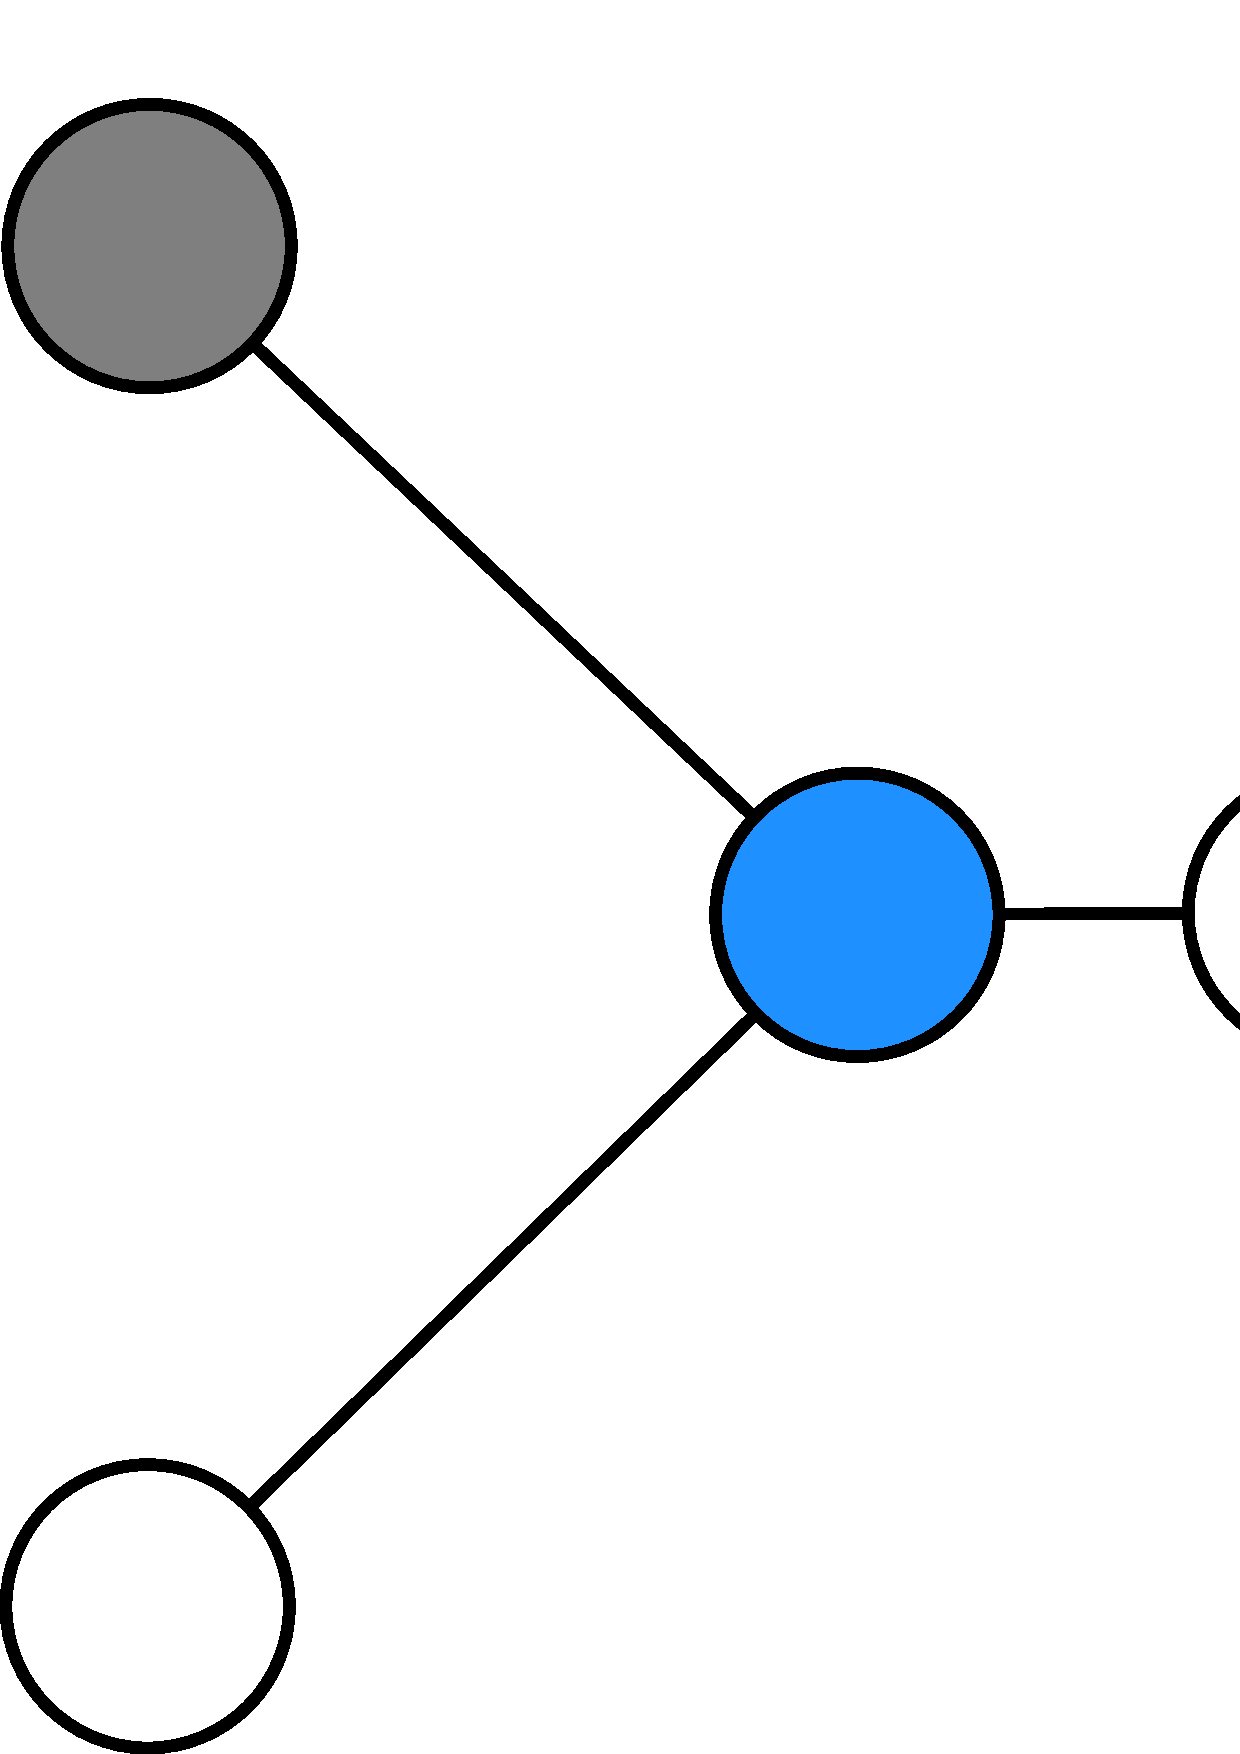
\includegraphics[width=420pt]{bilder/ver.pdf}
   \caption{Graph $G_1$ mit der metrischen Dimension $2$}
   \label{bild:Graphmd2}
  	 \end{figure}
\\
Betrachte man den Graphen $G_1$ aus der Abbildung \ref{bild:Graphmd2}.
Um zu zeigen das $\beta(G_1)=2$ betrachte die einzelnen Komponenten des Graphen. Nach Lemma \ref{path} ist bekannt, dass die metrische Dimension eines Weges eins ist. Aufgrund der zwei Blätter am linken und rechten Rand, werden mindestens zwei Knoten in der metrischen Basis benötigt, einer aus den linken und einer aus den beiden rechten Blättern. Die Knoten aus der trennenden Menge wurden in der Abbildung \ref{bild:Graphmd2} markiert.\\ Um zu sehen, dass diese zwei Knoten den Graphen trennen, betrachte, dazu die provisorischen Markierungen in der Abbildung \ref{bild:Kreise}.
\begin{figure}[h!]
		\centering 		 
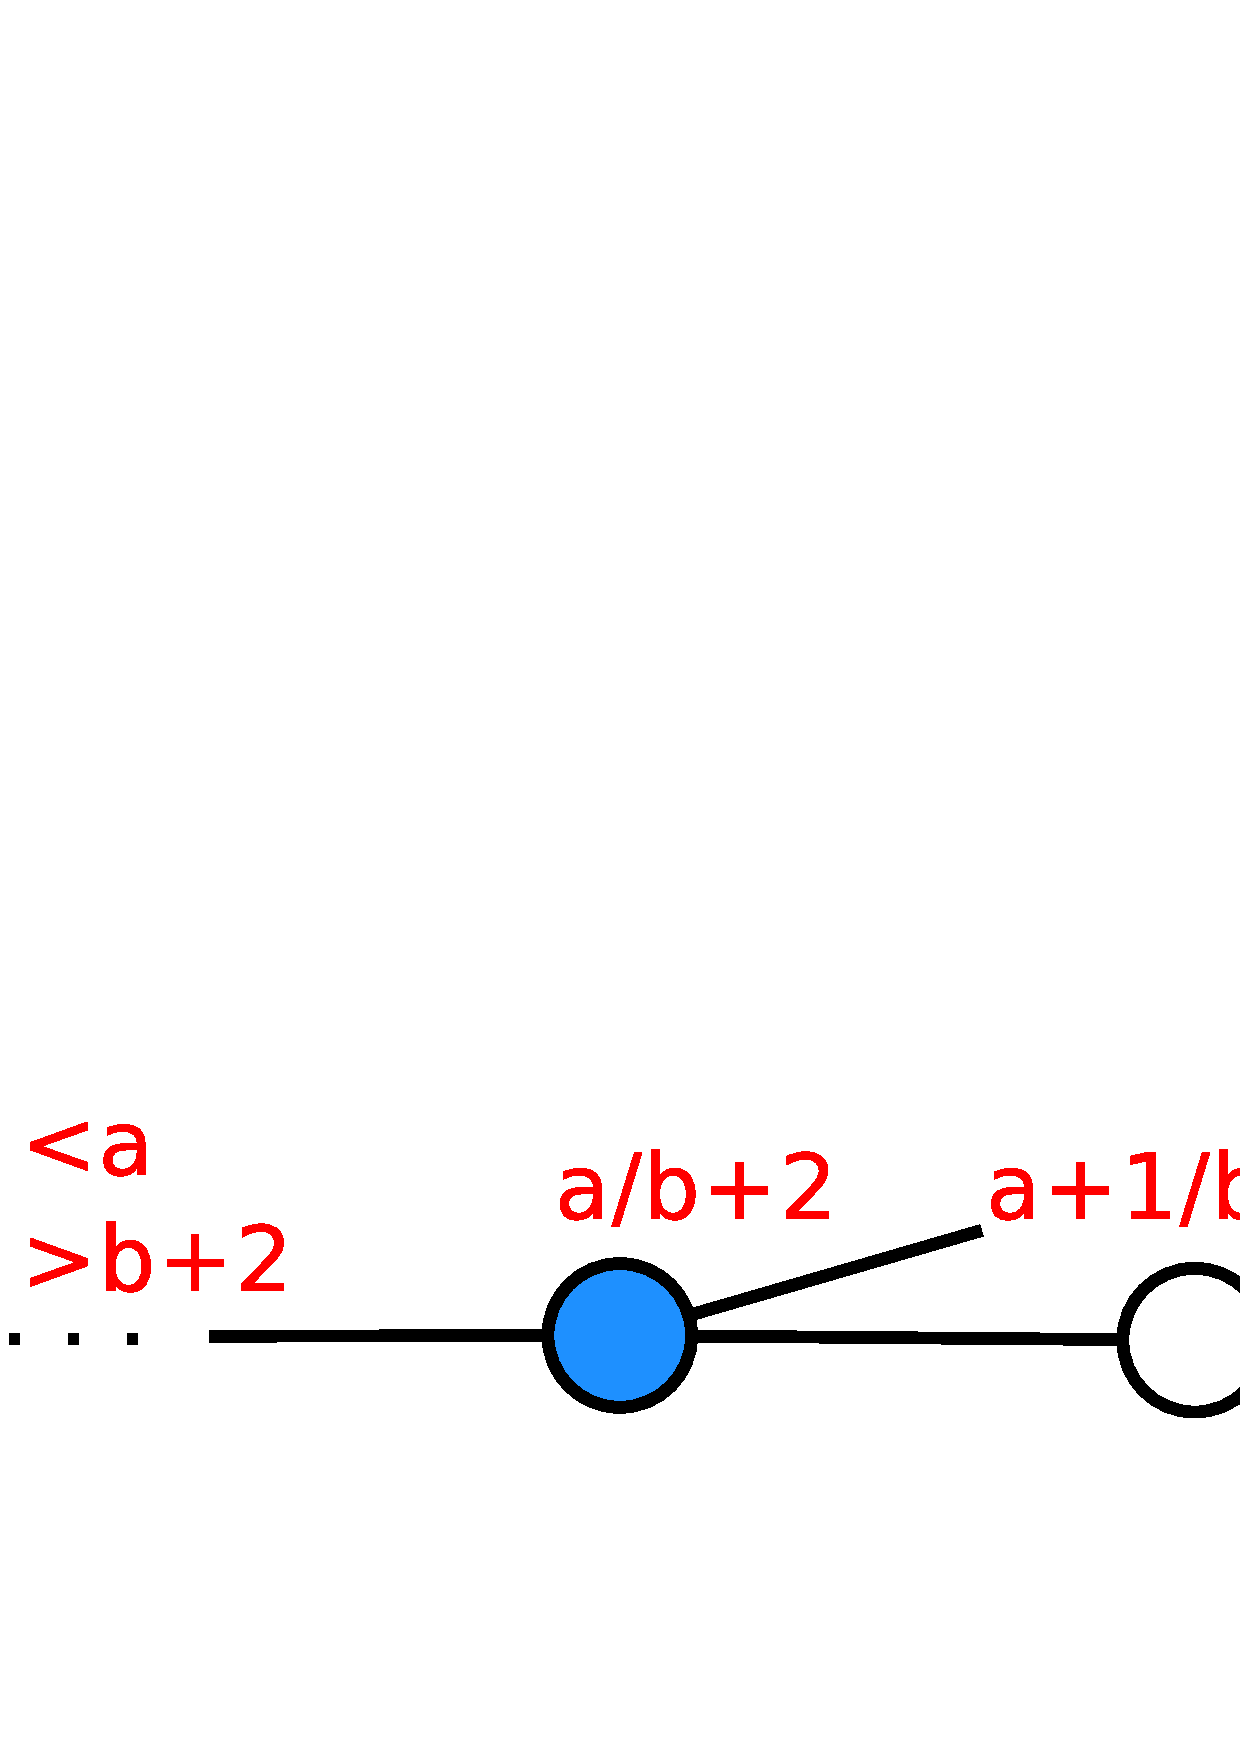
\includegraphics[width=420pt]{bilder/ver2.pdf}
   \caption{Kreise der Länge 6 in Graphen $G_1$}
   \label{bild:Kreise}
  	 \end{figure} 
  	 
Erzeuge einen äquivalenten Graphen $G_2$ mit welchem $G_1$ verschmolzen wird, so entsteht der folgenden Graph:

\begin{figure}[h!]
		\centering 		 
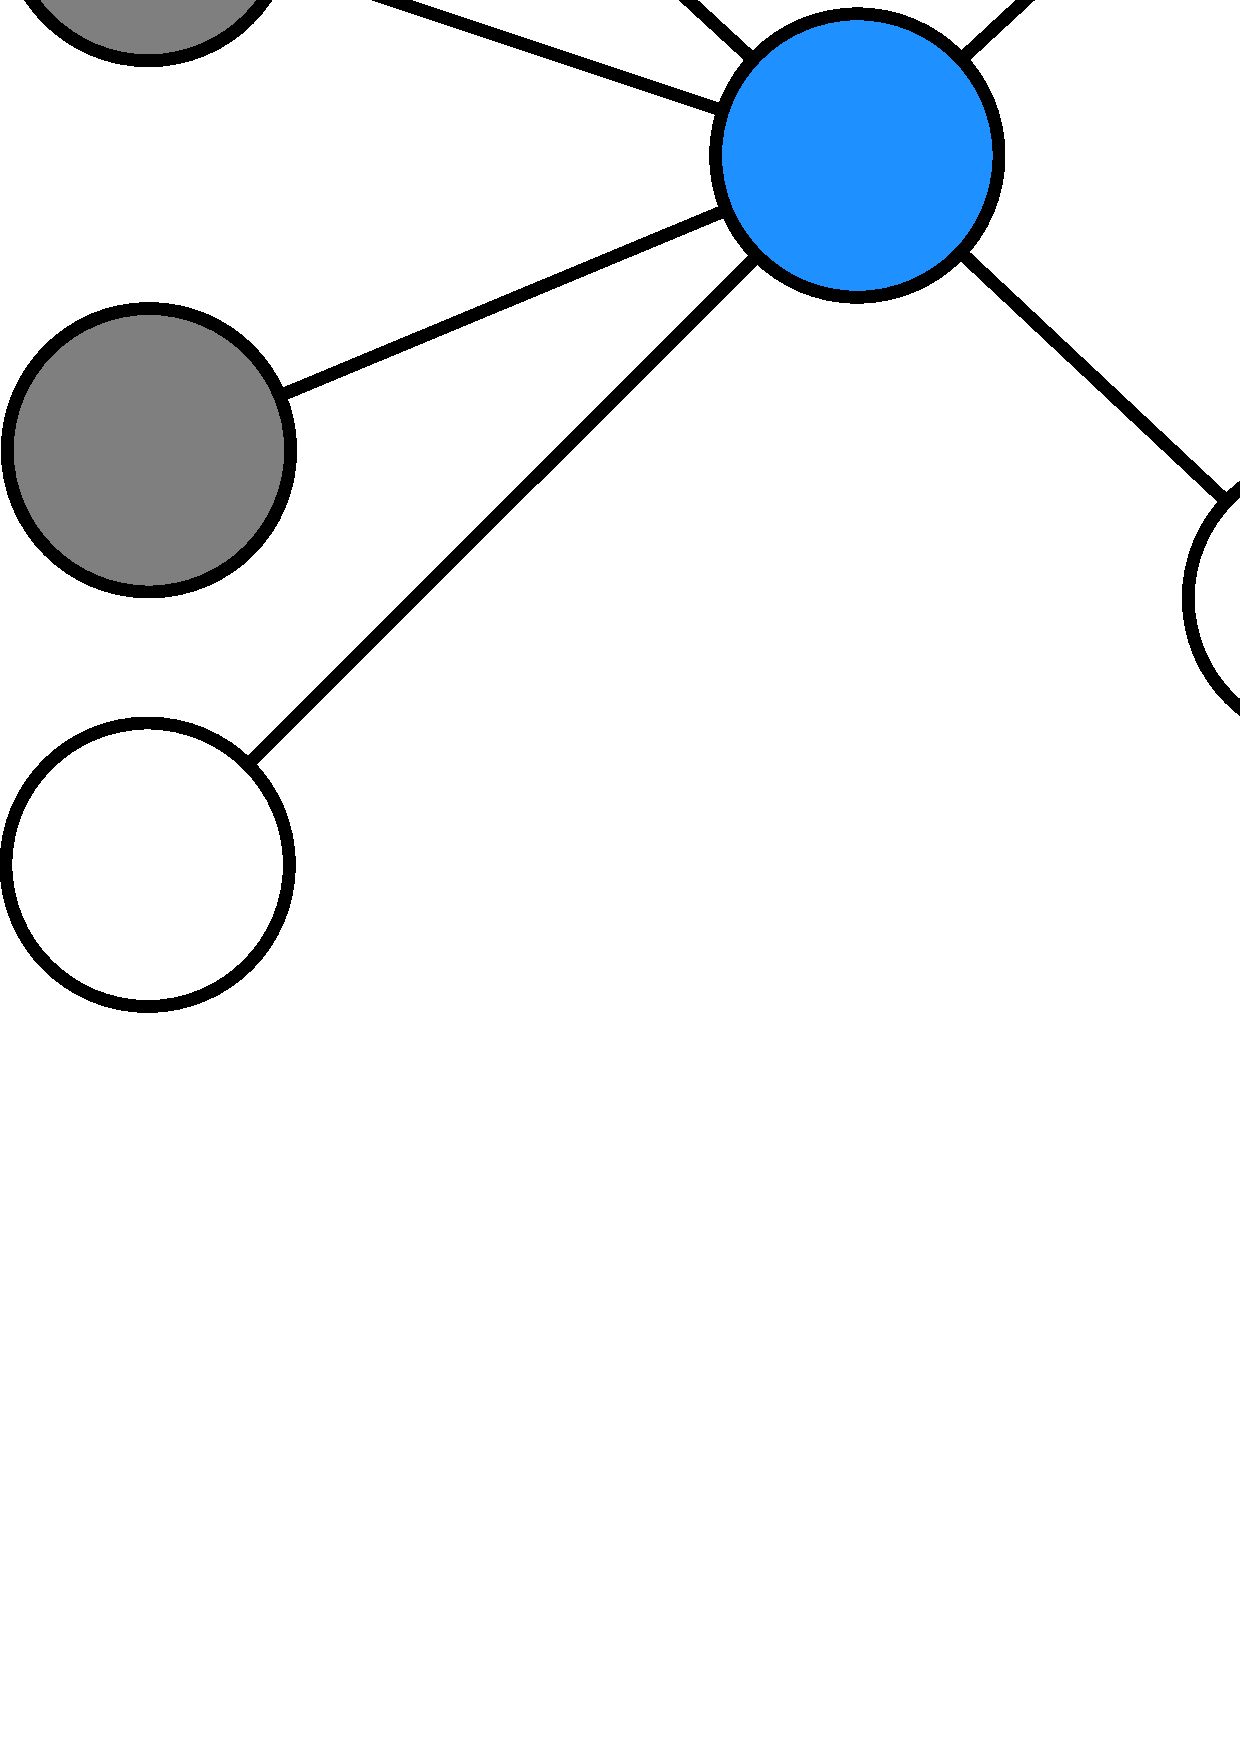
\includegraphics[width=420pt]{bilder/verschmolzenlandmarks.pdf}
   \caption{Graph $G_1$ und $G_2$ wurden verschmolzen}
  	 \end{figure}

Die metrische Dimension von diesem Graphen beträgt:

$$ \beta(G_1)+\beta(G_2)+2+r-1+ \lfloor(r-2)\times\frac{1}{3}\rfloor = \beta(G_1)+\beta(G_2)+r+2 \cdot \lfloor\frac{(r-2)}{3}\rfloor+1$$\\
Die Abbildungen \ref{bild:aussenknoten}, \ref{bild:2hintereinander} und \ref{bild:multikreise} zeigen dass es nicht möglich ist dieses Modell zu verbessern. Die außenliegenden Knoten, welche verschmolzen werden, können keine zusätzlichen Kreise bilden, da ein nicht getrenntes Knotenpaar entsteht. Das nicht getrennte Knotenpaar ist rot markiert in der Abbildung \ref{bild:aussenknoten}. 
\begin{floatingfigure}[r]{200pt}
\centering
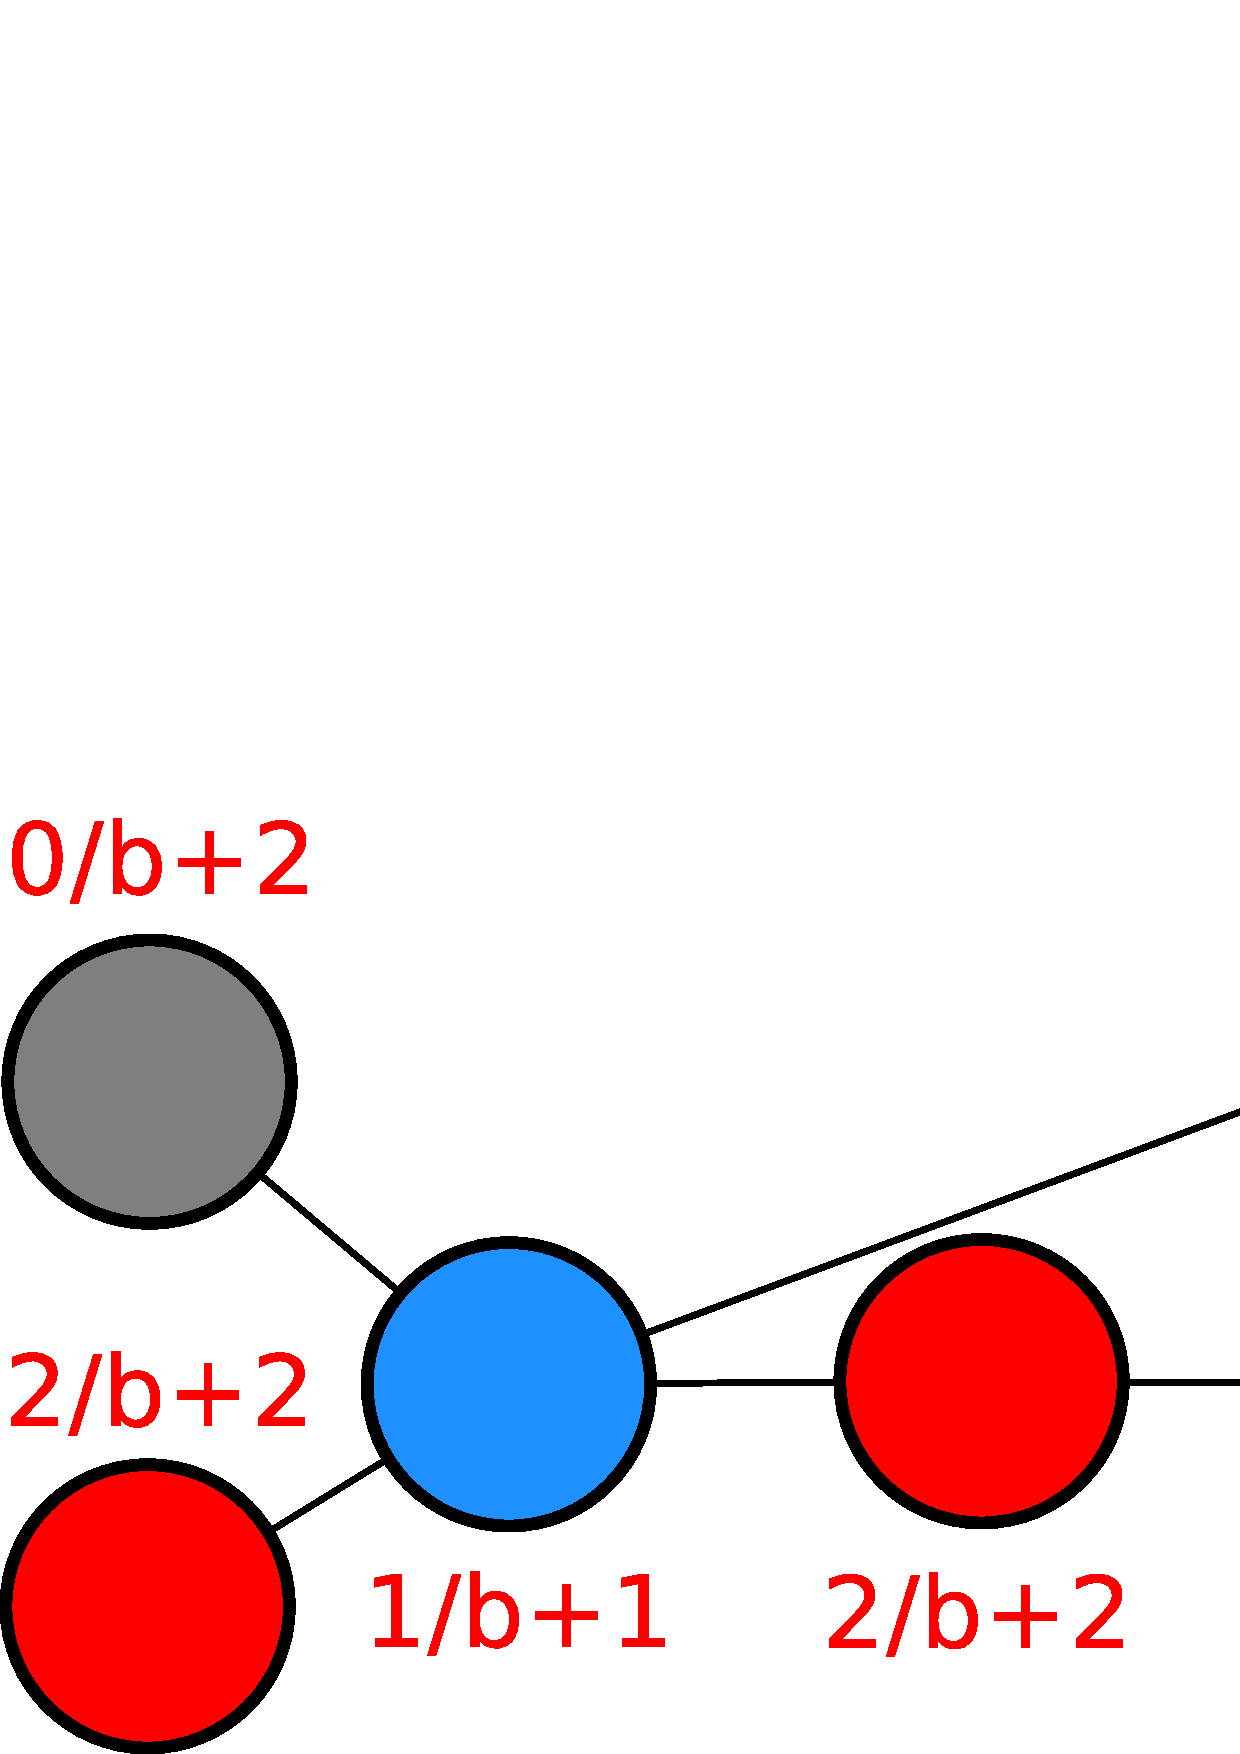
\includegraphics[width = 140pt]{bilder/gbspver1.pdf}
\caption{Gegenbeispiel für eine mögliche Verbesserung}
\label{bild:aussenknoten}
\end{floatingfigure}
Wie in der Abbildung \ref{bild:2hintereinander} dargestellt wird darf nicht jeder Knoten mit einer solchen Struktur erweitert werden. Der Versuch, weitere größere Kreise zu schaffen, scheitert schon am nächstgrößeren Beispiel, welches in der Abbildung \ref{bild:multikreise} dargestellt ist. 
\par
\vspace{+6mm}
 \begin{figure}[h!]
		\centering 		 
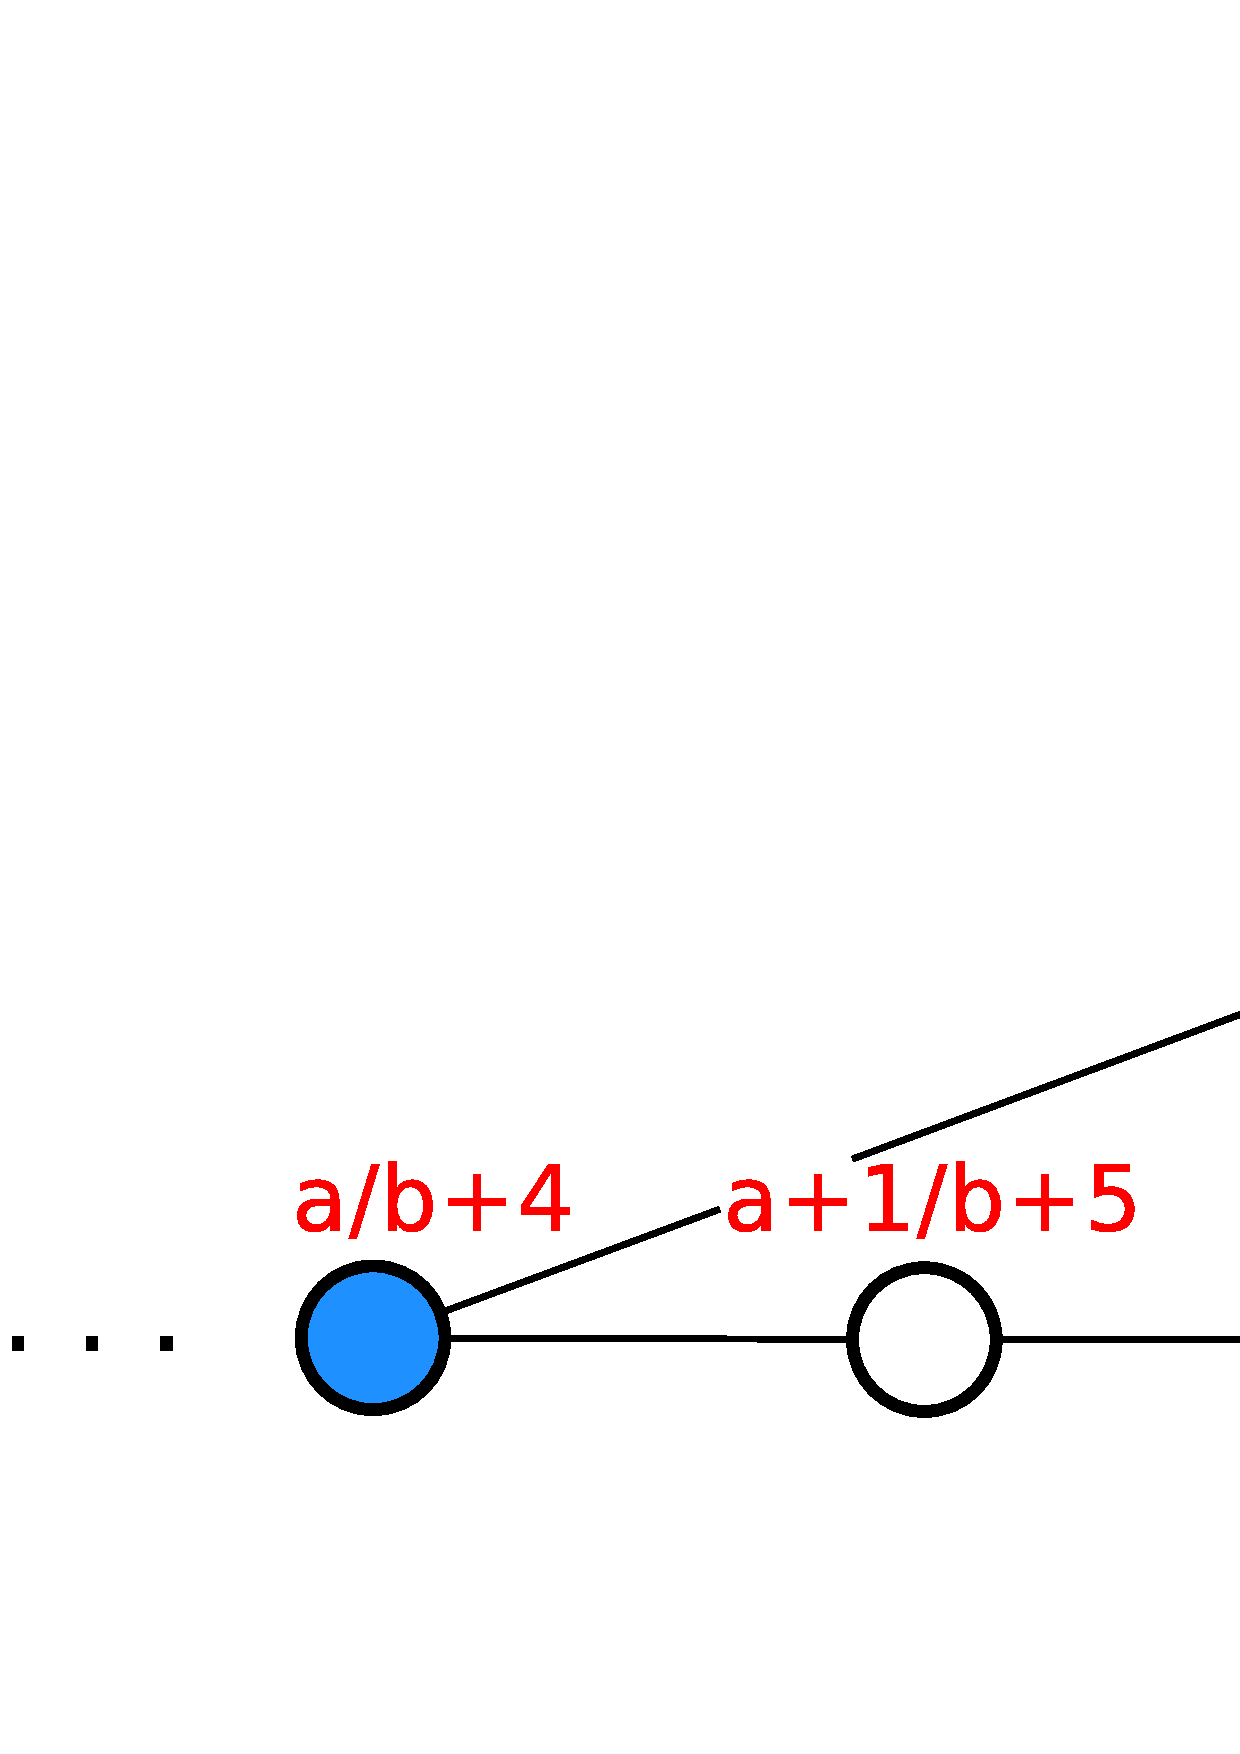
\includegraphics[width=400pt]{bilder/gbspver2.pdf}
   \caption{Gegenbeispiel für eine mögliche Verbesserung}
\label{bild:2hintereinander}  	 
  	 \end{figure}  


 \begin{figure}[h!]
		\centering 		 
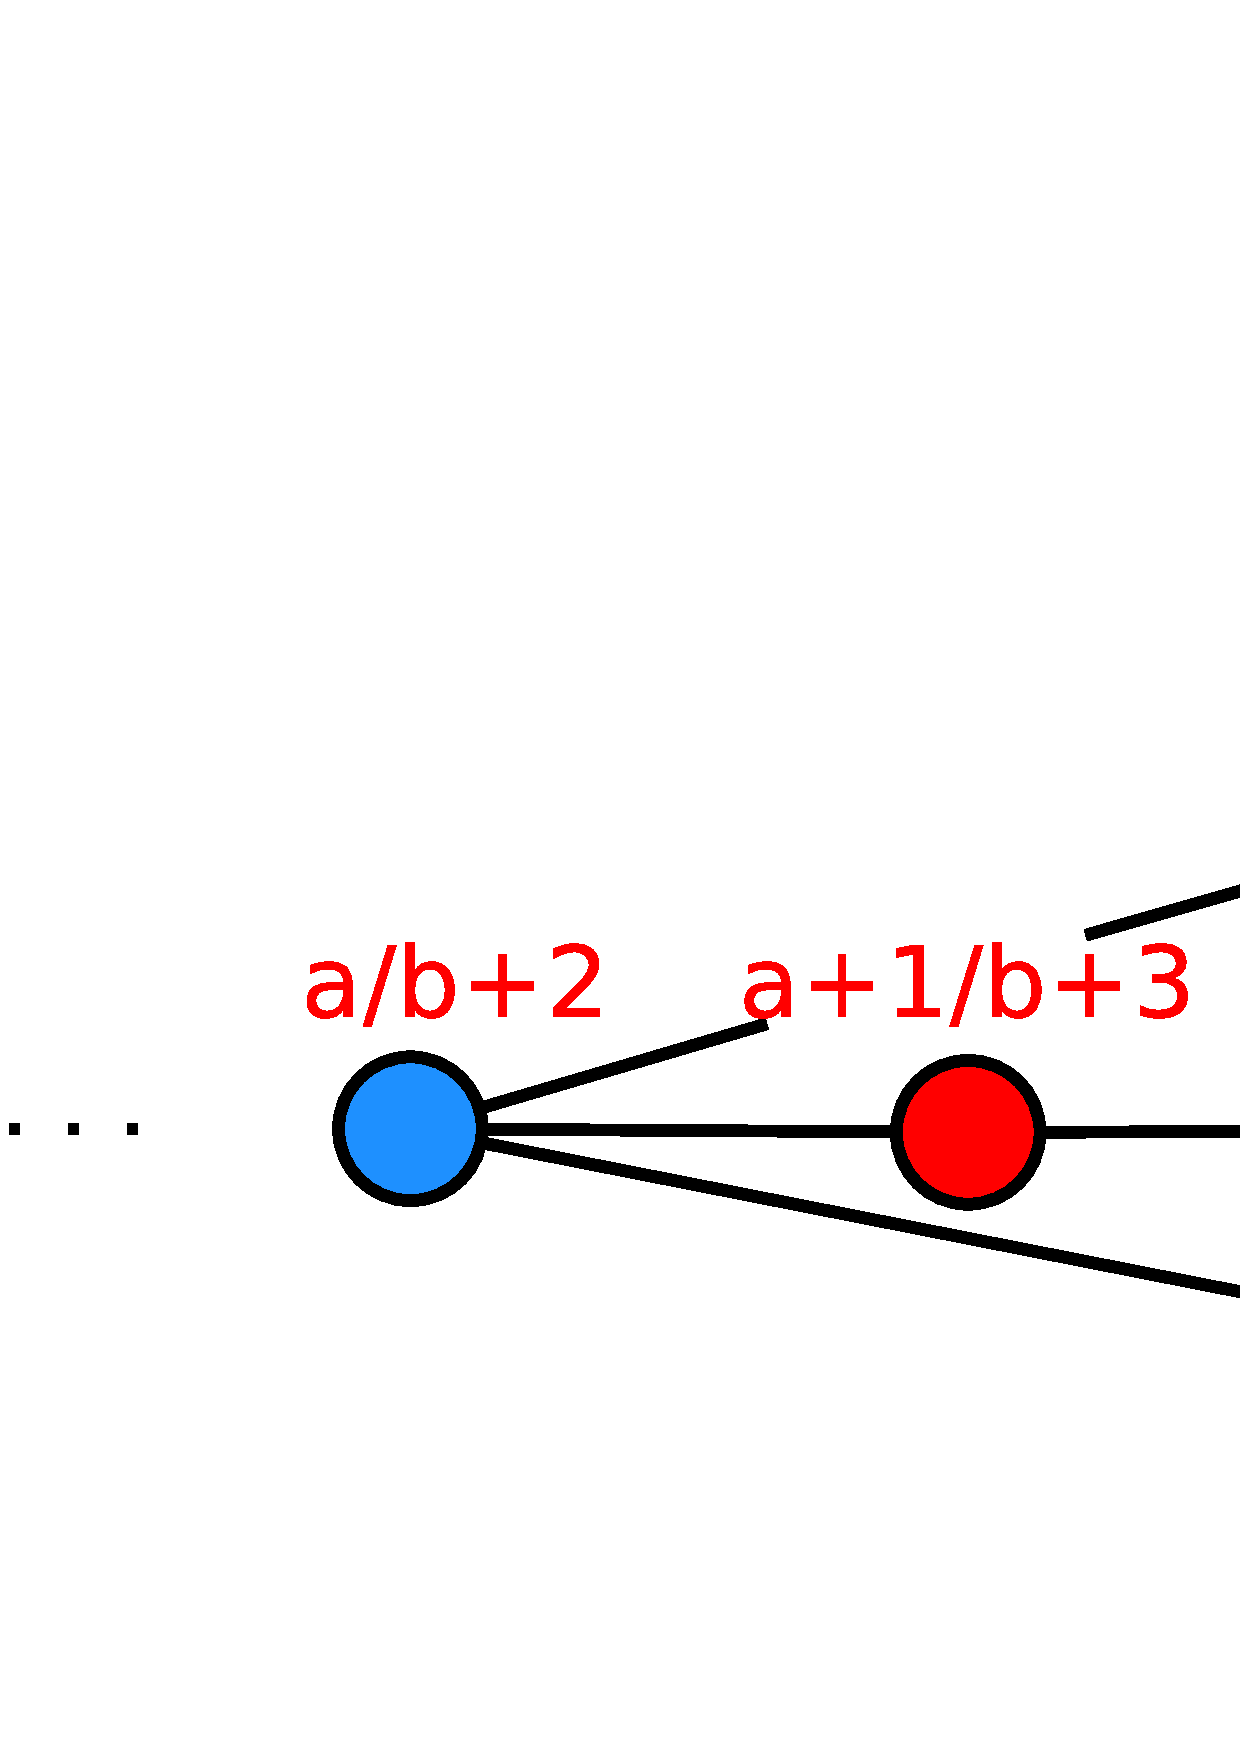
\includegraphics[width=400pt]{bilder/gbsp3.pdf}
   \caption{Gegenbeispiel für eine mögliche Verbesserung}
\label{bild:multikreise}  	 
  	 \end{figure} 
\end{proof}
\todo[inline]{1-fache Vereinigung}
%%%%%%%%%%%%%%%%%%%%%%%%%%%%%%%%%%%%%%%%%%%%%%%%%%%%%%%%%%%%%%%%%%%%%%%%%%%%%%%%%%%%%%%%%%%%%%%%%%%%%%%%%%%%%%%%%%%%%%%%%%%%%%%
\section{Zusammenhang von metrischer Dimension und Graphenstruktur}
Werden bei einem Graph Knoten oder Kanten entfernt so ist die Verkleinerung der metrischen Dimension des Graphen eine erwartete Folge. Beim Betrachten von einem vollständigen Graphen $K_n$ und dem Entfernen von Kanten bis der Graph zu einem einfachen Weg $P_n$ wird verringert sich die metrische Dimension von $n-1$ auf $1$. Dasselbe Ergebnis tritt durch das Entfernen der $n-1$ Knoten auf.\\Interessant ist die Eigenschaft, dass durch die Entfernung von Kanten die metrische Dimension auch ansteigen kann. Die folgenden Sätze zeigen, dass sich die metrische Dimension durch das Löschen von Kanten oder Knoten bei einer Graphklasse von dem konstanten Wert auf einen über die Anzahl der Knoten parametrisiertem Wert steigern kann.
%%%%%%%%%%%%%%%%%%%%%%%%%%%%%%%%%%%%%%%%%%%%%%%%%%%%%%%%%%%%%%%%%%%%%%%%%%%%%%%%%%%%%%%%%%%%%%%%%%%%%%%%%%%%%%%%%%
%%%%%%%%%%%%%%%%%%%%%%%%%%%%%%%%%%%%%%%%%%%%%%%%%%%%%%%%%%%%%%%%%%%%%%%%%%%%%%%%%%%%%%%%%%%%%%%%%%%%%%%%%%%%%%%%%%
%%%%%%%%%%%%%%%%%%%%Löschen von Knoten vergößert MD%%%%%%%%%%%%%%%%%%%%%%%%%%%%%%%%%%%%%%%%%%%%%%%%%%%%%%%%%%%%%%%
%%%%%%%%%%%%%%%%%%%%%%%%%%%%%%%%%%%%%%%%%%%%%%%%%%%%%%%%%%%%%%%%%%%%%%%%%%%%%%%%%%%%%%%%%%%%%%%%%%%%%%%%%%%%%%%%%%
%%%%%%%%%%%%%%%%%%%%%%%%%%%%%%%%%%%%%%%%%%%%%%%%%%%%%%%%%%%%%%%%%%%%%%%%%%%%%%%%%%%%%%%%%%%%%%%%%%%%%%%%%%%%%%%%%%
\subsection{Der Einfluß von Entfernung der Knoten und Kanten auf die metrische Dimension}
\begin{lem}
Die metrische Dimension eines Teilgraphen ist nicht durch die metrische Dimension des ursprünglichen Graphen beschränkt. (Durch das Entfernen von Kanten kann die metrische Dimension eines Graphen steigen.)
\end{lem}
%%%%%%%%%%%%%%%%%%%%%BEWEIS%%%%%%%%%%%%%%%%%%%%%%%%%%%%%%%%%%%%%%%%%%%%%%%%%%%%%%%%%%%%%%%%%%%%%%%%%%%%%%%%%%%%%
\begin{proof}[Beweis:]$\;$
\begin{figure}[h!]
		\centering 		 
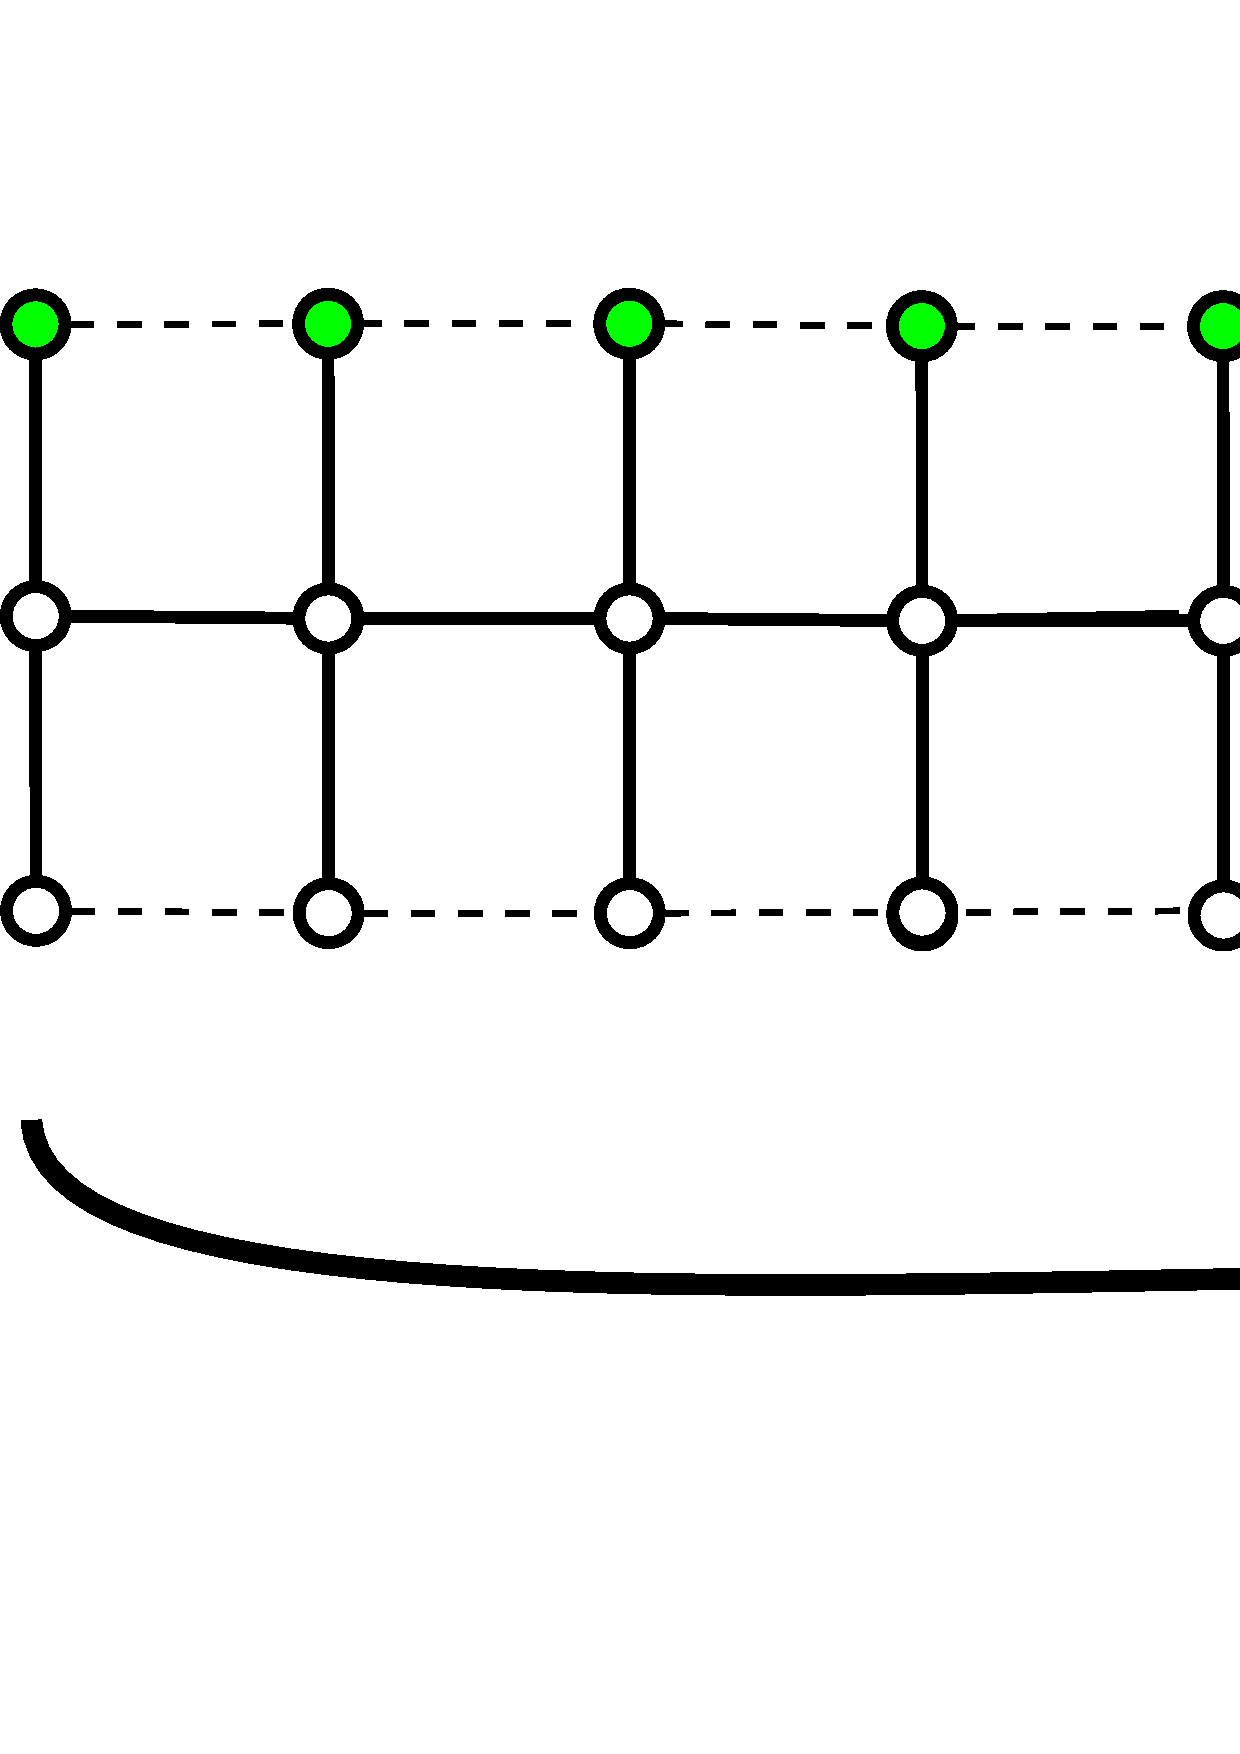
\includegraphics[width=420pt]{bilder/gitterzubaum.pdf}
   \caption{Beispiel für einen Teilgraphen mit größerer MD als der Graph selbst}
   \label{bild:Gitterbaum1}
\end{figure}
~ \linebreak
Der Gittergraph $G_{3,m}$ hat nach der Tabelle \ref{tbl:Metrische Dimension einiger Graphklassen} metrische Dimension zwei. Entfernt man alle Kanten auf dem äußeren Kreis so entsteht ein Baum $T_{3m}$ wie in Abbildung \ref{bild:Gitterbaum1} mit der metrischen Dimension $m$. Damit steigt die metrische Dimension von einem Graphen mit $n$ Knoten von zwei auf $\frac{n}{3}$.
\end{proof}
%%%%%%%%%%%%%%%%%%%%%%%%%%%%%%%%%%%%%%%%%%%%%%%%%%%%%%%%%%%%%%%%%%%%%%%%%%%%%%%%%%%%%%%%%%%%%%%%%%%%%%%%%%%%%%%%%%
%%%%%%%%%%%%%%%%%%%%%%%%%%%%%%%%%%%%%%%%%%%%%%%%%%%%%%%%%%%%%%%%%%%%%%%%%%%%%%%%%%%%%%%%%%%%%%%%%%%%%%%%%%%%%%%%%%
%%%%%%%%%%%%%%%%%%%%Löschen von Kanten vergößert MD%%%%%%%%%%%%%%%%%%%%%%%%%%%%%%%%%%%%%%%%%%%%%%%%%%%%%%%%%%%%%%%
%%%%%%%%%%%%%%%%%%%%%%%%%%%%%%%%%%%%%%%%%%%%%%%%%%%%%%%%%%%%%%%%%%%%%%%%%%%%%%%%%%%%%%%%%%%%%%%%%%%%%%%%%%%%%%%%%%
%%%%%%%%%%%%%%%%%%%%%%%%%%%%%%%%%%%%%%%%%%%%%%%%%%%%%%%%%%%%%%%%%%%%%%%%%%%%%%%%%%%%%%%%%%%%%%%%%%%%%%%%%%%%%%%%%%
\begin{lem}
Die metrische Dimension eines induzierten Teilgraphen ist nicht durch die metrische Dimension des ursprünglichen Graphen beschränkt. (Durch das Entfernen von Knoten kann die metrische Dimension eines Graphen steigen.)
\end{lem}
%%%%%%%%%%%%%%%%%%%%%BEWEIS%%%%%%%%%%%%%%%%%%%%%%%%%%%%%%%%%%%%%%%%%%%%%%%%%%%%%%%%%%%%%%%%%%%%%%%%%%%%%%%%%%%%%
\begin{proof}[Beweis:]$\;$
\begin{figure}[h!]
		\centering 		 
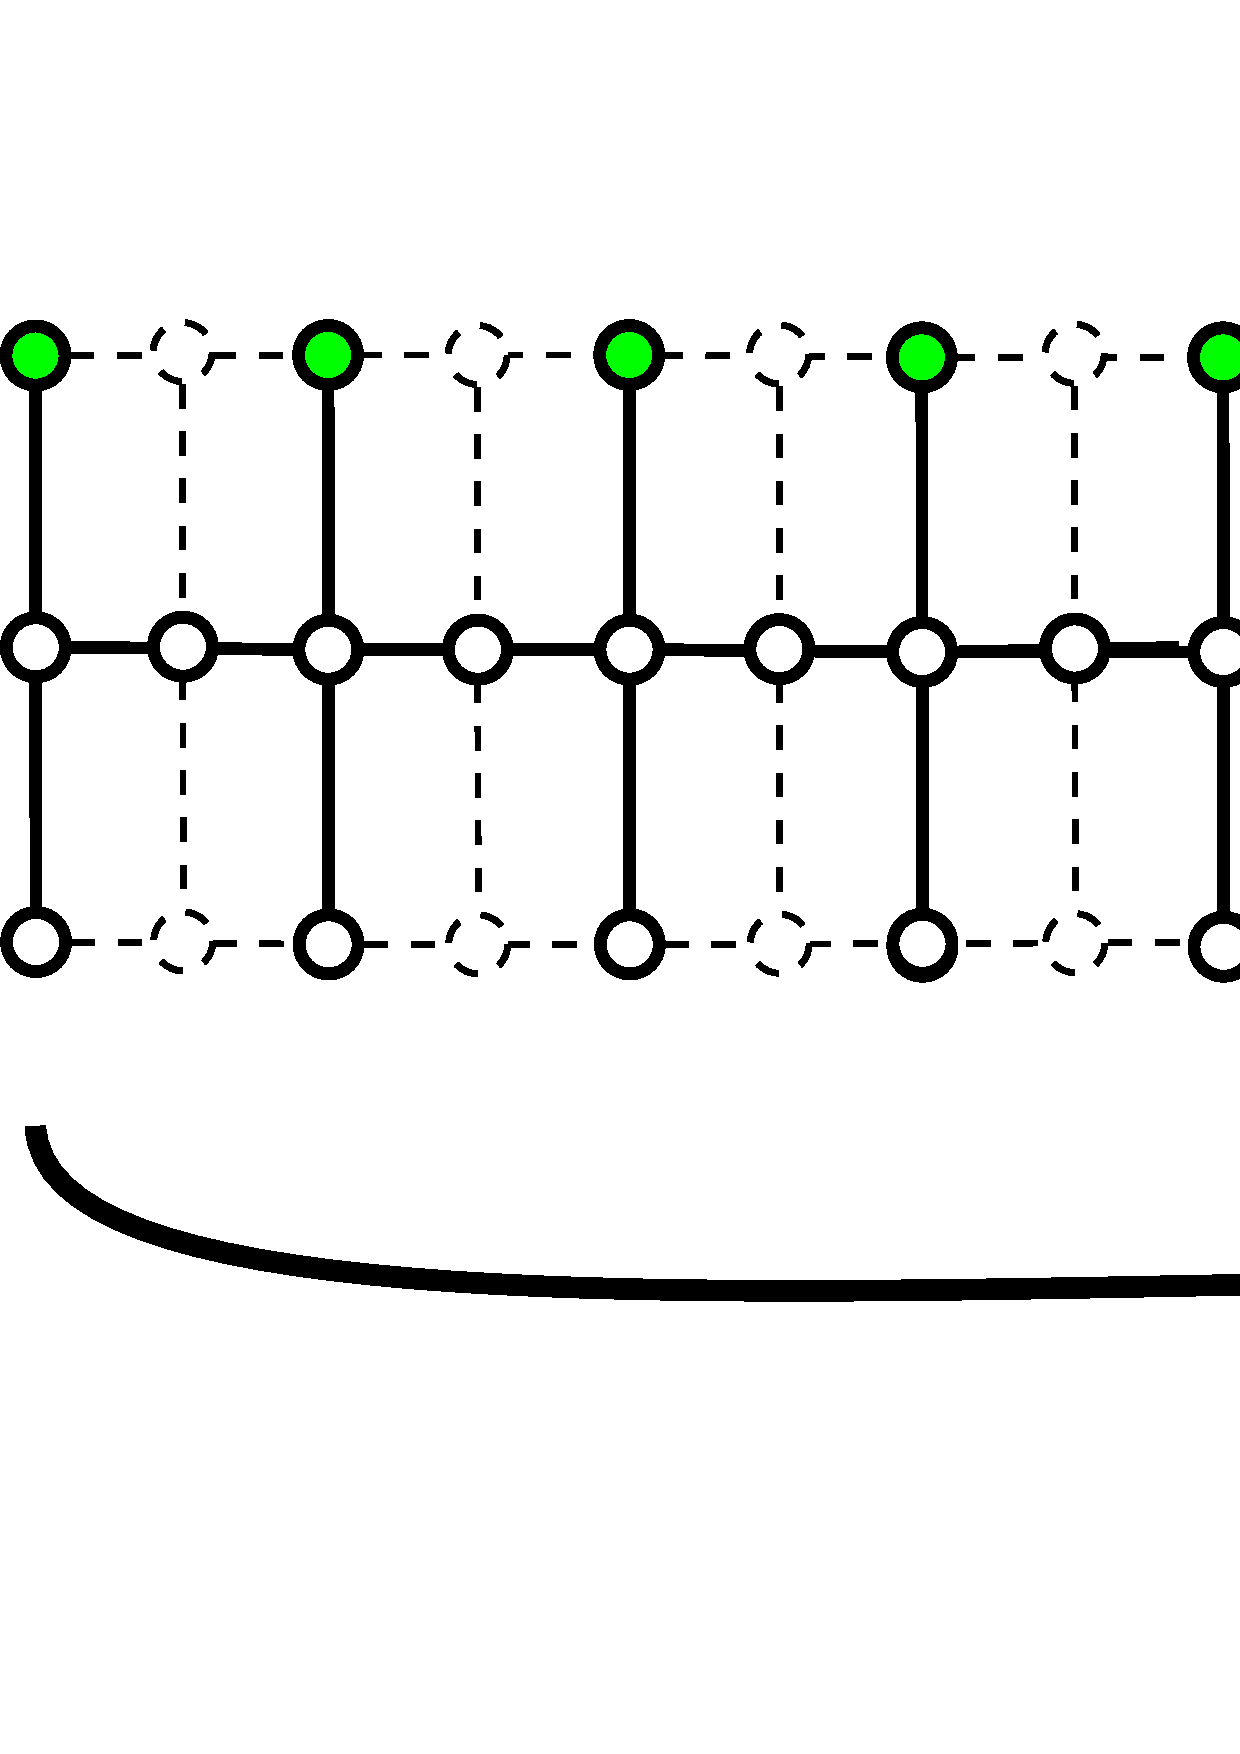
\includegraphics[width=420pt]{bilder/gitterzubaumlsch.pdf}
   \caption{Beispiel für einen induzierten Teilgraphen mit größerer MD als der Graph selbst}
   \label{bild:Gitterbaum2}
  	 \end{figure}
~ \linebreak
Der Gittergraph $G_{3,2m-1}$ hat nach der Tabelle \ref{tbl:Metrische Dimension einiger Graphklassen} metrische Dimension zwei. Entfernt man jeden zweiten Knoten auf dem äußeren Kreis so entsteht ein Baum $T_{3m}$ wie in Abbildung \ref{bild:Gitterbaum2} mit der metrischen Dimension $m$. Damit steigt der Anteil von Knoten in der metrischen Basis von $6m-3:2$ auf $3m:m$.
\end{proof}
\todo{Entfernen 1ner Kante, 1nem Knoten}

%%%%%%%%%%%%%%%%%%%%%%%%%%%%%%%%%%%%%%%%%%%%%%%%%%%%%%%%%%%%%%%%%%%%%%%%%%%%%%%%%%%%%%%%%%%%%%%%%%%%%%%%%%%%%%%%%%
%%%%%%%%%%%%%%%%%%%%%%%%%%%%%%%%%%%%%%%%%%%%%%%%%%%%%%%%%%%%%%%%%%%%%%%%%%%%%%%%%%%%%%%%%%%%%%%%%%%%%%%%%%%%%%%%%%
%%%%%%%%%%%%%%%%Zwei Teilgraphen mit je Element der MB trennen je 2 Knoten in unterschiedlichen TG %%%%%%%%%%%%%%%
%%%%%%%%%%%%%%%%%%%%%%%%%%%%%%%%%%%%%%%%%%%%%%%%%%%%%%%%%%%%%%%%%%%%%%%%%%%%%%%%%%%%%%%%%%%%%%%%%%%%%%%%%%%%%%%%%%
%%%%%%%%%%%%%%%%%%%%%%%%%%%%%%%%%%%%%%%%%%%%%%%%%%%%%%%%%%%%%%%%%%%%%%%%%%%%%%%%%%%%%%%%%%%%%%%%%%%%%%%%%%%%%%%%%%

Im Allgemeinen kann keine Kontraktion bei Wegen vorgenommen werden, aber es gibt Spezialfälle bei denen die metrische Dimension nicht verändert wird.
\clearpage
%%%%%%%%%%%%%%%%%%%%%%%%%%%%%%%%%%%%%%%%%%%%%%%%%%%%%%%%%%%%%%%%%%%%%%%%%%%%%%%%%%%%%%%%%%%%%%%%%%%%%%%%%%%%%%%%
%%%%%%%%%%%%%%%%%%%%%%%%%%%%%%%%%%%%%%%%%%%%%%%%%%%%%%%%%%%%%%%%%%%%%%%%%%%%%%%%%%%%%%%%%%%%%%%%%%%%%%%%%%%%%%%%
%%%%%%%%%%%%%%%%%%%%%%%%%%%%%%%%%%%%%%%%%%%%%%%%%%%%%%%%%%%%%%%%%%%%%%%%%%%%%%%%%%%%%%%%%%%%%%%%%%%%%%%%%%%%%%%%
\chapter{Metrische Dimension von kreisähnlichen Graphklassen}
In diesem Kapitel geht es um Graphen welche Erweiterungen von bekannten Graphklassen sind mit fester oder parameterabhängiger metrischer Dimension.\\In diesem Kapitel werden der Freundschaftsgraph und seine Verallgemeinerung, der Sonnengraph inkl. der unvollständigen Variante untersucht.
Von den verallgemeinerten Freundschaftsgraphen und den vollständigen und unvollständigen Sonnengraphen wird die metrische Dimension bestimmt unter der Vorraussetzung, dass ein Teil der metrischen Basis nicht frei gewählt werden kann. Die Resultate werden bei dem Algorithmus zur Bestimmung der metrischen Dimension von Kaktusgraphen in Kapitel \ref{kapkaktus} und bei dem Beweis der metrischen Dimension der $C_j-$Bäume in Kapitel \ref{kapcjbaume} benötigt.
\vspace{-4mm}
\section{Metrische Dimension von den Freundschaftsgraphen $F_{n}$}
''Haben je zwei Bekannte einen weiteren gemeinsamen Bekannten, so gibt es eine Person, welche alle anderen kennt''. Diese Behauptung kann als ein Graphenproblem definiert werden, wobei Knoten Personen und Kanten Bekannschaften repräsentieren. Um es zu lösen wurde von Paul Erdős et al. \cite{Erdos} der Freundschaftsgraph eingeführt. In der Arbeit von Imran et. al. \cite{Imran} wird die Partitionsdimension der Freundschaftsgraphen bestimmt und in diesem Kapitel seine metrische Dimension.
\begin{defi}{\textbf{(Freundschaftsgraph $F_{n,3}$)}}\\
Seien $n$ Kreise $C_{3}$ mit der Knotenfolge $|V|=\{v_{1,i},v_{2,i},v_{3,i}\}$  mit $1 \leq i \leq n$ gegeben. Der zweite Index steht für die Nummer des Kreises in welchem sich der Knoten befindet. Durch das Verschmelzen von allen Knoten, welche mit einer eins im ersten Index gekennzeichnet sind entsteht der Knoten $v_1$ und der Freundschaftsgraph $F_{n,3}$. Dieser Graph hat die Ordnung $2n+1$ und die Größe $3n$.
\end{defi}
\begin{bsp}~
\begin{figure}[h!]
\centering
 		 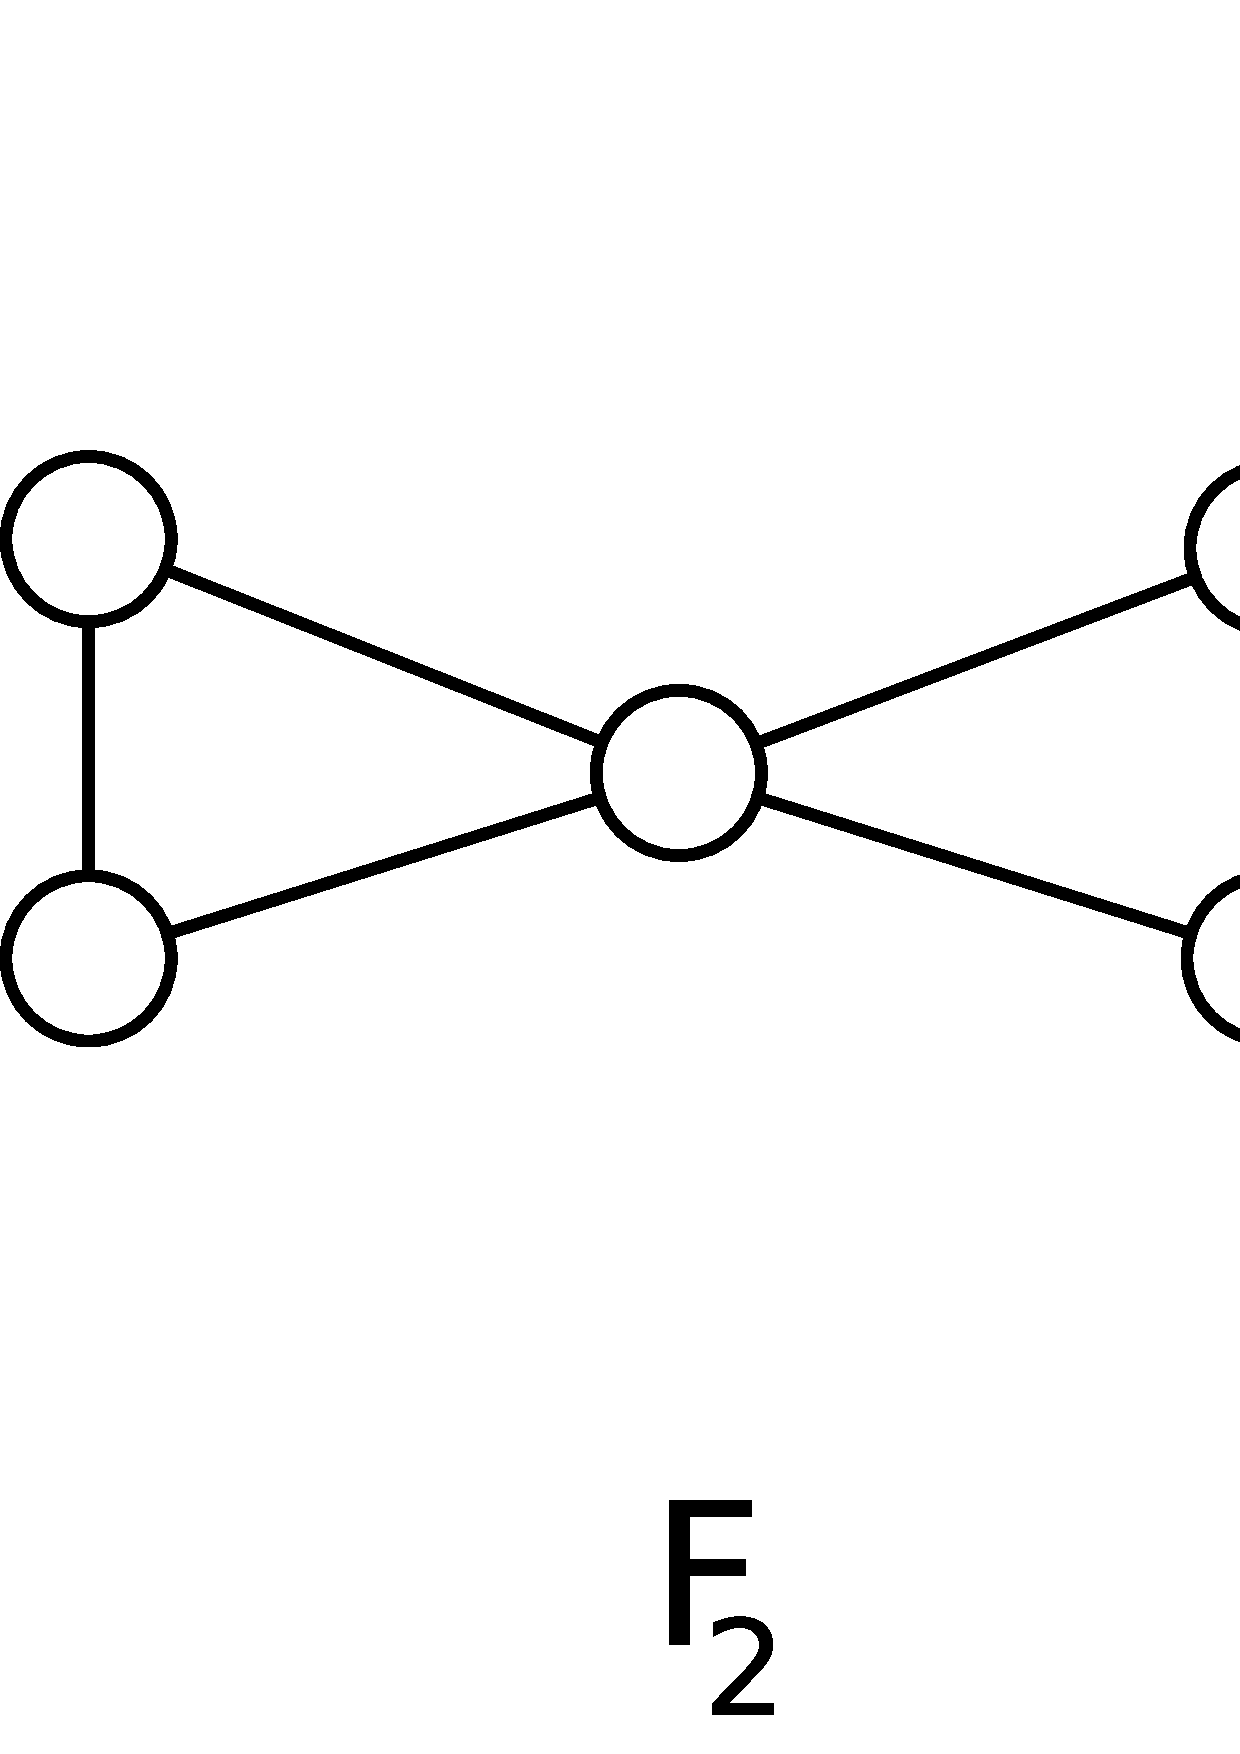
\includegraphics[width=400pt]{bilder/freunschaftsgraph.pdf}
   \caption{Vier Freundschaftsgraphen}
   \label{bild:fg}
\end{figure}
\end{bsp}
~\linebreak
\begin{lem}
\label{Freundschaftsgraphen}
Die metrische Dimension eines Freundschaftsgraphen $F_{n,3}$ ist $n$.
\end{lem}
Um diese Behauptung zu beweisen, wird das folgende Lemma benötigt. 
\begin{lem}
\label{mindfreundschaftsgraph}
Sei ein Freundschaftsgraph $F_{n,3}$ gegeben. Jede metrische Basis muss aus dem $i$-ten $C_3$ mindestens einen der folgenden Knoten $\{v_{2,i},v_{3,i}\}$ beinhalten. 
\end{lem}

\begin{proof}[Beweis:]~
\par
\begin{floatingfigure}[l]{200pt}
{\flushleft
\hspace*{1.7cm}
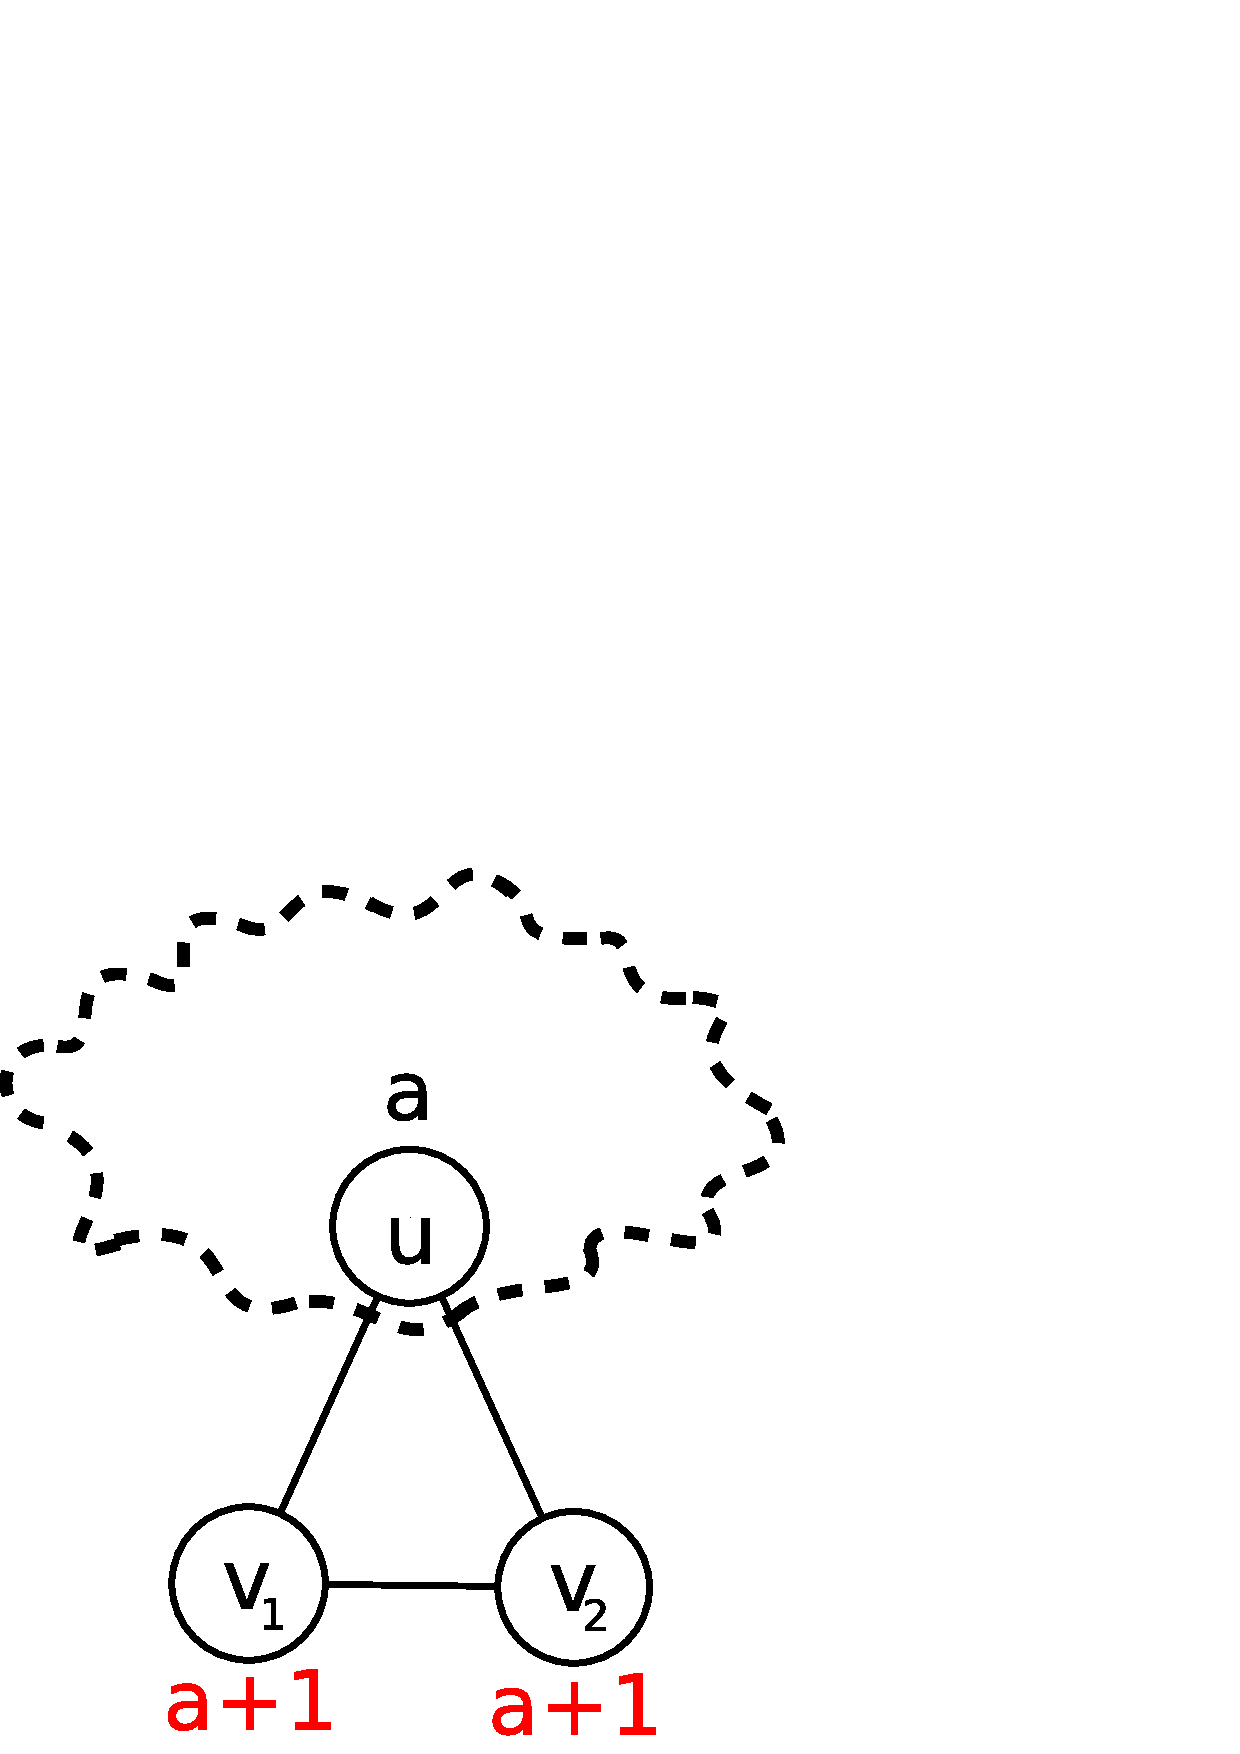
\includegraphics[width=100pt]{bilder/freundschaftsgraphbew.pdf}}
\caption{Ein markierter $C_{3}$}
\label{CA9}
\end{floatingfigure}

Angenommen es gibt einen $C_3$ bei\\welchem keiner dieser Knoten in\\der metrischen Basis ist.\\Durch die eindeutige Verbindung zu dem Restgraphen, welche über einen\\Trennungsknoten läuft, folgt aus\\Symmetriegründen, dass die Knoten $v_{2,i}$\\und $v_{3,i}$ identische Markierungen haben.\\Dies ist ein Widerspruch zu der\\Definition einer metrischen Basis.\\
Die metrische Dimension eines Freundschaftsgraphen $F_{n,3}$ ist mindestens gleich der Anzahl seiner $C_{3}$, mindestens $n$.
\end{proof}
\par
\vspace{-6mm}
\begin{proof}[Beweis von Lemma \ref{Freundschaftsgraphen}:] \vspace{+1mm} ~ \linebreak
Nach Lemma \ref{mindfreundschaftsgraph} ist bekannt, dass die metrische Dimension eines Freundschaftsgraphen $F_{n,3}$ mindestens $n$ ist. Angenommen, alle als $v_{2,i}$ markierten Knoten werden in die metrische Basis aufgenommen. Also sind sie getrennt. Der Knoten $v_1$ hat die Distanz eins zu allen Knoten in der metrischen Basis und ist der einzige Knoten mit dieser Eigenschaft. Für jeden Knoten $v_{3,i}$ gibt es genau einen Knoten $v_{2,i}$ mit der Distanz eins. Zu allen anderen Knoten in der metrischen Basis hat jeder Knoten $v_{3,i}$ die Distanz zwei. Alle Markierungen sind eindeutig und der gesamte Graph ist durch die $n$ Knoten getrennt.
\end{proof}
\vspace{-12mm}
~ \linebreak

Werden nicht nur Kreise der Länge drei sondern beliebiger Länge betrachtet bleibt die metrische Dimension des $F_{n,k}$ für $k=2j+1$, $j\geq 2$ erhalten und für $k=2j$, $j\geq 2$ vergrößert sie sich um $n-1$.
\begin{defi}{\textbf{(Verallgemeinerter Freundschaftsgraph $F_{n,k}$)}}\\
Seien $n$ Kreise $C_k=(V_k,E_k)$ mit der Knotenfolge $|V_k|=\{v_{1,i},\ldots,v_{k,i}\}$ gegeben. Durch das Verschmelzen von allen Knoten, welche mit einer eins im ersten Index gekennzeichnet sind, entsteht der Knoten $v_1$ und der Freundschaftsgraph $F_{n,k}$. Dieser Graph hat die Ordnung $kn+1$ und die Größe $kn$.
\end{defi}

\begin{lem}
\label{verallgFreundschaftsgraphen}
Die metrische Dimension eines Freundschaftsgraphen $F_{n,k}$ mit $k=2j+1$ für $j \geq 1$ ist $n$ und die metrische Dimension eines Freundschaftsgraphen $F_{n,k}$ mit $k=2j$ für $j \geq 2$ ist $2n-1$.
\end{lem}
\begin{lem}
\label{mindverallgfreundschaftsgraph}
Sei ein Freundschaftsgraph $F_{n,k}$ gegeben. Jede metrische Basis muss aus dem $i$-ten $C_k$ mindestens einen der folgenden Knoten $\{v_{2,i},\ldots,v_{k,i}\}$ beinhalten.
\end{lem}
\begin{proof}[Beweis:]
Angenommen, aus dem $i$-ten Kreis $C_k$ ist keiner dieser Knoten in der metrischen Basis. Durch die eindeutige Verbindung zu dem Restgraphen, welche über einen Trennungsknoten läuft, folgt aus Symmetriegründen, dass die Knoten $v_{2,i}$ und $v_{k,i}$ identische Markierungen haben.\\Dies ist ein Widerspruch zu der Definition einer metrischen Basis.\\
Damit ist die metrische Dimension eines Freundschaftsgraphen $F_{n,k}$ mindestens gleich der Anzahl seiner $C_{k}$ und damit mindestens $n$.
\end{proof}
\vspace{-6mm}
\begin{proof}[Beweis von Lemma \ref{verallgFreundschaftsgraphen} für $k=2j+1$:] \vspace{+1mm} ~ \linebreak 
Nach Lemma \ref{mindverallgfreundschaftsgraph} ist bekannt, dass die metrische Dimension eines Freundschaftsgraphen $F_{n,k}$ mindestens $n$ ist. Angenommen, alle als $v_{\lceil \frac{n}{2} \rceil}$ markierten Knoten werden in die metrische Basis aufgenommen. Dadurch sind sie getrennt. Jeder Knoten $v_i$ auf dem jeweiligen Kreis hat die Distanz $\leq \lfloor \frac{n}{2} \rfloor$ zu dem Knoten $v_{\lceil \frac{n}{2} \rceil}$ und die Distanz $\geq \lfloor \frac{n}{2} \rfloor$ zu allen Knoten in der metrischen Basis. Der Knoten $v_1$ hat als einziger Knoten die Distanz $\lfloor \frac{n}{2} \rfloor$ zu allen Anderen. Jeder andere Knoten ist nach den Sätzen \ref{tbl:Metrische Dimension einiger Graphklassen} und \ref{} getrennt.
\end{proof}
\begin{proof}[Beweis von Lemma \ref{verallgFreundschaftsgraphen} für $k=2j$:] \vspace{+1mm} ~ \linebreak 
Nach Lemma \ref{mindverallgfreundschaftsgraph} ist bekannt, dass die metrische Dimension eines Freundschaftsgraphen $F_{n,k}$ mindestens $n$ ist. \todo{Beweis auschreiben}
\end{proof}
\begin{lem}
Die metrische Dimension von allgemeinen Freundschaftgraphen $F_{n}$ mit unterschiedlicher Kreislänge ist $n+n_g-1$. Dabei ist $n=n_u+n_g$ und $n_u$ ist die Anzahl der Kreise mit ungerader Länge und $n_g$ die Anzahl der Kreise mit gerader Länge.
\end{lem}
\subsection{Metrische Dimension von allgemeinen Freundschaftgraphen und Bäumen}
%%%%%%%%%%%%%%%%%%%%%%%%%%%%%%%%%%%%%%%%%%%%%%%%%%%%%%%%%%%%%%%%%%%%%%%%%%%%%%%%%%%%%%%%%%%%%%%%%%%%%%%%%%%%%%%%
\newpage
\section{Metrische Dimension der Sonnengraphen $S_{n,k}$}
Trotz vieler Literatur über die metrische Dimension wurde bis jetzt die metrische Dimension von Kreisen, welche an manchen Knoten Wege besitzen nicht betrachtet. Lediglich ein Spezialfall und zwar der Drachengraphen \cite{blabla}, wo ein Kreis mit einem Weg durch eine Kante an einen Endknoten des Weges vereinigt wird, wurde analysiert und die metrische Dimension davon ist zwei. Diese Graphklassen ist sehr wichtig für diese Arbeit, denn die Sonnengraphen sind induzierte Teilgraphen von in dem Kapitel \ref{kapcjbaume} behandelten $C_j$-Bäumen und in dem Kapitel \ref{kapkaktus} behandelten Kaktusgraphen.
\begin{defi}{\textbf{(Sonnengraph $S_{n,k}$)}}\\
Sei ein Kreis $C_n$ für $n \geq 3$ mit der Knotenmenge $|V|=\{ c_1, \ldots , c_n \}$ und $n$ Weggraphen $P_{k-1}$ für $k \geq 2$ gegeben. Die Knoten mit Grad eins auf dem $i-$ten Weg werden als $v_{i,1}$ und $v_{i,k-1}$ bezeichnet. Durch das Hinzufügen von $n$ neuen Kanten der Form $\{v_{i,1},c_i\}$ für $1 \leq i \leq n$ ensteht der zusammenhängende Sonnengraph $S_{n,k}$.\\
Alle als $v_{i,k-1}$ bezeichneten Knoten werden Endknoten genannt, als $c_i$ bezeichneten Knoten werden Ursprungsknoten genannt und eine Knotenmenge mit den\\Knoten $\{c_i,v_{i,1}, \ldots ,v_{i,k-1}\}$ für $1 \leq i \leq n$ als Strahl. (vgl. Abbildung \ref{bild:sonnengraph})\\
Für $n=1$ ist der Graph der Sterngraph aus Definition \ref{defstern}. Als Sonnengraph $S_n$ bezeichnet man einen Graphen mit $n$ Strahlen beliebiger Länge $i$ mit $i \geq 2$.
\end{defi}
\begin{figure}[h!]
\centering
 		 \includegraphics[width=165pt]{bilder/sonne4.pdf}
   \caption{Der Sonnengraph $S_{12,3}$}
   \label{bild:sonnengraph}
\end{figure}
%\begin{bem}
%Nach Satz \ref{sepvertex} können beliebige Wege $P_i$ mit $i\geq 2$ bei der Berechnung der metrischen Dimension als $P_2$ aufgefasst werden. Also gilt: $$md(S_{n,2})=md(S_{n,3})= \ldots =md(S_{n,k})=md(S_{n})$$
%Im folgenden wird der Graph $S_{n,2}$ repräsentativ für $S_{n,k}$ betrachtet.
%\end{bem}
\begin{lem}
Die metrische Dimension eines Sonnengraphen $S_{n,k}$ mit $n=4$ und $n = 2j+1$ für $j \in \mathbb{N}$ ist zwei und die metrische Dimension eines Sonnengraphen $S_{n,k}$ mit $n = 2j+4$ für $j \in \mathbb{N}$ ist drei.
\end{lem}
\begin{figure}[h!]
\begin{minipage}[hbt]{7cm}
	\centering
	\includegraphics[width=190pt]{bilder/sonne4k.pdf}  
   \caption{Der Sonnengraph $S_{4,2}$}  
	\label{Bild1}
\end{minipage}
\hfill
\begin{minipage}[hbt]{7cm}
	\centering
	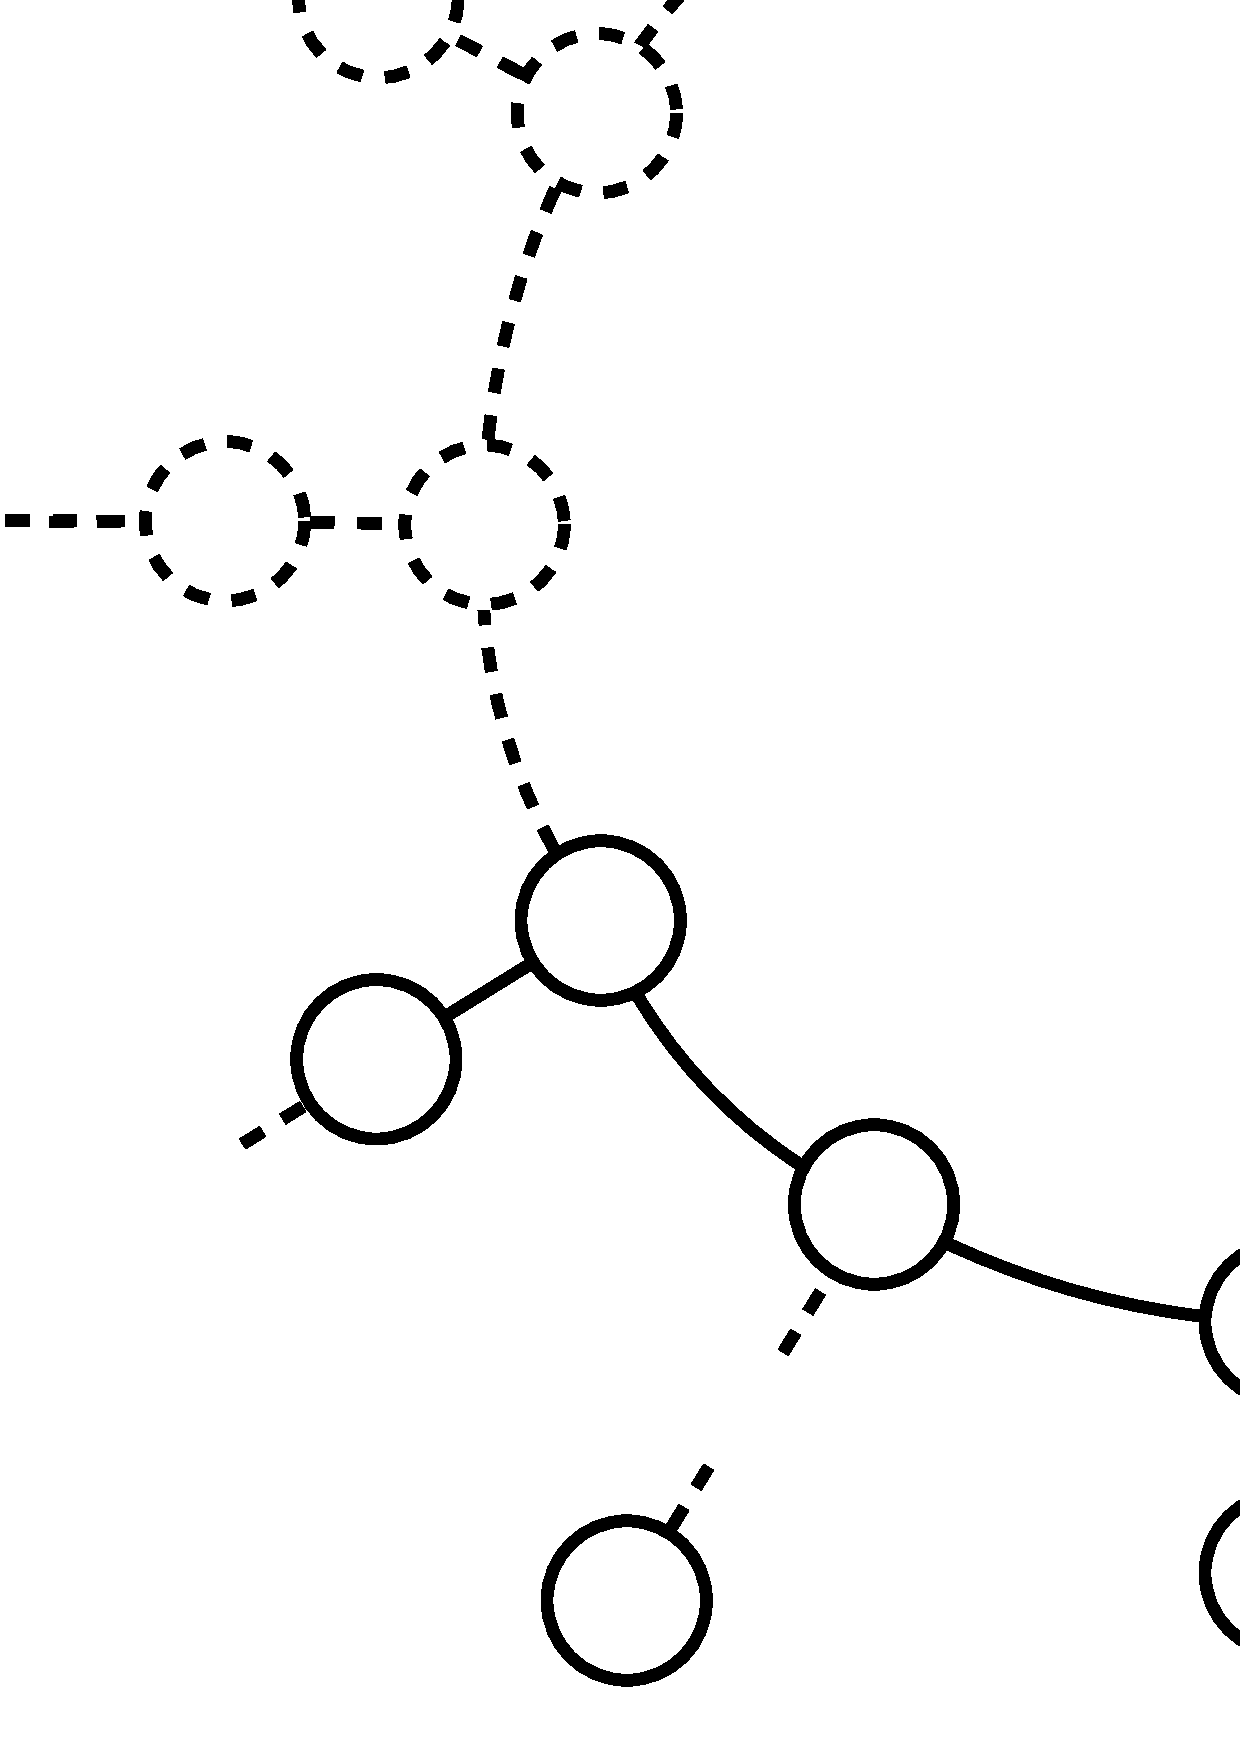
\includegraphics[width=190pt]{bilder/sonne2.pdf}
   \caption{Der Sonnengraph $S_{2n,2}$}
	\label{Bild2}
\end{minipage}
\end{figure}
\begin{lem}
Die metrische Dimension eines Sonnengraphen $S_{n,k}$ mit $n = 2j+4$ für $j \in \mathbb{N}$ kann nicht zwei sein. 
\end{lem}
\begin{proof}[Beweis:]
Für den ersten Knoten in der metrischen Basis gibt es $(k-1)\cdot n$ Möglichkeiten, aber nur $n$ unterschiedliche Fälle. Denn wird der erste Knoten aus einem Strahl aufgenommen, so gilt nach Lemma \ref{}, dass der Strahlursprung als Element der metrischen Basis betrachtet werden kann. Der zweite Knoten muss die Bedingung vom Lemma \ref{Bifurnachbar} erfüllen.  
 \begin{figure}[h!]
		\centering
 		 \includegraphics[width=100pt]{bilder/gbsbspsonne2glr.pdf}
   \caption{Ein $C_{n}-Blatt$ mit zwei Knoten in der metrischen Basis, welche die Bedingung aus Lemma \ref{Bifurnachbar} erfüllen}
  	 \end{figure}
  	  	 
Es bleiben noch genau drei Möglichkeiten $v_{\frac{n}{2}}$,$v_{\frac{n-1}{2}}$ und $v_{\frac{n+1}{2}}$.\\ 
Der Knoten $v_{\frac{n}{2}}$ kann nicht aufgenommen werden, da zwei gegenüberliegende Knoten einen Kreis gerader Länge nicht trennen \cite{}.\\
Durch die Wahl von $v_{\frac{n-1}{2}}$ oder $v_{\frac{n+1}{2}}$ entstehen mindestens zwei Markierungen der Form $a/b$ und $a+1/b+1$ auf dem Kreis. Da jeder Knoten ein Strahlursprung ist, gibt es in dem Graphen einen weiteren Knoten mit der Markierung $a+1/b+1$. Zur Veranschaulichung wird der Graph $S_{6,2}$ betrachtet.
\begin{figure}[h!]
		\centering
 		 \includegraphics[width=100pt]{bilder/bspsonne6.pdf}
   \caption{Ein markierter $S_{6,2}$ mit zwei Knoten in der MB}
  	 \end{figure}
\end{proof}
\begin{proof}[Beweis:]
%\begin{figure}[h!]
%		\centering
% 		 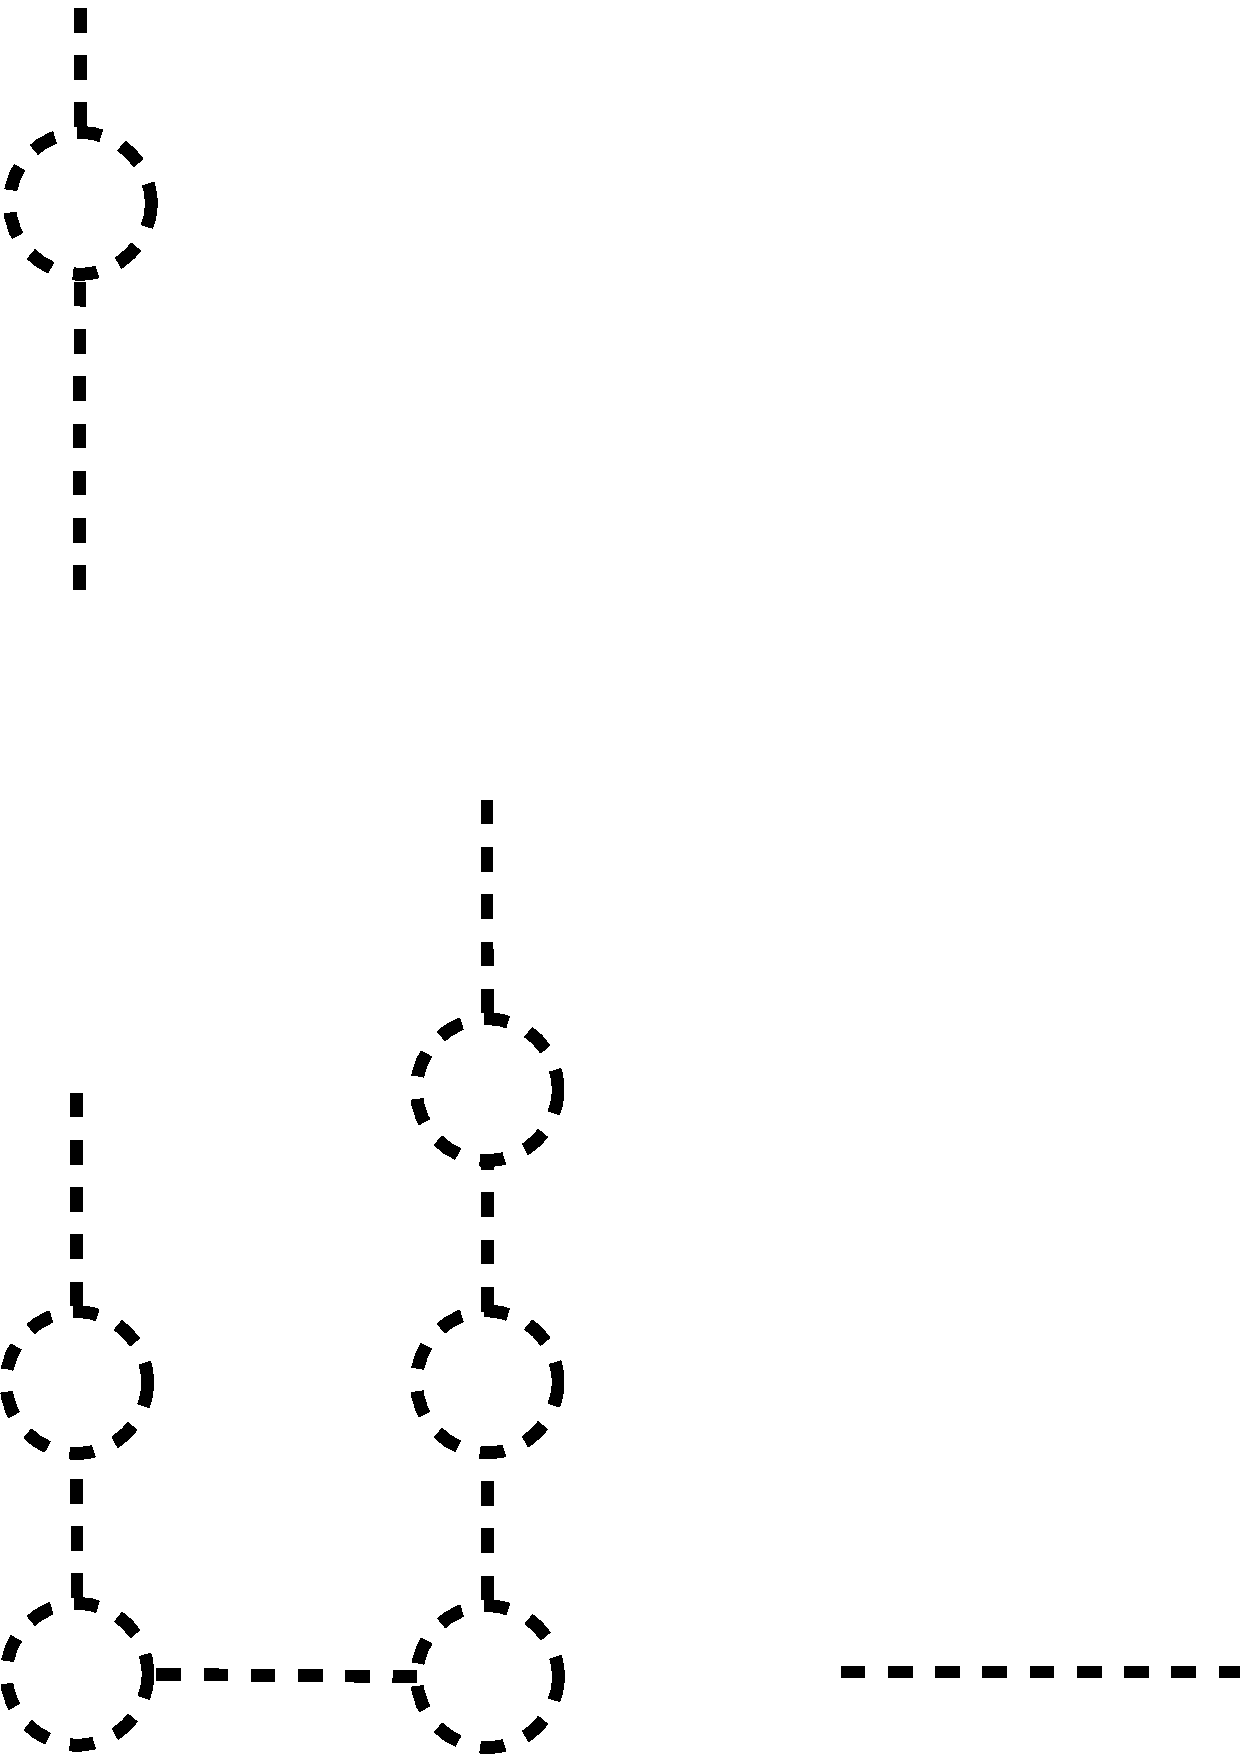
\includegraphics[width=430pt]{bilder/sonne1.pdf}
%   \caption{Ein $C_{n}-Blatt$ wird durch zwei Knoten getrennt}
%  	 \end{figure}
Jeder Knoten auf einem Strahl hat eine $a+x/b+x$ Markierung mit $0 \leq x \leq k$ und $a/b$ die Markierung des Strahlursprung auf dem Kreis $C_n$.
\end{proof}
\subsection{Metrische Dimension unvollständiger Sonnengraphen}  	 
\begin{defi}{\textbf{(Unvollstängiger Sonnengraph $S'_{n,k}$)}}\\
Sei ein Kreis $C_n$ für $n \geq 3$ mit der Knotenmenge $|V|=\{ c_1, \ldots , c_n \}$ und $n'$ Weggraphen $P_{k'}$ mit $1 \leq n' \leq n-1$ für $2 \leq k' \leq k$ gegeben. Die Knoten mit Grad eins auf dem $i-$ten Weg werden als $v_{i,1}$ und $v_{i,k-1}$ bezeichnet. Durch das Hinzufügen von $n'$ neuen Kanten der Form $\{v_{i,1},c_i\}$ für $1 \leq i \leq n$ ensteht der zusammenhängende Sonnengraph $S'_{n',k'}$. Knoten mit den Indizes $v_{i,k-1}$ werden Endknoten genannt und Knoten mit der Bezeichnung $c_i$ als Ursprungsknoten. Die Knotenmenge mit den Knoten $\{c_i,v_{i,1}, \ldots ,v_{i,k-1}\}$ für $1 \leq i \leq n$ bezeichnet man als Strahl. (vgl. Abbildung \ref{bild:sonnengraph})
\end{defi}
\begin{satz}
\label{schrankenunvsg}
Für die metrische Dimension eines unvollständigen Sonnengraphen $S'_{n,k}$ gilt:
$$\beta(C_n) \leq \beta(S'_{n,k})\leq \beta(S_{n,k})$$
\end{satz}
\begin{proof}
\end{proof}
\begin{bem}
Nach Satz \ref{schrankenunvsg} gilt für $n=2k+1$ für $k \in \mathbb{N}$: $$2=\beta(C_n) \leq \beta(S'_{n,k})\leq \beta(S_{n,k})=2$$
Daraus folgt, dass die metrische Dimension eines unvollständigen Sonnengraphen $S'_{n,k}$ mit $n=2k+1$ für $k \in \mathbb{N}$ zwei ist.\\
Für die metrische Dimension für $n=2k+2$ für $k \in \mathbb{N}$ gilt: $$2=\beta(C_n) \leq \beta(S'_{n,k})\leq \beta(S_{n,k})=3$$
Daraus folgt, dass die metrische Dimension eines unvollständigen Sonnengraphen $S'_{n,k}$ mit $n=2k+2$ für $k \in \mathbb{N}$ entweder zwei oder drei ist. Um die metrische Dimension genau zu bestimmen werden $\frac{n}{2}$ unterschiedliche Fälle betrachtet.
\end{bem}
\begin{table}[htp]
\centering
 \renewcommand{\arraystretch}{2}
\begin{tabularx}{\textwidth}{||c|c||}
\hline\hline
\vspace{0.3mm}
1. Fall& \multirow{3}{121mm}{$\frac{n}{2}-2$ benachbarte Knoten ohne Strahlen}\\
\cline{1-1}
\vspace{-6mm}
&\\
	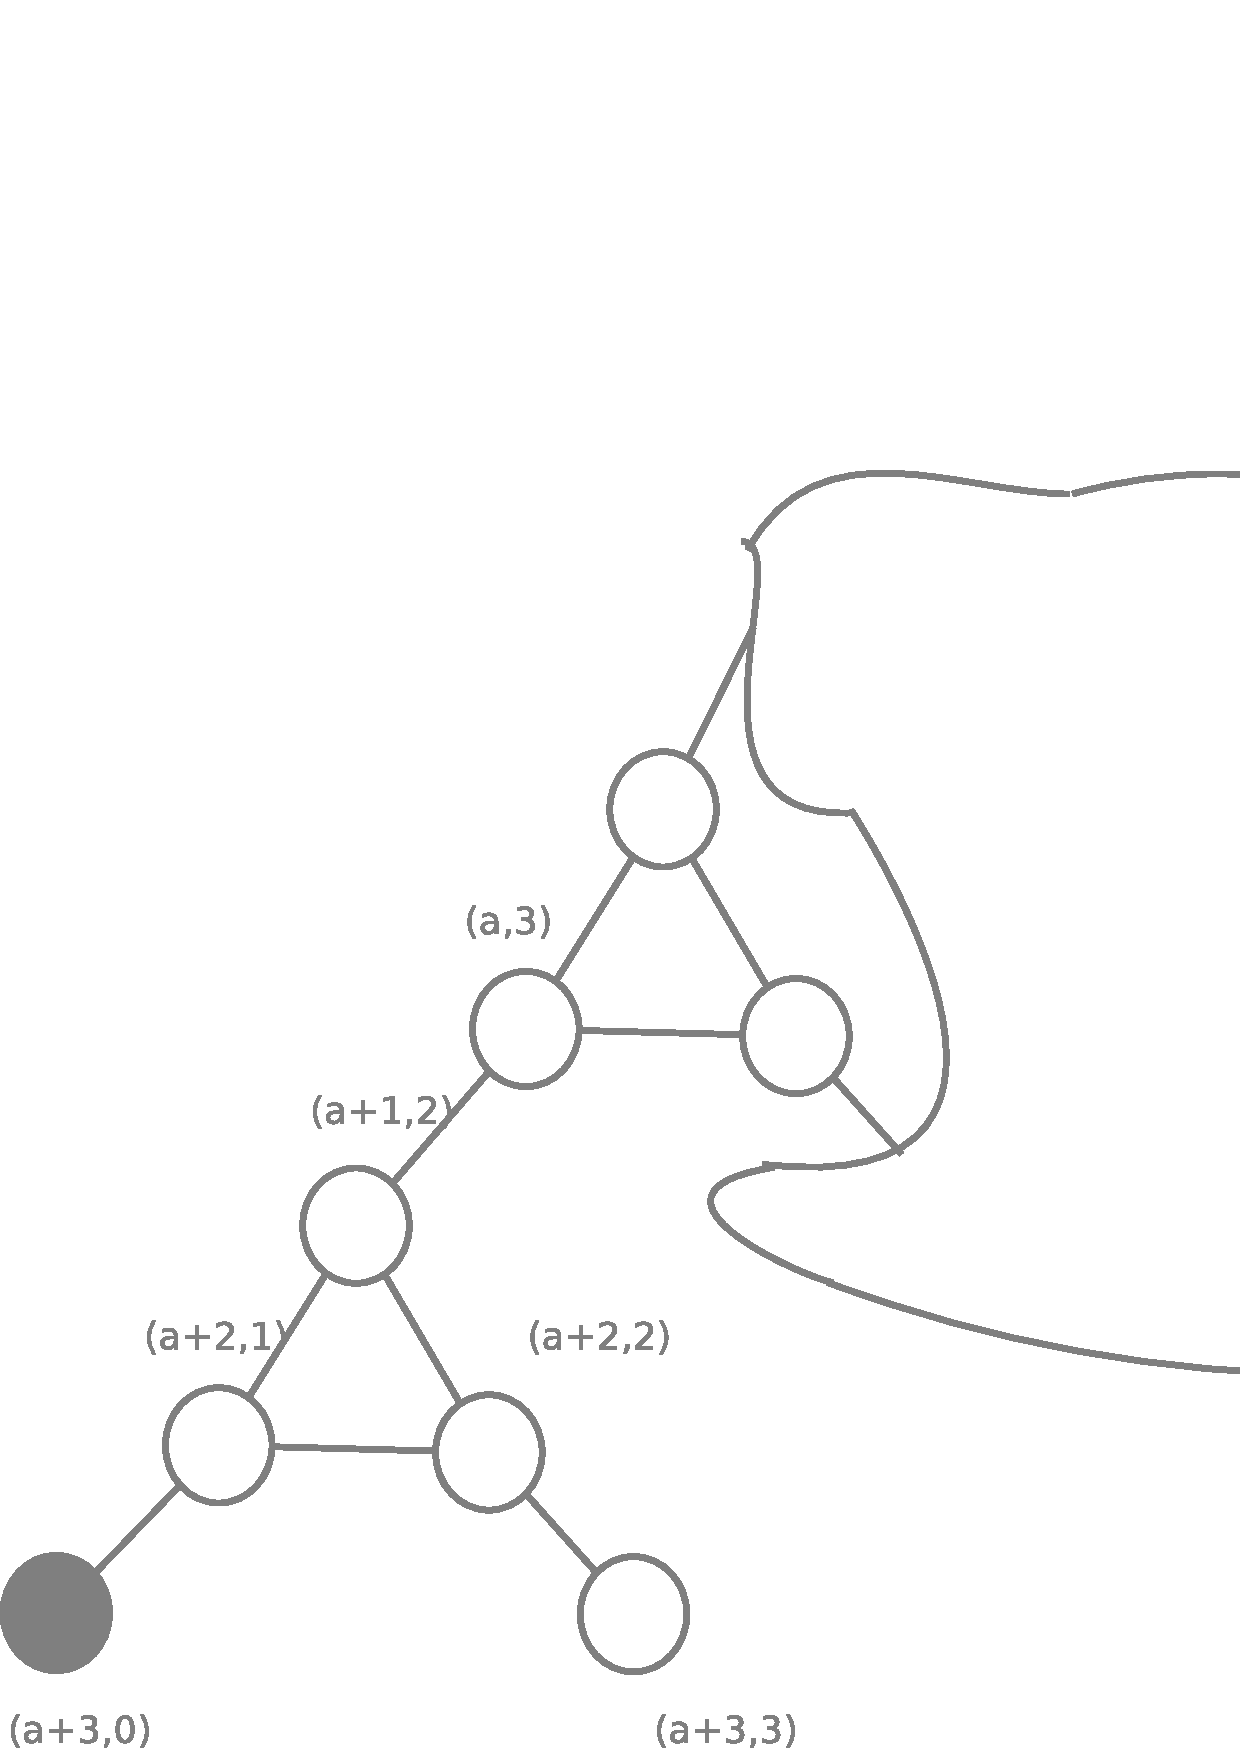
\includegraphics[width=50pt]{bilder/fall1.pdf}&\\
\hline\hline
\vspace{0.3mm}
2. Fall&\multirow{3}{121mm}{$2$ antipodale Knoten ohne Strahlen, $2$ Knoten mit/ohne Strahlen und $\frac{n}{2}-3$ Knoten ohne Strahlen der Länge $2$}\\
\cline{1-1}
\vspace{-6mm}&\\
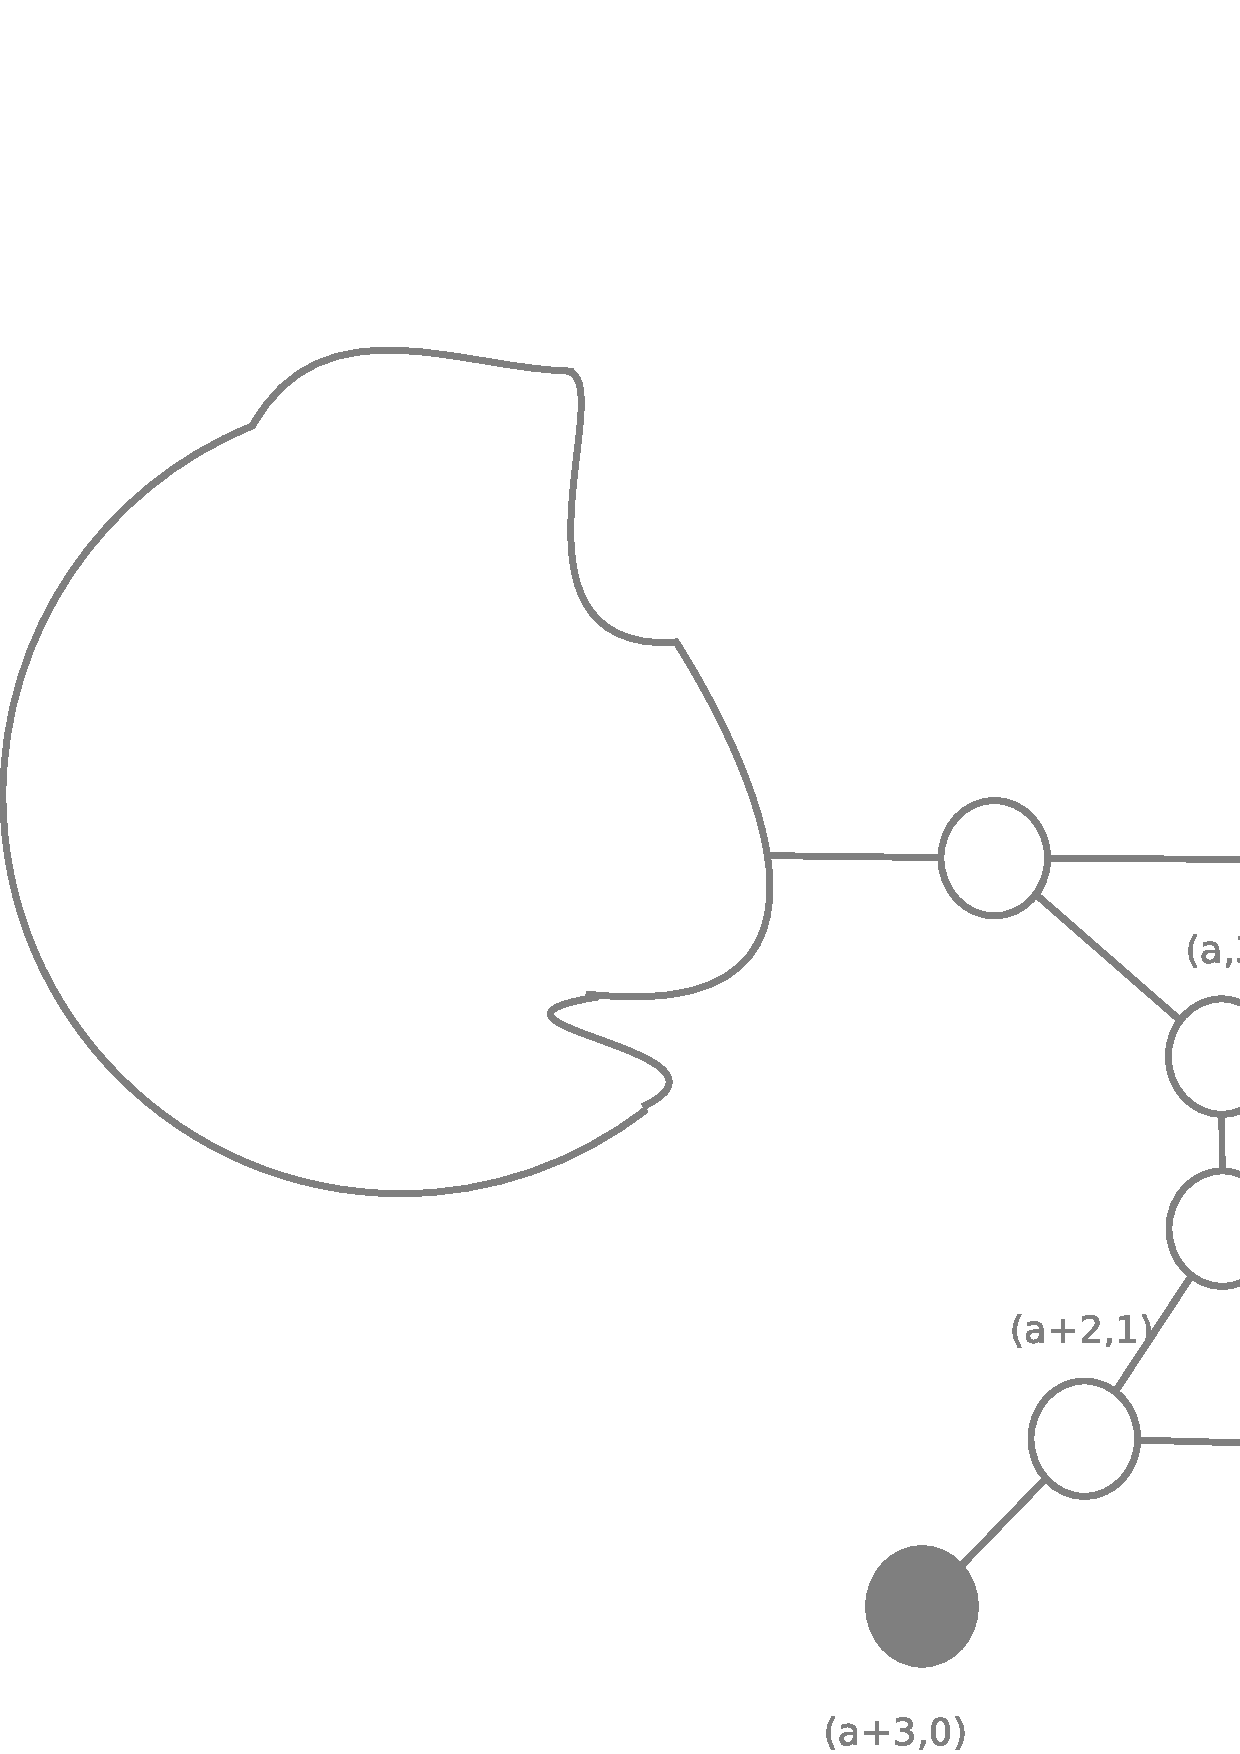
\includegraphics[width=50pt]{bilder/fall2.pdf}&\\
\hline\hline
\vspace{0.3mm}
3. Fall&\multirow{3}{121mm}{ $4$ antipodale Knoten ohne Strahlen (je $2$), $2$ Knoten mit/ohne Strahlen und $\frac{n}{2}-4$ Knoten ohne Strahlen der Länge $3$}\\
\cline{1-1}
\vspace{-6mm}&\\
\includegraphics[width=50pt]{bilder/fall3.pdf}&\\
\hline\hline
$\cdot$ &  $\cdot$\\
$\cdot$ &  $\cdot$\\
$\cdot$ &  $\cdot$\\
\hline\hline
\vspace{0.3mm}
$\frac{n}{2}-2$. Fall&\multirow{3}{121mm}{$n-2$ antipodale Knoten ohne Strahlen (je $\frac{n}{2}-1$), $2$ Knoten mit/ohne Strahlen und $1$ Knoten ohne Strahlen der Länge $\frac{n}{2}-1$}\\
\cline{1-1}
\vspace{-6mm}&\\
\includegraphics[width=50pt]{bilder/fall4.pdf}&\\
\hline\hline
\vspace{0.3mm}
$\frac{n}{2}-1$. Fall&\multirow{3}{121mm}{$n-4$ antipodale Knoten ohne Strahlen (je $\frac{n}{2}-2$)}\\
\cline{1-1}
\vspace{-6mm}&\\
\includegraphics[width=50pt]{bilder/falln2-1.pdf}&\\
\hline\hline
\end{tabularx}
\caption{Halbsonnen mit metrischer Dimension zwei}
\label{fallunterscheidungungeradesonnen2md}
\end{table}
%%%%%%%%%%%%%%%%%%%%%%%%%%%%%%%%%%%%%%%%%%%%%%%%%%%%%%%%%%%%%%%%%%%%%%%%%%%%%%%%%%%%%%%%%%%%%%%%%%%%%%%%%%%%%%%%%%%%%%%%%%%%%%%%
\newpage
\section{Vollständigen Graphen mit Strahlen $K^s_{n,i}$}

\section{Der erweiterte Gittergraph}
\subsection{Der Gittergraph mit Strahlen}
\subsection{Der Gittergraph mit Strahlen an jedem Knoten}
\section{Eine Erweiterung der Radgraphen $W_{n,i}$}
%%%%%%%%%%%%%%%%%%%%%%%%%%%%%%%%%%%%%%%%%%%%%%%%%%%%%%%%%%%%%%%%%%%%%%%%%%%%%%%%%%%%%%%%%%%%%%%%%%%%%%%%%%%%%%%%%%%%%%%%%%%%%%%%
\vspace{-2mm}
\chapter{Metrische Dimension von Kaktusgraphen}
\label{kapkaktus}
\begin{defi}
Als Kaktusgraph wird ein Graph bezeichnet, wenn alle seine Kreise paarweise kantendisjunkt sind, sich also höchstens einen gemeinsamen Knoten teilen.
\end{defi}
Ein Graph mit höchstens einem Kreis gehört zu der Graphklasse der Kaktusgraphen.\newline Einige Beispiele von Kaktusgraphen sind Wege, Bäume, Kreise, Sterne, Sonnengraphen und die $C_j-Bäume$ aus dem Kapitel \ref{kapcjbaume}.\newline Außerdem ist jeder Kaktusgraph außenplanar. Für die außenplanaren Graphen existiert ein polynomialzeit Algorithmus zur Berechnung der metrischen Dimension, welcher in dem Kapitel \ref{aussenpalanar} erläutert wird. Durch die spezifische Struktur von Kaktuspraphen lässt sich die metrische Dimension sogar in Linearzeit berechnen. Um diesen Algorithmus und die Analyse seiner Laufzeit geht es in diesem Abschnitt.
\begin{figure}[h!]
		\centering
 		 \includegraphics[width=420pt]{bilder/kaktusallg.pdf}
   \caption{Ein Kaktusgraph $G_k$}
   \label{gk}
  	 \end{figure}
  	 \vspace{-2mm}
\begin{algorithm}
\caption{Aufbau vom Algorithmus zur Berechnung der MD von Kaktusgraphen}
\begin{algorithmic}
\vspace{2mm}
\REQUIRE{Ein ungerichteter Kaktusgraph $G$}
\vspace{2mm}
\ENSURE{Die metrische Dimension $\beta(G) \in \mathbb{N^+}$}
\vspace{2mm}
\STATE 1. Bestimmung alle zweifachen Zusammenhangskomponente mit mindestens 3 Kanten\\$\;\;\;\;$und Einordnung von jedem Knoten zu einer der drei Klassen $\{0,i,A\}$ mit $i \geq 1$\\
\vspace{2mm}
\STATE 2. Erkennen von Amalgamationsknoten\\
\vspace{2mm}
\STATE 3. Berechnung der metrischen Dimension der zweifachen Zusammenhangskomponenten,\\$\;\;\;\;$Ersetzung dieser durch Bäume und Überprüfung der Amalgamationsknoten\\
\vspace{2mm}
\STATE 4. Berechnung der zusätlichen metrischen Dimension von Amalgamationsnoten\\
\vspace{2mm}
\STATE 5. Berechnung der metrischen Dimension vom Baum
\vspace{2mm}
\end{algorithmic}
\end{algorithm}
\newpage
\section{Der Algorithmus zur Berechnung der metrischen Dimension von Kakturgraphen}
\textbf{Idee:} Ein Kaktusgraph wird in einen Baum mit gleicher metrischer Dimension umgewandelt, welche dann mit einem bekannten linearzeit Algorithmus bestimmt wird.\newline\newline
Zunächst wird der gegebene Kaktusgraph in fünf unterschiedliche Komponenten partitioniert, welche durch genau einen Knoten verbunden sind. Diese Komponenten sind Kreise, Sonnen, unvollständige Sonnen, Bäume und einige besondere Wege.\newline\newline
Die unterschiedlichen Arten von Wegen sind:
\begin{itemize}
\item Wege zwischen zweifachen Zusammenhangskomponenten
\item Wege an zweifachen Zusammenhangskomponenten
\begin{itemize}
\item an einem Knoten ist nur ein Weg
\item an einem Knoten ein Weg und noch etwas Anderes (kein Baum)
\end{itemize}
\end{itemize}
Die Wege zwischen zweifachen Zusammenhangskomponenten dürfen nach Lemma \ref{first_theorem} ignoriert werden. Die induzierten Wege an zweifachen Zusammenhangskomponenten bilden mit der zweifachen Zusammenhangskomponente die Sonnen und unvollständigen Sonnen. Der letzte Fall von Wegen wird gesondert in dem Abschnitt zu Amalgamationsknoten untersucht.\newline\newline
Die zweifachen Zusammenhangskomponenten sind Kreise, Sonnen und unvollständige Sonnen. Diese werden in Schritt 4 einzeln betrachtet, dabei werden Knoten welche diese Komponenten mit anderen Teilgraphen verbinden als $A$ Knoten markiert, sofern sich in dem Teilgraphen ein Ankerknoten befindet. Die metrische Dimension wird für jeden Kreis, jede Sonne und jede unvollständige Sonne bestimmt, mit der Vorraussetzung, dass jeder $A$ Knoten ein Ankerknoten ist.\newline
Ist die metrische Dimension einer Komponente größer als die Anzahl der $A$ Knoten so wird die Komponente durch einen Baum ersetzt mit der Differenz als metrische Dimension.\newline\newline
Dadurch ist eine Trennung der Knoten in den Komponenten möglich. Um die Trennung im gesamten Graphen zu erreichen, wird für jeden Knoten der mehrere Komponenten überprüft ob nicht getrennte Knotenpaare existieren und die Anzahl der zusätzlich benötigten Ankerknoten um diese zu Trennen ermittelt. Die Anzahl dieser Ankerknoten bestimmt die letzte Veränderung des Baums. Damit ist die Transformation abgeschlossen und die metrische Dimension kann bestimmt werden.
\begin{bsp}~\newline
An dem Kaktusgraphen $G_k$ aus der Abbildung \ref{gk} wird die Funktionsweise vom Algorithmus gezeigt.
In der Abbildung \ref{kaktus1} wurden die Algorithmen \ref{alg2zssuche1} und \ref{alg2zssuche2} ausgeführt und die zweifachen Zusammenhangskomponenten $\{1, \ldots, 7\}$ von dem Kaktusgraphen $G_k$ wurden in einer Liste von Listen gespeichert. Außerdem wurden die Algorithmen \ref{algtiefen1} und \ref{algtiefen2} ausgeführt und jeder Knoten wurde einer der Klassen $\{0,i,A\}$ mit $i \geq 1$ zugewiesen. Übersichtshalber wurde die Markierung $0$ in der Abbildung \ref{kaktus1} ausgelassen.
 	   	 \begin{figure}[h!]
		\centering
 		 \includegraphics[width=350pt]{bilder/kaktusallgschritt2.pdf}
   \caption{Die zweifachen Zusammenhangskomponenten wurden bestimmt und die Knoten wurden in drei Klassen partitioniert}
      \label{kaktus1}
  	 \end{figure}
  	 ~\linebreak
  	 
  	 In der Abbildung \ref{kaktus1.2} wurde der Algorithmus \ref{algeinteilung} ausgeführt. Jede zweifache Zusammenhangskomponente wurde einzeln betrachtet und eindeutig als einer der drei Typen erkannt.
 	   	 \begin{figure}[h!]
		\centering
 		 \includegraphics[width=310pt]{bilder/kaktusallgschritt3,2.pdf}
   \caption{Die zweifachen Zusammenhangskomponenten wurden in drei Klassen partitioniert}
      \label{kaktus1.2}
  	 \end{figure}
  	 ~\linebreak
 In der Abbildung \ref{kaktus2} wurden an den Knoten der Klasse $A$ mit den Algorithmen \ref{algtiefensuchefuermindeinblatt} und \ref{algtiefensuchefuermindeinblatt2} markiert, ob es einen einfachen Weg von dem Knoten gibt. Und mit dem Algorithmus \ref{alganweisung} wurde die zusätzliche metrische Dimension der zweifachen Zusammenhangskomponenten berechnet. Außerdem wurde mittels dem Algorithmus \ref{algsonderfall1} die Amalgamationsknoten markiert.
  	   	  	   	 \begin{figure}[h!]
		\centering
 		 \includegraphics[width=350pt]{bilder/kaktusallgschritt8.pdf}
   \caption{Amalgamationsknoten wurden markiert und MD von den zweifachen Zusammenhangskomponenten ausgerechnet}
\label{kaktus2}  	
  	 \end{figure}
  	 \newpage
  	 In der Abbildung \ref{kaktus4} wurden die zweifachen Zusammenhangskomponenten durch Bäume mit der gleichen metrischen Dimension ersetzt mit dem Algorithmus \ref{algreplace} und die Amalgamationsknoten überprüft, so dass nur noch Amalgamationsknoten mit mindestens zwei ungetrennten Nachbaren in der Menge sind. Der Algorithmus \ref{algsonderfall2} bestimmt die minimale Anzahl an Knoten, welche noch aufgenommen werden müssen. In diesem Beispiel gibt es zwei Amalgamationsknoten mit jeweils zwei ungetrennten Komponenten. Beide beinhalten eine gemeinsame Komponente, dadurch reicht ein zusätzliches Element in der metrischen Basis aus um beide Nachbarschaften der Amalgamationsknoten zu trennen.
\vspace{-1mm}
  	   	 \begin{figure}[h!]
		\centering
 		 \includegraphics[width=315pt]{bilder/kaktusallgschritt10.pdf}
   \caption{Zweifache Zusammenhangskomponenten wurden ersetzt und die ungetrennten Amalgamationsknoten markiert}
   \label{kaktus4}
  	 \end{figure}
  	 \vspace{-3mm}
  	 ~\linebreak
  	 In der Abbildung \ref{kaktus6} wird ein Knoten an den zuletztbetrachteten Amalgamationsknoten hinzugefügt, da es einen einfachen Weg an dem Knoten gibt. In so einem Fall reicht ein zusätzlicher Knoten aus um die metrische Dimension des Graphen um eins zu erhöhen.
\vspace{-1mm}
  	   	 \begin{figure}[h!]
		\centering
 		 \includegraphics[width=330pt]{bilder/kaktusallgschritt12.pdf}
   \caption{Resultierender Baum mit markierter metrischer Basis}
   \label{kaktus6}
  	 \end{figure}
  	 \vspace{-3mm}
  	 ~\linebreak 
  	 In der Abbildung \ref{kaktus7} wird zum Vergleich eine metrische Basis von dem ursprünglichen Kaktusgraphen dargestellt. Ohne den Knoten $r_9$ wären die zwei hell- und dunkelroten Knotenpaare nicht getrennt.
  	 \vspace{-1mm}
  	 \begin{figure}[h!]
		\centering
 		 \includegraphics[width=310pt]{bilder/kaktusallgschritt13.pdf}
   \caption{Der ursprüngliche Kaktusgraph mit markierter metrischer Basis}
   \label{kaktus7}
  	 \end{figure}
  	 \end{bsp}
  	 \clearpage
\section{Die Laufzeitanalyse}
~\linebreak
Um zu zeigen, dass die metrische Dimension von Kaktusgraphen in Linearzeit bestimmt werden kann wurde ein Algorithmus in Pseudocode geschrieben. In diesem Abschnitt wird seine Laufzeit analysiert. Der Algorithmus selbst befindet sich im Anhang \ref{app} der Arbeit. Es wird eine Übersicht über die einzelnen Algorithmen, eine kurze Beschreibung und eine obere Schranke für ihre Laufzeit in den Tabellen \ref{übersicht1} und \ref{übersicht} angegeben.\newline
\vspace{-1mm}
\begin{table}[htp]
\centering
 \renewcommand{\arraystretch}{2}
\begin{tabularx}{\textwidth}{@{\extracolsep{\fill}}|c|c|c|}
\hline
\textbf{Algorithmus}&\textbf{Bedeutung}&\textbf{Laufzeit}\\
\hline
\vspace{-1mm}
\multirow{2}{26mm}{Algorithmus \ref{alg2zssuche1} und Algorithmus \ref{alg2zssuche2}}& Zweifache Zusammenhangskomponenten&\multirow{2}{*}{$\mathcal{O}(|V|+|E|)$}\\
\vspace{-1mm}
&mit mindestens drei Kanten werden erkannt&\\
\hline
\vspace{-1mm}
\multirow{2}{25mm}{Algorithmus \ref{algzweifachzus}}& Alle Knoten aus zweifachen Zusammenhangs-&\multirow{2}{22mm}{$\mathcal{O}(|V|+|E|)$}\\&komponenten bekommen eine Markierung&\\ 
\hline
\vspace{-1mm}
\multirow{2}{25mm}{Algorithmus \ref{algtiefen1} und Algorithmus \ref{algtiefen2}}& Die modifizierte Tiefensuche partitioniert&\multirow{2}{22mm}{$\mathcal{O}(|V|)$}\\& alle Knoten in drei Klassen&\\
\hline
\multirow{3}{25mm}{Algorithmus \ref{algeinteilung}}& Die zweifachen Zusammenhangskomponenten&  \multirow{3}{22mm}{$\mathcal{O}(|V|+|E|)$}\\& werden in Kreise, Sonnen und unvollständige&\\& Sonnen partitioniert &\\
\hline
\multirow{4}{27mm}{Algorithmus \ref{algtiefensuchefuermindeinblatt} und Algorithmus \ref{algtiefensuchefuermindeinblatt2}}& Die modifizierte Tiefensuche überprüft für&\multirow{4}{22mm}{$\mathcal{O}(|V|+|E|)$}\\&Knoten mit mindestens Grad vier in zweifachen& \\& Zusammenhangskomponenten ob ein induzierter&\\&Weg vorhanden ist&\\
%\hline
%Algorithmus \ref{algreplace}& Die Strukturen zum Ersetzen von Teilgraphen&\\& werden definiert & $\mathcal{O}(|V|+|E|)$\\
%\hline
%Algorithmus \ref{algberechnungkreis}& Die zusätzliche MD von Kreisen wird bestimmt & $\mathcal{O}(|E|)$\\
%\hline
%Algorithmus \ref{Bifurnachbar}& Die zusätzliche MD von Sonnen wird bestimmt & $\mathcal{O}(|E|)$\\
%\hline
%\multirow{3}{26mm}{Algorithmus \ref{algberechnungungeradesonne1} und Algorithmus \ref{algberechnunggeradesonne1} und Algorithmus \ref{algberechnungusonne2}}& Die zusätzliche MD von & \multirow{3}{25mm}{$\mathcal{O}(|V|+|E|+?+|V|+|E|)$}\\&unvollständigen Sonnen wird bestimmt&\\&&\\
%\hline
%Algorithmus \ref{algsonderfall2}& Die Problemknoten werden überprüft und&\\& ggf. mit zusätzlichen Knoten ergänzt& $\mathcal{O}(|V|+|E|)$\\
\hline
\end{tabularx}
\caption{Übersicht über die einzelnen Laufzeiten der Algorithmen zur Erkennung des Graphen}
\label{übersicht1}
\end{table}
~\linebreak
Die Laufzeiten aller in der Tabelle \ref{übersicht1} aufgelisteten Algorithmen wird in der Bemerkung \ref{alg123} erläutert.
\newpage
\begin{bem}[Laufzeit der Algorithmen zur Erkennung und Einteilung des Graphen]~
\label{alg123}
\begin{itemize}
\item Bei den Algorithmen \ref{alg2zssuche1} und \ref{alg2zssuche2} werden alle zweifachen Zusammenhangskomponenten erkannt und in einer Liste von Listen gespeichert, sofern die zweifache Zusammenhangskomponente aus mindestens drei Kanten besteht. Im Algorithmus gibt es zwei verschachtelte \textsc{for}-Schleifen, wobei die erste \textsc{for}-Schleife in Zeile 4 vom Algorithmus \ref{alg2zssuche1} über alle Knoten einmalig läuft. Bei der zweiten \textsc{for}-Schleife in Zeile 4 vom Algorithmus \ref{alg2zssuche2} werden nur Kanten an dem jeweiligen Knoten betrachtet wobei eine Kante in Zeile 6 einmalig auf den Stack gelegt und in Zeile 12 einmalig vom Stack genommen wird. Die asymptotische Laufzeit ist damit $\mathcal{O}(|V|+|E|)$. 
\item Der Algorithmus \ref{algzweifachzus} entscheidet ob ein Knoten in einer zweifachen Zusammenhangskomponente ist. Zunächst läuft man über alle Knoten $v$ und setzt $ZK(v)=0$. Die asymptotische Laufzeit dafür ist in $\mathcal{O}(|V|)$. Dannach werden zwei verschachtelte \textsc{for}-Schleifen benötigt. Die erste \textsc{for}-Schleife in Zeile 1 vom Algorithmus läuft über alle Zusammenhangskomponenten. Die zweite \textsc{for}-Schleife in Zeile 2 läuft über jede Kante einer zweifachen Zusammenhangskomponente. Dabei werden die inzidenten Knoten markiert. Nach der Definition eines Kaktusgraphen darf keine Kante in zwei Kreisen und somit in zwei zweifachen Zusammenhangskomponenten liegen. Der Algorithmus läuft über eine Teilmenge der Kanten einmalig drüber und hat eine  
asymptotische Laufzeit von $\mathcal{O}(|V|+|E|)$.
\item Die Algorithmen \ref{algtiefen1} und \ref{algtiefen2} sind für die Einteilung aller Knoten in Klassen zuständig. Es gibt im Algorithmus \ref{algtiefen1} in Zeile 2 eine \textsc{for}-Schleife über die Anzahl der Knoten vom Grad drei und in Zeile 4 wird der Algorithmus \ref{algtiefen2} aufgerufen, welcher eine \textsc{for}-Schleife in Zeile 2 besitzt über die Anzahl der Kanten an dem jeweiligen Knoten. Insgesamt läuft der Algorithmus für jeden Knoten über jeweils drei Kanten, also asymptotisch $\mathcal{O}(|V|+|E|)$ Schritte. Weiterhin gibt es in Zeile 7 im Algorithmus \ref{algtiefen1} eine \textsc{for}-Schleife über die Anzahl aller Knoten, damit ist die asymptotische Laufzeit in $\mathcal{O}(|V|+|E|+|V|)=\mathcal{O}(|V|+|E|)$.
\item Der Algorithmus \ref{algeinteilung} ändert die Darstellung der zweifachen Zusammenhangskomponenten von Kanten auf Knoten. Dafür gibt es die \textsc{for}-Schleife in Zeile 2 über alle zweifachen Zusammenhangskomponente und die \textsc{for}-Schleife in Zeile 4 über jeweils die Kanten in einer zweifachen Zusammenhangskomponente. Die  asymptotische Laufzeit in $\mathcal{O}(|E|)$, da jede Kante in maximal einer Zusammenhangskomponente liegt. In den Zeilen 18 und 19 sind zwei \textsc{for}-Schleifen, die erste \textsc{for}-Schleife läuft über alle zweifachen Zusammenhangskomponenten und die zweite \textsc{for}-Schleife über alle Knoten in einer zweifachen Zusammenhangskomponente. Ein Knoten kann in beliebig vielen zweifachen Zusammenhangskomponenten sein, aber eine Kante nur in maximal einer. Damit läuft dieser Teil vom Algorithmus über jede Kante maximal zwei mal und ist in $\mathcal{O}(2 \cdot |E|)=\mathcal{O}(|E|)$.
\item Die Algorithmen \ref{algtiefensuchefuermindeinblatt} und \ref{algtiefensuchefuermindeinblatt2} überprüfen für Knoten der Klasse $A$ ob ein Blatt über Knoten vom Grad zwei erreicht wird. Dafür wird in Algorithmus \ref{algtiefensuchefuermindeinblatt} in Zeile 1 eine \textsc{for}-Schleife, welche über alle Knoten läuft, benötigt.
Im Algorithmus \ref{algtiefensuchefuermindeinblatt2} gibt es eine weitere \textsc{for}-Schleife über die Kanten des jeweiligen Knotens. Die asymptotische Laufzeit ist in $\mathcal{O}(|V|+|E|)$.
\end{itemize}
\end{bem}
\newpage
\begin{table}[htp]
\centering
 \renewcommand{\arraystretch}{2}
\begin{tabularx}{\textwidth}{@{\extracolsep{\fill}}|c|c|c|}
\hline
\textbf{Algorithmus}&\textbf{Bedeutung}&\textbf{Laufzeit}\\
\hline
Algorithmus \ref{algsonderfall1}& Amalgamationsnoten werden markiert & $\mathcal{O}(|V|+|E|)$\\
\hline
\multirow{2}{*}{Algorithmus \ref{algreplace}}& Die Strukturen zum Ersetzen von Teilgraphen&\multirow{2}{*}{$\mathcal{O}(|V|+|E|)$}\\& werden definiert & \\
\hline
Algorithmus \ref{alganweisung}& Die Klasse einer ZK wird erkannt & $\mathcal{O}(|E|)$\\
\hline
Algorithmus \ref{algberechnungkreis}& Die zusätzliche MD von Kreisen wird bestimmt & $\mathcal{O}(|E|)$\\
\hline
Algorithmus \ref{algberechnungsonne}& Die zusätzliche MD von Sonnen wird bestimmt & $\mathcal{O}(|E|)$\\
\hline
\multirow{3}{26mm}{Algorithmus \ref{algberechnungungeradesonne1} und Algorithmus \ref{algberechnunggeradesonne1} und Algorithmus \ref{algberechnungusonne2}}& Die zusätzliche MD von & \multirow{3}{25mm}{$\mathcal{O}(|V|+|E|)$}\\&unvollständigen Sonnen wird bestimmt&\\&&\\
\hline
\multirow{2}{*}{Algorithmus \ref{algsonderfall2}}& Die Amalgamationsknoten werden überprüft und& \multirow{2}{*}{$\mathcal{O}(|V|+|E|)$}\\& ggf. mit zusätzlichen Knoten ergänzt&\\
\hline
\end{tabularx}
\caption{Übersicht über die einzelnen Laufzeiten der Algorithmen zur Berechnung der metrischen Dimension einzelner Komponenten}
\label{übersicht}
\end{table}
\begin{bem}~
\begin{itemize}
\item Der Algorithmus \ref{algsonderfall1} läuft einmal am Anfang über jede Kante in jeder zweifachen Zusammenhangskomponente und speichert dabei den Abstand zwischen zwei Ankerknoten. An jedem Knoten wird nebenbei der größere von den beiden Abständen zu dem nächsten Ankerknoten gespeichert und an jeder zweifachen Zusammenhangskomponente der größte Abstand zwischen zwei Ankerknoten in dieser Komponente. Geschickt kann man alle diese Werte erfahren in dem man zwei mal über den Graphen läuft und sich an jedem Knoten den linken und rechten Nachbar speichert. Damit ist man asymptotisch in $\mathcal{O}(|V|+|E|)$.

\item Der Algorithmus \ref{alganweisung} überprüft für jede zweifache Zusammenhangskomponente welcher Klasse sie angehört und ruft einen eintsprechenden Algorithmus zur Berechnung der Komponente auf. Es gibt eine \textsc{for}-Schleife in Zeile 1 über alle zweifache Zusammenhangskomponenten, von welchen es höchstens $\frac{|E|}{3}$ gibt. Die asymptotische Laufzeit ist in $\mathcal{O}(|E|)$.

\item In dem Algorithmus \ref{algreplace} werden für eine zweifache Zusammenhangskomponente alle Knoten mit der Markierung $i$ für $i \geq 0$ mit ggf. den zugehörigen Wegen entfernt. Dieser Algorithmus wird für jede zweifache Zusammenhangskomponente genau einmal aufgerufen und liegt selbst asymptotisch in $\mathcal{O}(|V|+|E|)$.
Das Einfügen von einem neuen Knoten liegt in $\mathcal{O}(1)$, genauso wie das Einfügen von einer konstanten Anzahl von Kanten oder Knoten. Das Verbinden von einem Knoten mit allen $A$ Knoten in einer zweifachen Zusammenhangskomponente liegt in $\mathcal{O}(|V|)$ für alle zweifachen Zusammenhangskomponenten.

\item Die Algorithmen \ref{algberechnungkreis} und \ref{algberechnungsonne} berechnen die zusätliche Anzahl der Knoten in der metrische Basis für den Fall dass eine zweifache Zusammenhangskomponente eine Sonne oder ein Kreis ist. Beide Algorithmen bestehen ausschließlich aus \textsc{if}-Abfragen, die in konstanter Zeit durchgeführt werden können. Die Algorithmen rufen den Algorithmus \ref{algreplace} einmalig auf. Dieser benötigt $\mathcal{O}(|V|+|E|)$.

\item Die Algorithmen \ref{algberechnungungeradesonne1}, \ref{algberechnunggeradesonne1} und \ref{algberechnungusonne2} berechnen die zusätzliche metrische Dimension von unvollständigen Sonnen. Der Algorithmus \ref{algberechnungungeradesonne1} überprüft die ''einfachen'' Fälle, dabei wird eine zusätzliche \textsc{for}-Schleife benötigt, für den Fall, dass zwei Ankerknoten vorhanden sind und diese eine Sonne nicht trennen würden. Dafür wird mittels Tiefensuche einmalig die zweifache Zusammenhangskomponente überprüft ob bestimmte Knoten der Klasse $0$ angehören. Weiterhin wird der Algorithmus \ref{algreplace} aufgerufen, welcher asymptotisch in $\mathcal{O}(|V|+|E|)$ liegt.\\
Der Algorithmus \ref{algberechnungusonne2} betrachtet unvollständige Sonnen sofern mindestens drei und höchstens $\frac{n}{2}$ Ankerknoten vorhanden sind. Wäre eine Sonne durch die vorhandenen Ankerknoten nicht getrennt, müssen bestimmte Knoten in der zweifachen Zusammenhangskomponente überprüft werden. Dies kann mittels Tiefensuche geschehen und es wird ein asymptotischer Aufwand von $\mathcal{O}(|V|+|E|)$ benötigt.\\
Der Algorithmus \ref{algberechnunggeradesonne1} läuft über die zweifache Zusammenhangskomponente in Zeile 2,6,20 und 24. Bei der Anweisung in Zeile 2 und Zeile 20 läuft man mittels Tiefensuche über die zweifache Zusammenhangskomponente und arbeitet mit einem Zähler, der die Anzahl von aufeinanderfolgenden Knoten der Klasse $0$ zählt. Bei den Anweisungen in Zeile 6 und Zeile 24 wird zusätzlich bei jedem Schritt die Klasse von dem gegenüberliegendem Knoten überprüft. Da die Knoten eine Nummerierung haben kann man auf den $i$-ten und den $i+\frac{n}{2}$-ten Knoten direkt zugreifen und die Klasse überprüfen. Die einzelnen zusammenhängenden Mengen von Knoten der Klasse $0$ werden mit ihren gegenüberliegenden Knoten in einer Liste von Listen gespeichert. Jeder Knoten kommt maximal in einer Liste vor, denn jeder Knoten gehört zu genau einer zusammenhängenden Menge der Klasse $0$.
\item Der Algorithmus \ref{algsonderfall2} berechnet für einen Amalgamationsknoten die Anzahl der zusätzlichen Knoten für die Aufnahme in die metrische Basis um seine Nachbarschaft zu trennen. Dafür werden die zweifachen Zusammenhangskomponenten welche inzident sind mit einem Knoten untersucht und ggf. mit einer Baumstruktur ergänzt. Dieser zusätzlich eingefügte Teilgraph stellt sicher, dass die metrische Dimension von dem Kaktusgraphen gleich der metrischen Dimension vom Baum ist.\\
In den Zeilen 1 und 2 gibt es zwei \textsc{for}-Schleifen für jeden Knoten über die zugehörige Menge von zweifachen Zusammenhangskomponenten iterieren. Jede Kante ist in genau einer Zusammenhangskomponente. Durch die Endknoten dieser Kante kann die Zusammenhangskomponente für diese Kante zu zwei Knoten zugeordnet werden. Jeder Knoten hat genau zwei inzidente Kanten in der gleichen Zusammenhangskomponente. An jedem Knoten gibt maximal einen Weg, der zusätzlich als Komponente gezählt wird. Insgesamt ist die Laufzeit für diese zwei \textsc{for}-Schleifen asymptotisch in $\mathcal{O}(|V|+|E|)$. Weiterhin gibt es noch eine weitere \textsc{for}-Schleife in Zeile 14, wenn bei einigen Amalgamationsknoten zusätzliche Knoten eingefügt werden. Die Anzahl der Knoten ist beschränkt durch die Anzahl der Komponenten welche inzident sind zu dem Knoten. Aufgrund des gleichen Arguments ist die Laufzeit in $\mathcal{O}(|V|+|E|)$ und damit insgesamt aus $\mathcal{O}(|V|+|E|+|V|+|E|)=\mathcal{O}(|V|+|E|)$.
\end{itemize}
\end{bem}
\section{Der Korrektheitsbeweis vom Algorithmus}
Zu zeigen ist, dass die Idee den Algorithmus in angegeben Teile zu partitionieren richtig ist, dass die Partitionierung richtig gemacht wird. Außerdem dass alle Fälle für die Berechnung komplett sind und dass alle Fälle bei der Berechnung abgedeckt werden. Außerdem dass der Austausch der Komponente in Baumkomponenten ohne Nebenwirkung abläuft.\newline\newline
Einer der Gründe weshalb es keinen einfachen und effizienten Algorithmen für die Berechnung der metrischen Dimension gibt, ist dass sich das Problem nicht lokal auf Teilgraphen lösen lässt und die metrische Dimension für den Gesamtgraphen nicht einfach die Summe der Komponenten ist (vgl. Kapitel \ref{kapallg}).\newline\newline
Die Kaktusgraphen haben durch die starken Einschränkungen der Struktur nur ''eine handvoll'' unterschiedlicher Komponenten als Bestandteile, welche durch jeweils einen Trennungsknoten verbunden sind. Dazu gehören Bäume, Wege und Kreise.\newline\newline
Nach dem Lemma \ref{wegtrennungsknoten} kann ein Trennungsknoten lokal als Ankerknoten aufgefasst werden. Hierbei bedeutet lokal, dass man nur einen Teilgraph mit dem Trennungsknoten als Gesamtgraph betrachtet. Aus dem Lemma \ref{einelementreichtnicht} ist bekannt, dass ein Teilgraph, welcher kein Kreis ist immer mindestens einen Ankerknoten beinhaltet. Daraus folgt aber nicht, dass Wege keine Ankerknoten haben können. Es bedarf einer gesonderten Untersuchung wie sich Wege als Teilgraphen verhalten. Ein Weg kann an einem Baum vorkommen, es bleibt aber für die Untersuchung ein Baum. Außerdem kann ein Weg an einem Kreis vorkommen. Es entsteht dadurch eine voll- oder unvollständige Sonne. Der Fall, dass mehrere Kreise und ein Weg an einem Knoten vorkommen wird ebenfalls untersucht. Weitere Möglichkeiten gibt es nicht. \newline
Der Abschnitt \ref{korraufteilung} zeigt, dass der Algorithmus im Anhang die Bestandteile des Graphens richtig erkennt und aufteilt. Der Abschnitt \ref{korrkomp} behandelt die Korrektheit der Berechnung der metrischen Dimension einzelner Komponenten.\newline\newline
Eine Sache muss bei der Berechnung des Gesamtgraphen gegenüber der Berechnung der einzelner Komponenten beachtet werden. Nach dem Lemma \ref{trennungsknoten} sind alle Knotenpaare getrennt, welche sich in zwei Teilgraphen mit jeweils mindestens einem Ankerknoten befinden und mit mindestens einer Kante verbunden sind. Damit vereinfacht sich die Betrachtung auf einen einzigen Fall, und zwar wenn zwei oder mehr Teilgraphen mit einem Trennungsknoten direkt verbunden sind. Der Trennungsknoten muss dafür mindestens der Grad vier haben. Um die korrekte Erkennung und Berechnung dieses Falles geht es in dem Abschnitt \ref{korramal}.\newline\newline
Die letzte Frage die geklärt werden muss, ist warum man bei Kaktusgraphen die Komponenten einzeln betrachten darf. Wären alle Komponenten mit jeweils mindestens einer Kante verbunden, so würde nach dem Lemma \ref{trennungsknoten} durch eine Trennung der Komponenten direkt eine Trennung des Gesamtgraphen folgen. Diese Eigenschaft kann aber nur für Komponenten benutzt werden welche mit mindestens einer Kante verbunden sind. Für die anderen Kompositionen gilt nach Lemma \ref{nachbartrennungsknoten}, dass wenn alle Nachbarn eines Trennungsknotens getrennt sind, sind auch alle Knotenpaare in jeweils unterschiedlichen Komponenten getrennt. In dem Abschnitt \ref{korramal} wird explizit gezeigt warum die Anzahl der zusätzlich gewählten Ankerknoten minimal ist.
\subsection{Die Korrektheit der Aufteilung}
\label{korraufteilung}
Die Korrektheit der Tiefensuche, sowie die Korrektheit vom Algorithmus zur Erkennung der 2-fachen Zusammenhangskomponenten werden vorrausgesetzt.\\
Für Kaktusgraphen ist es bekannt, dass jede zweifache Zusammenhangskomponente mit mindestens drei Knoten ein Kreis ist.\cite{}. Da nach Vorraussetzung die Algorithmen \ref{alg2zssuche1} und \ref{alg2zssuche2} die zweifachen Zusammenhangskomponenten korrekt erkennen, kann der Algorithmus \ref{algzweifachzus} diese Komponenten korrekt markieren.
\begin{bem}
Ordne jeden Knoten jeder zweifachen Zusammenhangskomponente zu einer der drei Klassen $\{0,i,A\}$ mit $i \geq 1$
\begin{itemize}
\item Es gibt keine Knoten mit Grad eins auf einem Kreis.
\item Alle Knoten mit Grad zwei sind der Klasse $0$ zugeordnet.
\item Alle Knoten mit Grad $\geq 4$ sind der Klasse $A$ zugeordnet.
\item Es fehlt die Zuordnung der Knoten mit Grad $3$, dazu dienen die Algorithmen \ref{algtiefen1} und \ref{algtiefen2}.
\end{itemize}
\end{bem}
\subsection{Die Korrektheit der Berechnung der metrischen Dimension einzelner Komponenten}
\label{korrkomp}
\textbf{Kreise}\newline
Die metrische Dimension von einem Kreis ist zwei. In der Arbeit ''Resolvability and the upper dimension of graphs'' \cite{upper} behandeln Gary Chartrand, Christopher Poisson und Ping Zhang die Oberdimension von Kreisen. Die Oberdimension ist die minimale Anzahl von Knoten so dass jede Menge eine metrische Basis ist.\newline
Für Kreise mit einer ungeraden Anzahl von Knoten ist die Oberdimension zwei.\newline
Für Kreise mit einer geraden Anzahl von Knoten ist die Oberdimension drei, denn zwei gegenüberliegende Knoten können keinen Kreis trennen. Algorithmisch muss also untersucht werden, ob es mindestens zwei Knoten der Klasse $A$ gibt und falls dies nicht der Fall ist, werden maximal zwei Knoten in die metrische Basis aufgenommen. Bei einem Kreis mit einer geraden Anzahl von Knoten und genau zwei Knoten der Klasse $A$, wird überprüft ob sich die Knoten der Klasse $A$ gegenüber liegen.\newline\newline
\textbf{Sonnen}\newline
Die metrische Dimension 
\textbf{Halbsonnen}\newline
\textbf{Bäume}\newline
\textbf{Wege an Knoten der Klasse $A$}\newline
\subsection{Die Korrektheit der Erkennung und Berechnung der metrischen Dimension bei Amalgamationsknoten}
\label{korramal}
Der Graph besteht aus unterschiedlichen Komponenten, darunter sind Kreise, Sonnen, unvollständige Sonnen, Bäume und Wege zwischen Komponenten. Ein Knoten kann gleichzeitig zu mehreren Komponenten gehören, eine Kante hingegen gehört immer zu genau einer Komponente. Damit liefert die Aufteilung der Kanten in Komponenten eine Partitionierung des Graphen.\newline 
Angenommen zwei Knoten in einer Komponente haben die gleiche metrische Dimension. 
Angenommen zwei Knoten in unterschiedlichen Komponenten haben die gleiche metrische Dimension. 
\begin{comment}
\large{Induktion über die Anzahl der Komponenten $k$}\newline
\textbf{Induktionsanfang:}
\begin{itemize}
\item{Fall $k=0$:} Der Graph ist ein Weg. $\Longrightarrow$ Die metrische Dimension ist eins.
\item{Fall $k=1$:} Der Graph ist ein Baum, ein Kreis, eine Sonne oder eine unvollständige Sonne. Da es nur eine Komponente gibt, muss kein Sonderfall an den Trennungsknoten beachtet werden. 
\begin{itemize}
\item Baum\\
Die metrische Dimension kann mit dem Algorithmus von \cite{} bestimmt werden.
\item Kreis\\
Die metrische Dimension ist zwei.
\item Sonne\\
Die metrische Dimension ist für gerade Sonnen drei und für ungerade Sonnen zwei.
\item unvollständige Sonne\\
Die metrische Dimension ist für ungerade, unvollständige Sonnen zwei. Für gerade, unvollständige Sonnen wird überprüft ob einer in der Tabelle \ref{tab} aufgelisteten Fälle eintritt, dann ist die metrische Dimension zwei. Ist dies nicht der Fall so ist die metrische Dimension drei.
\end{itemize}
\item{Fall $k\to k+1$:} Angenommen, die metrische Dimension wurde für $k$ andere Komponenten korrekt berechnet. 
Wird nun die $k+1$-Komponente überprüft. Sei $l$ die Anzahl der Trennungsknoten in der Komponente $k$.
\begin{itemize}
\item Kreis 
\begin{itemize}  
\item $l\geq 3$\\
Die metrische Dimension ist $k$.
\item $l=1$\\
Die metrische Dimension ist $k+1$.
\item $lk=2$\\
Wenn $k$ ein ungerader Kreis ist  
\end{itemize}
\item Sonne\\
Die metrische Dimension ist für gerade Sonnen drei und für ungerade Sonnen zwei.
\item unvollständige Sonne\\
Die metrische Dimension ist für ungerade, unvollständige Sonnen zwei. Für gerade, unvollständige Sonnen wird überprüft ob einer in der Tabelle \ref{tab} aufgelisteten Fälle eintritt, dann ist die metrische Dimension zwei. Ist dies nicht der Fall so ist die metrische Dimension drei.
\end{itemize}
\end{itemize}
\end{comment}

%%%%%%%%%%%%%%%%%%%%%%%%%%%%%%%%%%%%%%%%%%%%%%%%%%%%%%%%%%%%%%%%%%%%%%%%%%%%%%%%%%%%%%%%%%%%%%%%%%%%%%%%%%%%%%%%%%%
Für die Berechnung der metrischen Dimension von Sonnengraphen sind unterschiedliche Fälle zu beachten:
\begin{itemize}
\item Kreis gerader oder ungerader Länge?
\item An wievielen Knoten befinden sich Wege, welche Länge haben diese und wie sind sie positioniert?
\item Gibt es bereits Teilgraphen mit Ankerknoten, wieviele gibt es und wo sind sie positioniert?
\end{itemize}
Um nicht jeden Fall einzeln zu beachten kann man mehrere Zusammenfassen, so z.B. Kreise gerader und ungerader Länge in vielen Fällen.
Für den Fall, dass es mehr als einen Ankerknoten bereits gibt reicht die Aufnahme von maximal einem weiteren Knoten in die metrische Basis aus um einen Kreis oder einen beliebigen Sonnengraphen zu trennen.
%%%%%%%%%%%%%%%%%%%%%%%%%%%%%%%%%%%%%%%%%%%%%%%%%%%%%%%%%%%%%%%%%%%%%%%%%%%%%%%%%%%%%%%%%%%%%%%%%%%%%%%%%%

Ein Knoten $u$ kann zu 
\begin{enumerate}
\item einem Weg 
\item einem Baum
\item einem Kreis
\end{enumerate}
oder beliebiger Kombinationen von diesen drei Arten gehören. Diese Kombinationen sind:\newline
~\linebreak
\begin{tabular}{lccc}
Kombination & $ZK[u]=$ & $Klasse[u]=$ & ''markiert''\\
$\cdot$ ein Weg& $0$& $0$ & ja\\
$\cdot$ ein Baum& $0$& $0/A$& nein\\
$\cdot$ ein Kreis& $1$& $0$& nein\\
$\cdot$ ein Kreis und ein Weg& $1$&$j$ mit $j\geq 1$& ja\\
$\cdot$ $i$ Kreise mit $i\geq 2$& $1$& $A$ & nein\\
$\cdot$ $i$ Kreise mit $i\geq 2$ und ein Weg &$1$& $A$& nein\\
$\cdot$ $i$ Kreise mit $i\geq 1$ und ein Baum & $1$& $A$& ja/nein\\
oder eine Verbindung zu einem anderen Kreis&&&\\
\end{tabular}
~\linebreak
Gehört ein Knoten zu mehreren Wegen, so gehört er zu einem Baum. Die Kombination aus mehreren Bäume bleibt ein Baum. Ein Baum und ein Weg werden auch zu einem Baum. Ein Kreis bleibt in beliebiger Kombination ein Kreise und so auch eine beliebige Anzahl von Kreisen.\newline\newline
Ist ein Knoten der einzige Trennungsknoten in einer zweifachen Zusammenhangskomponente so haben alle seine Nachbaren in dieser Komponente die gleiche Markierung. Um diese Knoten zu trennen müssen weitere Knoten in die metrische Basis aufgenommen werden. Die genaue Anzahl wird in Teil drei vom Algorithmus bestimmt.\\
Können Knoten aus unterschiedlichen Komponenten durch Ankerknoten aus unterschiedlichen Komponenten nicht getrennt werden?\newline
Die Antwort ist ja, aber nur bei benachbarten Komponenten, welche einen gemeinsamen Knoten teilen.
Dies gilt nicht für Zusammenhangskomponenten, die nicht unmittelbar verbunden sind. Nach Bemerkung \ref{aussagetrennungsgraphen} und dem Satz \ref{first_theorem} können keine zwei Ankerknoten aus unterschiedlichen Teilgraphen keine zwei Knoten in unterschiedlichen Teilgraphen nicht trennen, wenn da ein Weg, oder ein anderer Teilgraph zwischen liegt.\newline\newline
Zu separaten Untersuchung bleiben damit Knoten $v$ mit $Klasse[v]=A$ und mit dem $deg(v)\geq 4$. Es gibt bestimmte Kombinationen die nochmal separat untersucht werden müssen, diese sind:
\begin{enumerate}
\item $i$ Kreise mit $i\geq 2$
\item $i$ Kreise mit $i\geq 2$ und ein Weg
\item $i$ Kreise mit $i\geq 1$ und ein Baum
\end{enumerate}
\begin{tabular}{lcccc}
Kombination & $ZK[u]=$ & $Klasse[u]=$ & ''markiert''& $Weg[u]=$ \\
$\cdot$ $i$ Kreise mit $i\geq 2$& $1$& $A$ & nein& $0$\\
$\cdot$ $i$ Kreise mit $i\geq 2$ und ein Weg &$1$& $A$& nein &$1$\\
$\cdot$ $i$ Kreise mit $i\geq 1$ und ein Baum & $1$& $A$& ja/nein &$0/1$\\
\end{tabular}
%%%%%%%%%%%%%%%%%%%%%%%%%%%%%%%%%%%%%%%%%%%%%%%%%%%%%%%%%%%%%%%%%%%%%%%%%%%%%%%%%%%%%%%%%%%%%%%%%%%%%%%%%%%%%%
\begin{figure}[h!]
		\centering 		 
   \includegraphics[width=350pt]{bilder/algorithmus.pdf}
	\caption{Unterschiedliche Bäume mit denen die Komponenten ersetzt werden}
  	 \end{figure}
\newpage
%%%%%%%%%%%%%%%%%%%%%%%%%%%%%%%%%%%%%%%%%%%%%%%%%%%%%%%%%%%%%%%%%%%%%%%%%%%%%%%%%%%%%%%%%%%%%%%%%%%%%%%%%%%%%%%%
%%%%%%%%%%%%%%%%%%%%%%%%%%%%%%%%%%%%%%%%%%%%%%%%%%%%%%%%%%%%%%%%%%%%%%%%%%%%%%%%%%%%%%%%%%%%%%%%%%%%%%%%%%%%%%%%
%%%%%%%%%%%%%%%%%%%%%%%%%%%%%%%%%%%%%%%%%%%%%%%%%%%%%%%%%%%%%%%%%%%%%%%%%%%%%%%%%%%%%%%%%%%%%%%%%%%%%%%%%%%%%%%%
%%%%%%%%%%%%%%%%%%%%%%%%%%%%%%%%%%%%%%%%%%%%%%%%%%%%%%%%%%%%%%%%%%%%%%%%%%%%%%%%%%%%%%%%%%%%%%%%%%%%%%%%%%%%%%%%

%%%%%%%%%%%%%%%%%%%%%%%%%%%%%%%%%%%%%%%%%%%%%%%%%%%%%%%%%%%%%%%%%%%%%%%%%%%%%%%%%%%%%%%%%%%%%%%%%%%%%%%%%%%%%%%%
\section{Verallgemeinerungen}
Unterschiedliche Möglichkeiten sind für die Verallgemeinerung von $C_3-$Bäumen möglich. Einerseits ist es möglich die Kreisordnung zu erhöhen. Eine andere Möglichkeit ist es jeden Knoten durch einen Kreis, welcher aus sovielen Knoten besteht wie der Grad des ersetzten Knotens, zu ersetzen und jeden Knoten eindeutig einem Nachbarn zuzuordnen.

\begin{defi}
Sei ein Baum $T=(V,E)$ mit $deg(v_i)\leq j$ für $v_i \in V$ gegeben. Der $C_j-Baum$ resultiert daraus folgend: 
Für alle $3 \leq i \leq j$ und $i \in \mathbb{N}$ sei $$V'=\{v_k|v_k \in V \wedge deg(v_k)=i\}\subseteq V$$ eine Teilmenge der Knoten aus dem Graphen $T$. Ersetze jedes Knoten $v_n \in V'$ durch einen $C_k$ mit $k \geq i$ (bezeichnet wird dieser Teilgraph als \emph{$C_{k,i,n}$}), so dass höchstens ein Knoten von $C_{k,i,n}$ mit genau einem Nachbarn von $v_n$ verbunden ist. Die $i$ Nachbarn von $C_{k,i,n}$ werden als \emph{$C_{k,i}-Kinder$} bezeichnet. Sofern zwei dieser $C_{k,i}-Kinder$ Blätter sind wird der Teilgraph, welcher den $C_{k,i,n}$ und seine Nachbarn beinhaltet, als \emph{$C_{k,i}-Blatt$} bezeichnet.
\end{defi}

\begin{bsp}~\newline

\end{bsp}

\begin{bem}
Da ein $C_j$-Baum ein Kaktusgraph ist, kann die metrische Dimension von $C_j$-Bäumen mit dem Algorithmus für die Berechnung der metrischen Dimension für Kaktusgraphen bestimmt werden. Es kann auch eine vereinfachte Variante verwendet werden, die folgend aussieht:\newline
\begin{algorithm}
\caption{Aufbau vom Algorithmus zur Berechnung der MD von $C_j$-Bäumen}
\begin{algorithmic}
\vspace{2mm}
\STATE 1. Initialisiere den Graph
\vspace{2mm}
\STATE 2. Bestimme alle zweifachen Zusammenhangskomponente mit mindestens 3 Kanten\\
\vspace{2mm}
\STATE 3. Ordne jeden Knoten jeder Zusammenhangskomponente zu einer der drei Klassen\\$\;\;\;\;\{0,i,A\}$ mit $i \geq 1$\\
\vspace{2mm}
\STATE 4. Berechne die metrische Dimension der Sonnengraphen und ändere die Komponente in Bäume\\
\vspace{2mm}
\STATE 5. Berechne die metrische Dimension vom Baum
\vspace{2mm}
\end{algorithmic}
\end{algorithm}
~\linebreak
Da alle Knoten in einem $C_j$-Baum maximal den Grad drei haben tritt der Sonderfall nicht ein. Außerdem gibt es in $C_j$-Bäumen keine Kreise, sondern nur vollständige und unvollständige Sonnen.

\end{bem}
%%%%%%%%%%%%%%%%%%%%%%%%%%%%%%%%%%%%%%%%%%%%%%%%%%%%%%%%%%%%%%%%%%%%%%%%%%%%%%%%%%%%%%%%%%%%%%%%%%%%%%%%%%%%%%%%
\section{Vergleich der metrischen Dimension zwischen Bäumen und $C_j-$Baümen}
\begin{lem}
Die metrische Dimension eines $C_j$-Baumes ist immer kleiner oder gelich der metrischen Dimension des zugehörigen Baumes.
\end{lem}
Das folgende Beispiel zeigt den maximalen Unterschied der metrischen Dimension eines $C_j$-Baumes und des zugehörigen Baumes.
\begin{bsp}~\newline
\begin{figure}[ht]
\centering
\includegraphics*[width = 410pt]{bilder/bspcjbaum1.pdf}
\caption{Ein Baum mit $2nk+2$ Knoten und metrischer Dimension $2nk+2n-2k+2$}
\end{figure}
\begin{figure}[ht]
\centering
\includegraphics*[width = 410pt]{bilder/bspcjbaum2.pdf}
\caption{Der zugehörige $C_j$-Baum mit Knoten $4nk+2$ und metrischer Dimension $2$}
\end{figure}
\end{bsp}
%%%%%%%%%%%%%%%%%%%%%%%%%%%%%%%%%%%%%%%%%%%%%%%%%%%%%%%%%%%%%%%%%%%%%%%%%%%%%%%%%%%%%%%%%%%%%%%%%%%%%%%%%%%%%%%%
%%%%%%%%%%%%%%%%%%%%%%%%%%%%%%%%%%%%%%%%%%%%%%%%%%%%%%%%%%%%%%%%%%%%%%%%%%%%%%%%%%%%%%%%%%%%%%%%%%%%%%%%%%%%%%%%
%%%%%%%%%%%%%%%%%%%%%%%%%%%%%%%%%%%%%%%%%%%%%%%%%%%%%%%%%%%%%%%%%%%%%%%%%%%%%%%%%%%%%%%%%%%%%%%%%%%%%%%%%%%%%%%%

\chapter{Metrische Dimension von außenplanaren Graphen% ist in $\mathbb{P}$
}
\label{aussenpalanar}
\section{Polynomialzeit Algorithmus zur metrischen Dimension von außenplanaren Graphen}
\section{Metrische Dimension von blätterlosen und nicht antipodalen Block-Kaktusgraphen}
%%%%%%%%%%%%%%%%%%%%%%%%%%%%%%%%%%%%%%%%%%%%%%%%%%%%%%%%%%%%%%%%%%%%%%%%%%%%%%%%%%%%%%%%%%%%%%%%%%%%%%%%%%%%%%%%
%%%%%%%%%%%%%%%%%%%%%%%%%%%%%%%%%%%%%%%%%%%%%%%%%%%%%%%%%%%%%%%%%%%%%%%%%%%%%%%%%%%%%%%%%%%%%%%%%%%%%%%%%%%%%%%%
%%%%%%%%%%%%%%%%%%%%%%%%%%%%%%%%%%%%%%%%%%%%%%%%%%%%%%%%%%%%%%%%%%%%%%%%%%%%%%%%%%%%%%%%%%%%%%%%%%%%%%%%%%%%%%%%
\chapter{Zusammenfassung}
\begin{comment}
\begin{table}[htb]
\centering
 \renewcommand{\arraystretch}{1.5} 
\begin{tabular}{|l|c|c|c|c|c|}
\hline
$\:$Protocol & \multicolumn{1}{c|}{WSP} & GTSP & SP & SPP &SSP  \\
\hline
$\:$Cut $\&$ Choose & \Checkmark & \Checkmark  &\Checkmark & \Checkmark &  \XSolidBrush\\
\hline
$\:$Last-Diminisher & \Checkmark & (\Checkmark) & \Checkmark& \Checkmark &  \XSolidBrush\\
\hline
$\:$Lone-Chooser & \Checkmark & \Checkmark  &\Checkmark & \Checkmark &  \XSolidBrush\\
\hline
$\:$Lone-Divider & \Checkmark & \XSolidBrush  & \XSolidBrush &\XSolidBrush & \XSolidBrush \\
%\hline
%$\:$Cut your Own Piece & SPP & SP & \XSolidBrush & \Checkmark &SP& GSP \\
\hline
$\:$Divide-$\&-$Conquer & \Checkmark & \Checkmark &\Checkmark &\Checkmark &  \XSolidBrush \\
\hline
\end{tabular}
\caption{Overview: Strategyproofness of proportional cake-cutting protocols}\label{ov}
\end{table}
\end{comment}
%%%%%%%%%%%%%%%%%%%%%%%%%%%%%%%%%%%%%%%%%%%%%%%%%%%%%%%%%%%%%%%%%%%%%%%%%%%%%%%%%%%%%%%%%%%%%%%%%%%%%%%%%%%%%%%%
%%%%%%%%%%%%%%%%%%%%%%%%%%%%%%%%%%%%%%%%%%%%%%%%%%%%%%%%%%%%%%%%%%%%%%%%%%%%%%%%%%%%%%%%%%%%%%%%%%%%%%%%%%%%%%%%
%%%%%%%%%%%%%%%%%%%%%%%%%%%%%%%%%%%%%%%%%%%%%%%%%%%%%%%%%%%%%%%%%%%%%%%%%%%%%%%%%%%%%%%%%%%%%%%%%%%%%%%%%%%%%%%%
\section{Ähnliche Arbeiten}
\begin{comment}
\end{comment}
%%%%%%%%%%%%%%%%%%%%%%%%%%%%%%%%%%%%%%%%%%%%%%%%%%%%%%%%%%%%%%%%%%%%%%%%%%%%%%%%%%%%%%%%%%%%%%%%%%%%%%%%%%%%%%%%
%%%%%%%%%%%%%%%%%%%%%%%%%%%%%%%%%%%%%%%%%%%%%%%%%%%%%%%%%%%%%%%%%%%%%%%%%%%%%%%%%%%%%%%%%%%%%%%%%%%%%%%%%%%%%%%%
%%%%%%%%%%%%%%%%%%%%%%%%%%%%%%%%%%%%%%%%%%%%%%%%%%%%%%%%%%%%%%%%%%%%%%%%%%%%%%%%%%%%%%%%%%%%%%%%%%%%%%%%%%%%%%%%
\section{Offene Fragen und zukünftige Forschung}
\cite{res},\cite{n-3},\cite{OnDet},\cite{Bounds},\cite{Discrep},\cite{Cartesian},\cite{upper},\cite{landmarks}, \cite{Erdos}, \cite{botmapdoag}
%\cite{1}, \cite{2}, \cite{10}, \cite{11}, \cite{12}, \cite{13}, \cite{14}, \cite{15}, \cite{16}, \cite{17}, \cite{18}, \cite{19}, \cite{3}, \cite{4}, \cite{5}, \cite{6}, \cite{7}, \cite{8}, \cite{9}

\pagebreak

%%%%%%%%%%%%%%%%%%%%%%%%%%%%%%%%%%%%%%%%%%%%%%%%%%%%%%%%%%%%%%%%%%%%%%%%%%
%%%%%%%%%%%%%%%%%%%%%%%%%%%%%%% ENDE TEXTTEIL %%%%%%%%%%%%%%%%%%%%%%%%%%%%
%%%%%%%%%%%%%%%%%%%%%%%%%%%%%%%%%%%%%%%%%%%%%%%%%%%%%%%%%%%%%%%%%%%%%%%%%%
%\vspace*{\fill}
%\pagebreak
%\printindex
\end{document}
